% 使用前请先仔细阅读 pkuthss 和 biblatex-caspervector 的文档,
% 特别是其中的 FAQ 部分和用红色强调的部分。
% 两者可在终端/命令提示符中用
%   texdoc pkuthss
%   texdoc biblatex-caspervector
% 调出。

% 北大图书馆要求上传的电子版论文中目录采用黑色字体,可以用同样的方法处理。
%
% 采用了自定义的(包括大小写不同于原文件的)字体文件名,
% 并改动 ctex.cfg 等配置文件的用户请自行加入 nofonts 选项;
% 其它用户不用加入 nofonts 选项,加入之后反而会产生错误。

% 草稿模式
% \documentclass[UTF8, colorlinks, CheckSingle, pkufont = false, draft]{pkuthss}
% 截稿
\documentclass[UTF8, colorlinks, CheckSingle, pkufont = false]{pkuthss}

% 使用 biblatex 排版参考文献,并规定其格式。
%
% 如果无法使用 biber,可以把“backend = biber”改为“backend = bibtex”,
% 并改用 bibtex 产生参考文献,详见 pkuthss 的文档。
% 使用 biber 时,请去掉所有的 sorting 选项,否则会出错。
%
% 默认按照引用顺序排序(“sorting = none”),详见 biblatex-caspervector 的文档
% (因为是默认设置所以其实不用写,不过出于完备性的考虑仍然在这里列出)。
% 若需要按照英文文献在前,中文文献在后排序,请设置“sorting = ecnty”;
% 若需要按照中文文献在前,英文文献在后排序,请设置“sorting = centy”。
\usepackage[backend = biber, style = caspervector, utf8, sorting = none, arxiv = pdf]{biblatex}
% 产生 originauth.tex 里的 \square。
\let\openbox\relax
\usepackage{algorithm, algorithmic, amsbsy, amsmath, amssymb, amsthm, caption, CJKnumb, listings, multirow, titlesec, titletoc, url}
\let\endopenbox\relax

% Overwrite ctex-xecjk-fontset
\setCJKmainfont{Noto Serif CJK SC}
\setCJKsansfont{Noto Sans CJK SC}
\setCJKmonofont{Noto Sans Mono CJK SC}

\setCJKfamilyfont{zhhei}{Noto Sans CJK SC}
\setCJKfamilyfont{zhsong}{Noto Serif CJK SC}
\setCJKfamilyfont{zhfs}{FandolFang-Regular}
\setCJKfamilyfont{zhkai}{FandolKai-Regular}

\renewcommand{\kaishu}{\CJKfamily{zhkai}}
\renewcommand{\heiti}{\CJKfamily{zhhei}}
\renewcommand{\songti}{\CJKfamily{zhsong}}
% 定义空翻页 % Hack from fancyhdr
\let\origdoublepage\cleardoublepage
\newcommand{\clearemptydoublepage}{
  \clearpage
  {\pagestyle{empty}\origdoublepage}
}
% 补充设定 PDF 信息
\hypersetup{
  bookmarksopen={true},
  pdfcreator={XeLaTeX with hyperref package},
  pdfduplex={DuplexFlipLongEdge},
  pdflang={zh-CN},
  pdfpagelayout={TwoPageRight},
}

% 设定文档的基本信息。
\makeatletter
\def\label@ementor{Co-advised by\ }
\makeatother
\pkuthssinfo{
	cthesisname = {硕士生毕业论文}, ethesisname = {Master Thesis},
	ctitle = {一种针对光滑查询输出合成数据库的高效差分隐私算法}, etitle = {An Efficient Private Mechanism for Smooth Queries with Synthetic Database Output},
	cauthor = {黄俊亮},
	eauthor = {Junliang Huang},
	studentid = {1201210070},
	date = {二〇一四年五月},
	school = {数学科学学院},
	cmajor = {应用数学}, emajor = {Applied Mathematics},
	direction = {金融数学与精算学},
	cmentor = {黄海, 王立威}, ementor = {Prof.\ Hai Huang and Prof.\ Liwei Wang},
	ckeywords = {三角机制, 差分隐私, 合成数据库, 主成分分析}, ekeywords = {Trigonometric Mechanism, Differential Privacy, Synthetic Database, PCA}
}
% 导入参考文献数据库(注意不要省略“.bib”)
\addbibresource{thesis.bib}
\renewcommand\specialchap[1]{
	\chapter*{#1}\addcontentsline{toc}{chapter}{\heiti\bfseries #1}
	\markboth{#1}{}\phantomsection
}
\defbibheading{bibintocWithStyle}[\bibname]{
\begin{center}
  \specialchap{#1}
\end{center}
}

\begin{document}
  % 全局样式
  \linespread{1.428571} % 20/14

  % 目录
  \titlecontents{chapter}[4em]
  {\vspace{\topsep}}
  {\CJKfamily+{zhhei}\bfseries\contentslabel{4em}}
  {\hspace*{-4em}}{\hfill\rmfamily\bfseries\contentspage}
  \titlecontents{section}[4em]
  {}
  {\rmfamily\contentslabel{2.5em}}
  {\hspace*{-2.5em}}{\titlerule*[1pc]{.}\rmfamily\contentspage}

  % 章节标题
  \titleformat{\chapter}[hang]
  {\vspace{40pt}\normalfont\heiti\bfseries\zihao{1}\centering}
  {第\CJKnumber{\arabic{chapter}}章}
  {1em}{}

  \titleformat{\section}[hang]
  {\normalfont\heiti\bfseries\zihao{3}}
  {\thesection}{1em}{}
  \titleformat{\paragraph}[runin]
  {\normalfont\heiti}
  {}{}{}
  % 定理样式
  \makeatletter
  \def\th@Cplain{
    \thm@headfont{\CJKfamily{zhhei}\bfseries}
    \thm@notefont{\normalfont\rmfamily}
    \CJKfamily{zhkai}
    \thm@preskip\topsep
    \thm@postskip\topsep
  }
  \def\th@Cdefinition{
    \thm@headfont{\CJKfamily{zhhei}\bfseries}
    \thm@notefont{\normalfont\rmfamily}
    \normalfont
    \thm@preskip\topsep
    \thm@postskip\topsep
  }
  \def\th@Cremark{%
    \thm@headfont{\CJKfamily{zhhei}\bfseries}%
    \normalfont % body font
    \thm@preskip\topsep \divide\thm@preskip\tw@
    \thm@postskip\thm@preskip
    \thm@preskip\topsep
    \thm@postskip\topsep
  }
  \makeatother
  \theoremstyle{Cplain}
  \newtheorem{thm}{定理}[chapter]
  \newtheorem{lem}[thm]{引理}
  \newtheorem{pro}[thm]{性质}
  \newtheorem{prop}[thm]{命题}
  \newtheorem{example}[thm]{例子}
  \newtheorem*{cor}{推论}
  \theoremstyle{Cdefinition}
  \newtheorem{defn}{定义}
  \theoremstyle{Cremark}
  \newtheorem*{note}{注}
  \renewcommand{\proofname}{\normalfont\CJKfamily{zhhei}\bfseries{证明}}

  % 算法样式
  \makeatletter
  \newcommand{\setalglineno}[1]{
    \setcounter{ALC@line}{\numexpr#1-1}
  }
  \renewcommand{\ALG@name}{{\heiti 算法}}
  \makeatother
  \renewcommand{\algorithmicrequire}{{\heiti\bfseries 输入:}}
  \renewcommand{\algorithmicensure}{{\heiti\bfseries 输出:}}
  \newcommand{\algorithmicnotation}{{\heiti\bfseries 记号:}}
  \newcommand{\algorithmicinterface}{{\heiti\bfseries 接口:}}
  \newcommand{\NOTATION}{\item[\algorithmicnotation]}
  \newcommand{\INTERFACE}{\item[\algorithmicinterface]}
  \renewcommand{\algorithmicreturn}{返回:}

  %图表公式样式、编号
  \makeatletter
  \@addtoreset {equation}{chapter}
  \@addtoreset {table}{chapter}
  \@addtoreset {figure}{chapter}
  \@addtoreset {lstlisting}{chapter}
  \makeatother
  \renewcommand{\lstlistingname}{代码}
  \renewcommand{\thetable}{\normalfont\arabic{chapter}.\arabic{table}}
  \renewcommand{\thefigure}{\normalfont\arabic{chapter}.\arabic{figure}}
  \renewcommand{\thelstlisting}{\normalfont\arabic{chapter}.\arabic{lstlisting}}
  % Caption 样式
  \renewcommand{\captionfont}{\CJKfamily{zhkai}}
  \renewcommand{\captionlabelfont}{\CJKfamily{zhkai}}

	% 以下为正文之前的部分。
	\frontmatter

	% 自动生成标题页。
	\maketitle
	% 版权声明。
	% vim:ts=4:sw=4
%
% Copyright (c) 2008-2009 solvethis
% Copyright (c) 2010-2014 Casper Ti. Vector
% All rights reserved.
%
% Redistribution and use in source and binary forms, with or without
% modification, are permitted provided that the following conditions are
% met:
%
% * Redistributions of source code must retain the above copyright notice,
%   this list of conditions and the following disclaimer.
% * Redistributions in binary form must reproduce the above copyright
%   notice, this list of conditions and the following disclaimer in the
%   documentation and/or other materials provided with the distribution.
% * Neither the name of Peking University nor the names of its contributors
%   may be used to endorse or promote products derived from this software
%   without specific prior written permission.
% 
% THIS SOFTWARE IS PROVIDED BY THE COPYRIGHT HOLDERS AND CONTRIBUTORS "AS
% IS" AND ANY EXPRESS OR IMPLIED WARRANTIES, INCLUDING, BUT NOT LIMITED TO,
% THE IMPLIED WARRANTIES OF MERCHANTABILITY AND FITNESS FOR A PARTICULAR
% PURPOSE ARE DISCLAIMED. IN NO EVENT SHALL THE COPYRIGHT HOLDER OR
% CONTRIBUTORS BE LIABLE FOR ANY DIRECT, INDIRECT, INCIDENTAL, SPECIAL,
% EXEMPLARY, OR CONSEQUENTIAL DAMAGES (INCLUDING, BUT NOT LIMITED TO,
% PROCUREMENT OF SUBSTITUTE GOODS OR SERVICES; LOSS OF USE, DATA, OR
% PROFITS; OR BUSINESS INTERRUPTION) HOWEVER CAUSED AND ON ANY THEORY OF
% LIABILITY, WHETHER IN CONTRACT, STRICT LIABILITY, OR TORT (INCLUDING
% NEGLIGENCE OR OTHERWISE) ARISING IN ANY WAY OUT OF THE USE OF THIS
% SOFTWARE, EVEN IF ADVISED OF THE POSSIBILITY OF SUCH DAMAGE.

\chapter*{版权声明}
{
	\zihao{3}\linespread{1.5}\selectfont

	任何收存和保管本论文各种版本的单位和个人,
	未经本论文作者同意,不得将本论文转借他人,
	亦不得随意复制、抄录、拍照或以任何方式传播。
	否则一旦引起有碍作者著作权之问题,将可能承担法律责任。
	\par
	% 若需排版二维码,请将二维码图片重命名为“barcode”,
	% 转为合适的图片格式,并放在 img/ 目录中,然后去掉下面 3 行的注释。
	\vfill\noindent
  
\includegraphics[height = 3em]{img/barcode}
  \par
}


	% 中英文摘要。
	\begin{cabstract}
  我们在过去的几十年间见证了机器学习的兴起与互联网的发展. 一方面, 机器学习从公开数据库中获取了许多有益的信息, 另一方面, 数据库的公开使得数据个体隐私受到了侵扰. 社交网络的兴起更是对隐私问题提出了严峻的挑战, 这使我们有必要开发一种保护隐私的机器学习方法. 
  
  在实际中常用的数据匿名化并不能保证个体的隐私, 恶意用户可以借助辅助信息从匿名化数据中重建原始信息. 差分隐私从定义上保证了恶意用户无法通过辅助信息来进行隐私攻击, 随后人们还发现差分隐私有许多非常好的性质. 我们回顾了差分隐私的基础知识与Laplace机制, 介绍了从简单隐私机制构造复杂隐私机制所用到的组合定理. 由于 Laplace 机制回答问题规模非常有限,  我们介绍了可以回答指数多个问题的指数机制与网络机制, 其中后者还可以输出在实际中非常方便的合成数据库. 
  
  尽管如此, 指数机制与网络机制都不是高效的, 而对于输出合成数据库的隐私算法这一问题而言, 人们已经发现了部分问题是多项式时间不可解的. 我们受到三角多项式逼近的启发, 给出了一个针对光滑查询输出合成数据库的高效的三角隐私机制. 我们将查询集合限制在光滑查询以突破已有的多项式时间不可解的结果限制.
  
  该机制除了隐私保证以外, 还提供了良好的精确性保证. 特别地, 对于高度光滑的查询, 给定观测数为$n$的数据库, 机制将保证$O\left(n^{-1}\right)$的精确性, 而现有的网络算法仅能保证$O\left(n^{-1/3}\right)$的精确性. 我们进一步采用抽样方法改善了三角机制的实际运行时间, 同时使用隐私主成分分析来弥补部分精确性损失. 这里我们回顾了隐私主成分分析并给出一个更强的收敛定理. 
  
  最后, 我们使用改进的机制在几个数据集上进行了实验. 以Gauss 核函数查询的线性组合作为查询, 比较原始数据库与合成数据库, 从而考察三角机制的精确性. 在这些数据集中, 三角机制体现了高速的运行速度, 且机制的最坏情形误差是可以接受的. 我们还探讨了机制中的部分预先设定的参数对机制性能的影响, 实验结果表明, 机制存在一个最优的椭圆半径缩放系数, 但 PCA 的输出维度对机制性能的影响是不定的. 
\end{cabstract}

\begin{eabstract}
  The past decades has seen the emergence of {\itshape Machine Learning} and the rise of Internet. However, there has been conflict between the benefit of learning public data set and the breach of data privacy on the other. Furthermore, the privacy issues are getting critical due to the online social services, which stresses the need for a privacy-preserving manner of machine learning.
  
  Data anonymization, though popular in the practical use, cannot protect the data set from attack with auxiliary information. Thus Differential Privacy, naturally immune to attack of such kind, was introduced and later proved to have many favorable properties. We review the fundamentals of differential privacy including Laplace mechanism, and then introduce composition theorem that enables one to construct complicated mechanism from several simple mechanisms. We also review the exponential mechanism and net mechanism, both of which can answer exponentially large number of queries on the size of data set while the Laplace mechanism can only answer quadratic number of queries. Compared to exponential mechanism, the net mechanism outputs synthetic database, especially convenient for practical use.
  
  However, both the exponential mechanism and net mechanism is inefficient, and there are some hardness results for the mechanism with synthetic database output. Inspired by trigonometric polynomial approximation, we propose an efficient mechanism, namely trigonometric mechanism, answering the class of smooth queries with synthetic database output. The query class is restricted on smooth queries to circumvent the hardness result. 
  
  Besides privacy guarantee, we also offer decent accuracy guarantee. Particularly, for highly smooth queries, given database with the size of $n$, the accuracy can be even improved to $O\left(n^{-1}\right)$ compared to existing net mechanism with the accuracy of $O\left(n^{-1/3}\right)$. We further accelerate the mechanism via sampling technique and incorporate private PCA to compensate for accuracy loss. Hence we revisit the private PCA and prove a stronger version of the convergence between eigenvectors, eigenvalues and corresponding private estimators. 
  
  Last, we conduct experiments of the improved mechanism on several databases. Specifically, we test each output synthetic database against original one on the accuracy of answering linear mixtures of Gaussian Kernel queries. The reported worst-case error is acceptable with blazing fast running time. We further explore the relations between performance and some pre-specified parameters. The results imply the existence of optimal PCA ellipsoid scaling ratio as well as the subtlety of performance impact from PCA dimension threshold.
\end{eabstract}
	% 致谢。
	\cleardoublepage\thispagestyle{empty}
\newgeometry{height = 240mm, width = 150mm, ignoreheadfoot, vcentering}
{
\vspace*{\fill}
\kaishu\zihao{4}
\centerline{致}
\centerline{我的父亲黄波、母亲王碧先}
\centerline{妹妹黄诗意以及 Dini}
\vskip 48ex
\vspace*{\fill}\par
}
\clearemptydoublepage\restoregeometry
\pdfbookmark[1]{致谢}{acknowledge}
\chapter*{致谢}
\markboth{致谢}{}
我在2013年春由姚远老师与贾金柱老师主持的统计学习课程中有机会听到王立威老师关于boosting与active learning的讲座, 王老师清晰的思维脉络与热情的演讲风格打动了我, 在随后的暑假中我顺利地进入了王老师组进行差分隐私的研究工作. 我诚挚地感谢王立威老师带领我走进差分隐私这个新兴的研究领域. 我时常有一些新鲜的想法, 但大部分在几个月后看起来都十分幼稚, 因而我要感谢王老师鼓励我继续探讨这些问题. 最后, 我通过自己的观察也体会到王老师对不同学生因材施教的用心良苦, 从工作分配、进度跟踪到及时反馈, 这一切都会十分花费精力, 因此, 我要感谢王老师对我们的悉心栽培. 

我感谢吴岚老师在本硕课程、指导本科生科研中的言传身教让我学会的一种思维方式: 从数学严格化的定义、定理中提炼出一种直观的描述. 通过这种思维方式, 我在研究生二年级逐渐明白了看论文与看课本的区别, 通过对论文的研习逐渐完成了从学习到研究的思维习惯转换. 尽管我日后未必会走上职业的学术道路, 但这种思维习惯是受益终身的. 

我感谢徐恺老师在指导我的本科毕业论文时对细节的严格要求. 从具体知识的严谨性到行文表达的规范性, 徐老师的教诲让我铭记于心. 我在本文的写作中也总是时刻提醒自己要注意每一个技术细节, 注意每一个标点符号. 严谨性的背后是一种高度的自律, 我在与徐老师在课上课下的接触中也无时不体会到这种自律带给人张弛有度的空间, 而这叫人愉悦. 因此, 我十分感谢徐老师对我独特的教导.

我感谢所有曾经教授过我的师长, 我不仅从他们的授课中更加容易地学习到自己想要的知识, 也从他们的言行所体现的个人魅力领悟到修养的重要. 

我感谢王子腾同学在我进入实验室这一年对我的热心帮助, 他是除去王立威老师以外第二个把我带进差分隐私这一研究领域并帮助我迅速跟上研究前沿的人. 本文的隐私主成分精确性定理是我与他的共同工作, 我感谢他在日常实验、讨论中分享给我的所有新鲜的想法, 这些想法通过互相的交流让我们的算法可以得到更好的改进. 

我感谢陈瑜希同学在算法上给我的许多颇具启发性的指导. 在我们用C++实现三角机制的时候, 她提出并实现了一种高速的组合遍历方法, 节约了大量实验时间. 除此之外, 她在编写程序时对键盘的效率使用也让我通过模仿而提高了自己的程序录入速度.

我感谢张佳琦同学与郑凯同学在讨论中提出许多独到的见解, 这使我们的讨论更加有收获. 我还要特别感谢张佳琦教会我正确的自由泳与哑铃姿势, 他们也促使我养成了每日运动的习惯, 这对于保持研究与工作所需要的旺盛精力是必要的. 

我感谢北京大学的每一个相交的同学, 我从他们各自不同志趣领悟到前路的宽广与未知. 每每念及同窗, 总让我面对前面未知的困难充满了征服的欲望.

我感谢我的家人, 包括 Dini, 对我无微不至的照顾. 我身在远方, 多有不周, 但他们仍然对我给予了支持与理解, 我感谢这样一个温暖的家庭带给我的柔软的爱意. 

最后, 我个人感谢所有正在阅读这篇论文的读者, 你们给了我继续完善的动力. 本文的源码和编译的 PDF 文件将托管在 \url{https://github.com/JLHwung/MSThesis-PKU}, 欢迎提出修改意见.
	% 自动生成目录。
	\tableofcontents

	% 以下为正文。
	\mainmatter

	% 绪言。
	\specialchap{引言}
我们以一个虚拟的情景来开篇. 假设一家大型医院收集了许多患者的病历, 院方希望与医学专家、统计专家合作来对病历库的信息进行医学研究. 专家需要知道病历库信息的一些统计特征, 但医院又需要保证每一个患者的隐私不被泄露. 因此, 医院需要一个特殊的数据接入机制来保证专家只能获取统计信息, 而不能获取每一个患者的个体信息. 

在早期, 一种简单的想法是将病历库中患者的身份信息删除, 如姓名、单位等等, 随后由于计算机科学的兴起, 人们开始采取哈希等匿名化方法. 但是, 无论是删除还是匿名化, 患者的隐私仍然可能会泄露, 因为数据库的攻击者完全可以通过其他信息渠道, 尤其是近年兴起的社交网络, 来识别其中某一条具体的病历记录. 比如攻击者可以通过搜索获知某个人的年龄、性别、民族与婚姻状况, 联合这些信息就有可能从大量的病历中直接筛选出这个人的病历, 这样虽然病历记录中没有提供患者的姓名, 但患者的信息实际上已经泄露了. 更有甚者, 如果攻击者获知某个人患有某种罕见病, 例如苯丙酮尿症(Phenylketonuria, 简称 PKU)在中国的发病率为$1/18000$\parencite{shen1986newborn}, 那么通过这样一个信息就可以更容易地从大规模病历中锁定患者个人, 这对患者的隐私权无疑是极大的侵犯.

而事实上, 这样的事情在现实世界中确有发生. 著名的视频分享网站Netflix在2007年公开了部分用户对电影的评级信息, 并举行了预测用户评级的机器学习竞赛. Netflix 对公开数据库中的用户ID等敏感信息都进行了匿名化处理, 但研究人员利用抓取的 IMDb 的用户评分以及 ID, 成功地还原出了该数据库中的部分敏感信息
\parencite{narayanan2008robust}. 两年后四名Netflix用户控告Netflix公司, 其中一项便是公开数据库触犯了视频隐私保护法案(Video Privacy Protection Act), 尽管几个月后Netflix与这四名用户达成了庭外和解, 这依旧在社会引发了关于研究与隐私边界的广泛讨论.

从密码学的观点来看, 匿名化实际上是一种保证数据库语义安全(semantic security, \parencite{goldwasser1984probabilistic})的一种手段. 语义安全早在1984年就已经提出, 语义安全最早基于加密系统, 它指的是对于监听者而言, 获取密文与否都无法增减对明文了解的信息. 对于数据库而言,  它指的是接入统计数据库不能学习到任何关于某个个体的额外信息, 这里的额外信息特指未接入该数据库所不能学习到的信息. 换言之, 如果病历库中有患者张三, 为男性, 那么匿名化保证了接入数据库与未接入数据库都无法获知张三为男性这一信息. 但语义安全最大的问题是无法阻止辅助信息带来的攻击: 我们无法从数据库中获知张三是男性, 但我们可以从其他渠道获知张三的一些信息, 比如说张三是该医院年龄最大的病人, 那么从病历库中按年龄排序就能知道张三是男性这一信息. Netflix 事件同样因为语义安全无法保证数据库个体隐私.

因此, 为了避免这种明显的对隐私的侵犯, 有必要重新定义一种隐私目标: 考虑数据库中的每一个个体, 我们希望无论该个体是否在这个数据库中, 该个体的隐私泄露风险几乎是一样的. 例如, 张三身高1.65米这一信息泄露的概率是10\%, 换言之攻击者通过各种渠道只能以10\%的概率成功断定张三的身高是1.65米, 那么, 我们希望即便张三的病历出现在这个病历库中, 攻击者也还是只能以接近10\%的概率去确定张三的真实身高. 注意到在该隐私目标中, 辅助信息完全不能帮助攻击者去提高自己窃取隐私的成功率, 因此该隐私目标可以防范辅助信息的攻击.

我们将在第\ref{cha:背景}章用差分隐私对上述隐私目标进行严格刻画(\ref{sec:差分隐私定义}小节), 随后讨论组合定理(\ref{sec:组合定理}小节)、精确性与能回答指数多个查询的指数机制(\ref{sec:精确性与查询规模}小节)以及输出合成数据库的网络机制(\ref{sec:合成数据库}小节).  我们在第\ref{cha:理论}章对一大类光滑查询提出了三角机制, 证明了其同时保证隐私性、精确性(\ref{sec:_epsilon_差分隐私机制}小节与\ref{sec:_epsilon_delta_差分隐私机制}小节). 与现有的指数时间代价的机制相比, 三角机制时间代价为多项式, 并对高度光滑的函数拥有比现有机制更好的精确性保证(\ref{sec:与网络机制的性能对比}小节). 随后我们进一步改进三角机制的运行时间, 并利用隐私主成分分析来提高机制的精度(\ref{sec:使用隐私主成分分析改进运行时间}小节). 在第\ref{cha:实验}章, 我们在包含敏感信息的数据库上使用三角机制, 并对随机生成的高斯线性组合查询计算误差(\ref{sec:最坏情形误差}小节), 我们还探讨了误差与一些外生参数的关系(\ref{sec:误差与部分参数关系}小节).

	% 各章节。
	\chapter{背景} % (fold)
\label{cha:背景}
\section{差分隐私定义} % (fold)
\label{sec:差分隐私定义}
记$D\in \mathcal{X}^n$为一个数据库, 其中 $\mathcal{X}$称为数据库的域(data universe). 每一行是一个观测, 并记$d_i$为第$i$个观测, $|D| = n$ 为数据库的观测数.
\begin{defn}[相邻数据库]\label{defn:相邻数据库}
  称数据库$D$与$D'$是相邻的, 若$|D| = |D'|$ 且 $D$与$D'$仅有一个观测是不同的.
\end{defn}
\begin{defn}[$(\epsilon, \delta)$-差分隐私\parencite{dwork2006our}]\label{defn:epsilon,delta差分隐私}
  一个以数据库为输入, 以集合$R$ 为输出的随机算法$\mathcal M$保证$(\epsilon, \delta)$-差分隐私($(\epsilon, \delta)$-differential privacy), 若对任意的相邻数据库对$D, D'$ 以及任意$A\subset R$, 满足
  \[
  \mathbb P(\mathcal M(D)\in A) \le \mathbb P(\mathcal M(D')\in A)\cdot e^\epsilon + \delta,
  \]
  其中$\epsilon, \delta$为非负实数, 概率测度$\mathbb P$对应的的$\sigma$-代数为$\mathcal{M}$中使用的随机数据流的取值域所生成的$\sigma$-代数.
\end{defn}
下文我们均简称随机算法为机制, 若机制$\mathcal M$保证$(\epsilon, 0)$-差分隐私, 则简称$\mathcal M$保证$\epsilon$-差分隐私 \parencite{dwork_calibrating_2006}. 

根据定义\ref{defn:epsilon,delta差分隐私}, 立刻有以下命题:
\begin{prop}[后处理隐私不变]\label{prop:后处理隐私不变}
  设输出为$R$的机制$\mathcal{M}$保证$(\epsilon, \delta)$-差分隐私, 对任意函数$f\colon R\to R'$, 机制$\mathcal{M}\circ f$保证$(\epsilon, \delta)$-差分隐私.
\end{prop}
\begin{proof}
  对任意相邻数据库$D, D'$, 任取$A\subset R'$, 定义$f^{-1}(A) = \{ r\in R\colon f(r)\in A\}$, 于是
  \begin{align*}
    \mathbb P(f(\mathcal{M}(D)) \in A) &= \mathbb P(\mathcal{M}(D) \in f^{-1}(A)) \\
    &\le \mathbb P(\mathcal M(D')\in f^{-1}(A))\cdot e^\epsilon + \delta \\
    &= \mathbb P(f(\mathcal M(D'))\in A)\cdot e^\epsilon + \delta.
  \end{align*}
  根据定义\ref{defn:epsilon,delta差分隐私}, 机制$\mathcal{M}\circ f$保证$(\epsilon, \delta)$-差分隐私.
\end{proof}
对于每一个可以选择是否提交隐私信息的个体, 个体提交与否将构成一对相邻数据库, 差分隐私保证了机制对于这一对相邻数据库的输出近似概率不可分的, 从而保证了该个体的隐私信息. 根据定义\ref{defn:epsilon,delta差分隐私}, 一种最简单的保证差分隐私的机制是: 无论任何数据库输入$D$, 均返回一个与$D$无关的随机变量. 事实上, 该机制是完全保护隐私的, 因为不仅相邻数据库, 在该机制下所有数据库都是概率不可分的. 但它并不是人们需要的, 因为我们甚至无法通过这样的机制来获得数据库的均值、方差等统计量, 这也是差分隐私与加密、哈希等传统密码学操作的区别之一.

所有的统计量都是数据库的一个数值查询, 即数据库上的函数$f : \mathcal{X}^n \to \mathbb R^d$. 我们希望机制可以仅对相邻数据库近似概率不可分, 而对不同的数据库产生不同的输出, 一种直观的机制就是在查询的结果上增加随机性的噪音, 使得相邻数据库的查询结果都淹没在噪音里, 从而达到近似概率不可分的目的. 因此直观而言, 我们需要刻画查询对相邻数据库敏感程度, 如果查询在相邻数据库上的输出结果差异很大, 那么我们只有增大噪音的规模才能保证隐私. 下面我们给出敏感程度的刻画:
\begin{defn}[$L_1$-敏感性]
  对函数$f : \mathcal{X}^n \to \mathbb R^d$, 定义
  \[
  S(f) \triangleq \sup_{\substack{D, D'\in \mathcal{X}^n \\ \text{$D, D'$为相邻数据库}}}\left\| f(D) - f(D') \right\|_1,
  \]
  称$S(f)$为$f$的$L_1$-敏感性.
\end{defn}
在不引起混淆的情况下, 均简称$L_1$-敏感性为敏感性. 事实上, 敏感性可以看作函数 $f$在 Hamming 距离$\|\cdot\|_H$下的 Lipschitz 条件: 即对所有的$D, D'\in\mathcal {X}^n$, 均有$\|f(D) - f(D')\| \le S(f) \| D - D'\|_H$. 因此, 敏感性的定义可以扩充到其他距离. 本文我们均考虑 Hamming 距离意义下的敏感性. 下面的例子实现了在查询结果增加随机性扰动来保证差分隐私的想法.

\begin{example}[单个查询的 Laplace 机制]\label{exa:单个查询的Laplace机制}
  任取数据库$D \in \mathcal{X}^n$, 函数 $f : \mathcal{X}^n \to \mathbb R^d$ 是对数据库的一个查询. 构造机制$\mathcal{M}$:
  \[
  \mathcal{M}(D) = f(D) + (Y_1, \cdots, Y_d),
  \]
  其中$Y_i \sim_{\text{i.i.d.}} \mathrm{Lap}(S(f)/\epsilon)$ 服从 Laplace 分布, 且 $\mathrm{Lap}(\sigma)$的概率密度函数为
  \[
  h(x) = \frac{1}{2\sigma} e^{ - \frac{|x|}{\sigma}},
  \]
  则机制$\mathcal{M}$保证$\epsilon$-差分隐私.
\end{example}
\begin{proof}
  根据 Laplace 分布性质, 任取$x, x' \in \mathbb R$, 对$\mathrm{Lap}(\sigma)$, 概率密度$h$满足
  \[
  h(x)/h(x') \le \exp ( | x - x'| / \sigma).
  \]
  类似地对 $\mathbf{y}, \mathbf{y}' \in\mathbb R^d$, 联合密度 $h(\mathbf{y})/h(\mathbf{y}') \le \exp( \|\mathbf{y} - \mathbf{y}'\|_1 / \sigma)$. 根据$\epsilon$-差分隐私定义, 
  \[
  \begin{split}
    \frac{\mathbb{P}(f(D) + \mathbf{Y} = \mathbf{t})}{\mathbb{P}(f(D') + \mathbf{Y} = \mathbf{t})} &=  \frac{\mathbb{P}(\mathbf{Y} = \mathbf{t} - f(D))}{\mathbb{P}(\mathbf{Y} = \mathbf{t} - f(D'))} \\
    & \le \exp \left( \frac{\| f(D) - f(D') \|_1}{\sigma} \right) \\
    & = \exp \left( \epsilon \frac{\| f(D) - f(D') \|_1}{S(f)} \right) \\
    & \le e^\epsilon,
  \end{split}
  \]
  故机制$\mathcal{M}$保证$\epsilon$-差分隐私.
\end{proof}

由定义\ref{defn:epsilon,delta差分隐私}可以看到, $\epsilon$-差分隐私的要求比$(\epsilon, \delta)$-差分隐私要强, 而对于$(\epsilon, \delta)$-差分隐私而言, 简单的输出扰动仍然可以作为一种有效的机制. 

\begin{example}[单个查询的 Gauss 机制]\label{exa:单个查询的Gauss机制}
  任取数据库$D \in \mathcal{X}^n$, 函数 $f : \mathcal{X}^n \to \mathbb R^d$ 是对数据库的一个查询. 构造机制$\mathcal{M}$:
  \[
  \mathcal{M}(D) = f(D) + (Y_1, \cdots, Y_d),
  \]
  其中
  \[
  Y_i \sim_{\text{i.i.d.}} N\left(0, \frac{2(S(f))^2}{\epsilon^2}\log\frac{2}{\delta}\right),
  \] 
  则机制$\mathcal{M}$保证$(\epsilon, \delta)$-差分隐私.
\end{example}
\begin{proof}
  证明与例子\ref{exa:单个查询的Laplace机制}的证明是类似的. 对任意$f$, 考虑正规化的 $\hat{f} = f / S(f)$, 则$S(\hat{f}) = 1$. 根据$(\epsilon, \delta)$-差分隐私定义, 记$\sigma = \frac{S(f)}{\epsilon}\sqrt{2\log\frac{\delta}{2}}$, 则
  \[
  \begin{split}
    \frac{\mathbb{P}(f(D) + \mathbf{Y} = \mathbf{t})}{\mathbb{P}(f(D') + \mathbf{Y} = \mathbf{t})} &= \frac{\mathbb{P}(\hat{f}(D) + \mathbf{Y}/ S(f) = \mathbf{t}/S(f))}{\mathbb{P}(\hat{f}(D') + \mathbf{Y}/S(f) = \mathbf{t}/S(f))} \\
    &\le \frac{\mathbb{P}(\mathbf{Z} = \mathbf{t})}{\mathbb{P}(\mathbf{Z} = \mathbf{t'})} = \exp\left(- \frac{\|\mathbf{t}\|_2^2 - \|\mathbf{t}'\|_2^2}{2\sigma^2} \right),
  \end{split}
  \]
  其中$\mathbf{Z} \sim N(0, \sigma^2/S(f)^2)$, $\|\mathbf{t} - \mathbf{t}'\|_1 = 1$. 上式取到最大值当且仅当$\mathbf{t}$与$\mathbf{t}'$仅有一个分量不相等, 不妨记作$x$, 从而上式简化为
  \[
  \exp\left( \frac{(x + 1)^2 - x^2}{2\sigma^2} \right) = \exp \left(\frac{x}{\sigma^2} + \frac{1}{2\sigma^2} \right).
  \]
  注意到当$x\le\epsilon\sigma^2 - \frac{1}{2}$时, 上式小于$e^\epsilon$, 由$\sigma$的取值, 我们有
  \[
  \mathbb{P}\left(x > \epsilon \sigma^2 - \frac{1}{2} \right) \le \frac{\exp(-\epsilon^2\sigma^2/2)}{\epsilon\sigma^2\sqrt{\pi}} \le \delta.
  \]
  因此, 机制$\mathcal{M}$保证$(\epsilon, \delta)$-差分隐私.
\end{proof}

与差分隐私相对地, 如果输出扰动的规模太小, 攻击者完全可以破译出敏感数据库的部分个体信息.
\begin{thm}[明显的隐私破坏, \parencite{dinur2003revealing}]\label{thm:明显的隐私破坏}
  对敏感数据库$D \in \{0, 1\}^n$, 第$i$行观测为$D_i$, 定义查询$Q_S(D) = \sum_{i\in S} D_i$, 查询类$Q = \{Q_S\colon S\subset[n]\}$称为子集求和查询. 考虑机制$\mathcal{M}\colon \{0, 1\}^n \to \{0, 1\}^k$满足对任意$Q_S \in Q$, 
  \[
    |Q_S(D) - Q_S(\mathcal{M}(D))| \le \alpha,
  \]
  则攻击者可以构造$D' = \mathcal{A}(\mathcal{M}(D))$, 使得
  \[
    \|D - D'\|_0 \le 4\alpha.
  \]
\end{thm}
由定理\ref{thm:明显的隐私破坏}可知, 为了使机制对子集求和查询保证差分隐私, 至少需要$\Theta(n)$大小的输出扰动.
% section 差分隐私定义 (end)

\section{组合定理} % (fold)
\label{sec:组合定理}
例子\ref{exa:单个查询的Laplace机制}与例子\ref{exa:单个查询的Gauss机制}给出了单个数值查询的隐私机制, 而对于一组数值查询, 重复使用机制仍然是保证差分隐私的:

\begin{thm}[\parencite{dwork2006our}]\label{thm:对查询序列的差分隐私}
  对于保证$(\epsilon, \delta)$-差分隐私的机制$\mathcal{M}$, 将$\mathcal{M}$循环地运用在$k$个查询上作为一个新的机制$\mathcal{M}_k$, 则$\mathcal{M}_k$保证$(k\epsilon, k\delta)$-差分隐私.
\end{thm}
\begin{proof}
  记循环运行原隐私机制的$k$次输出为一个$k$元组: $\mathbf{x} = (x_1, x_2, \dots, x_k) \in R^k$. 任取定$A = A_1\otimes A_2 \otimes \cdots \otimes A_k\subset R^k$, 有
  \[
  \begin{split}
    \mathbb P(\mathbf{x} \in A) = \prod_{j\le k}\mathbb P(x_j \in A_j| x_1, \dots, x_{j-1}).
  \end{split}
  \]
  注意到每次对输出增加的噪音是独立的, 从而
  \begin{align*}
    \prod_{j\le k}\mathbb P(x_j \in A_j| x_1, \dots, x_{j-1}) &\le \prod_{j\le k} \left( e^\epsilon \mathbb P(x_j' \in A_j | x_1, \dots, x_{j-1})\right) + k \delta \\
    &= e^{k\epsilon} \prod_{j\le k} \left( \mathbb P(x_j' \in A_j | x_1, \dots, x_{j-1})\right) + k\delta \\
    &= e^{k\epsilon} \mathbb P(\mathbf{x}' \in A) + k\delta. \qedhere
  \end{align*}
\end{proof}
由定理\ref{thm:对查询序列的差分隐私}的证明过程可以发现, 该定理可以很容易推广到一般的情形: 给定一族隐私机制$\mathcal{M}$, 用户在第$i$轮除了可以选定查询$Q_i$以外, 还可以选定隐私机制$\mathcal{M}_i$与所需访问的数据库$D_i$, 并且在输入时都能获取前面每一轮的输出$(y_1, \dots, y_{i-1})$. 这种一般情形可以表示为算法\ref{alg:k-fold_adaptive_composition}. 于是我们不加证明地给出定理\ref{thm:组合定理I}.
\begin{algorithm}[hbtp]
  \caption{$k$-倍自择组合实验($k$-Fold Adaptive Composition)}\label{alg:k-fold_adaptive_composition}
  \begin{algorithmic}[1]
    \REQUIRE 用户$\mathcal{A}$, 用户选择的随机性$R$, 一族隐私机制$\mathcal{M}$, 一列数据库$D$, 实验倍数$k$.
    \ENSURE 机制结果$\mathbf{y} = (y_1, \dots, y_k)$.
    \FOR{$i=1$ to $k$}
    \STATE $\mathcal{A}$根据$R,y_1,\dots,y_{i-1}$选择数据库$D_i$与隐私机制$\mathcal{M}_i\in\mathcal{M}$.
    \STATE $\mathcal{A}$获得隐私机制$\mathcal{M}_i$的输出$y_i \leftarrow \mathcal{M}_i(D_i)$.
    \ENDFOR
  \end{algorithmic}
\end{algorithm}
\begin{thm}[组合定理 I]\label{thm:组合定理I}
  对$k$个差分隐私机制, 其中第$i$个机制的隐私参数为$(\epsilon_i, \delta_i)$, 则 $k$-倍自择组合实验保证$\left(\sum_{i=1}^k\epsilon_i, \sum_{i=1}^k\delta_i\right)$-差分隐私.
\end{thm}
由定理\ref{thm:组合定理I}可以导出对于多个查询保证$\epsilon$-差分隐私的 Laplace 机制.
\begin{prop}[Laplace 机制 I]\label{prop:Laplace 机制 I}
  对数据库$D$, 给定一组查询$f_1, f_2, \dots, f_k$, 记$\Delta = \max_k S(f_k)$, 则机制$\mathcal{M}$:
  \[
    Y_i = f_i(D) + \mathrm{Lap}\left(\Delta\cdot\frac{k}{\epsilon}\right)
  \]
  保证$\epsilon$-差分隐私.
\end{prop}
对于$\epsilon$-隐私机制而言, $k$-倍自择组合实验将得到$k\epsilon$-隐私机制, 此时参数$\delta = 0$. 如果我们放宽这一限制, 则有可能用$\delta$换取$k\epsilon$的下降, 这也是定理\ref{thm:组合定理II}的直观含义, 在介绍这一定理前, 先做一些准备.

\begin{defn}[最大增益(Max Divergence)]\label{defn:最大增益}
  定义域相同的两个随机变量$Y, Z$的最大增益定义为
  \[
  D_\infty(Y\|Z) \triangleq \max_{A \subset \mathrm{Supp}(Y)}\log\frac{\mathbb P(Y \in A)}{\mathbb P(Z\in A)},
  \]
  其中$\mathrm{Supp}(\cdot)$为随机变量的支撑集. 随机变量$Y, Z$的$\delta$-近似最大增益定义为
  \[
  D^\delta_\infty(Y\|Z) \triangleq \max_{A \subset \mathrm{Supp}(Y)\colon\mathbb P(Y \in A)\ge\delta}\log\frac{\mathbb P(Y \in A)}{\mathbb P(Z\in A)}.
  \]
  特别地, $D^0_\infty(Y\|Z) = D_\infty(Y\|Z)$.
\end{defn}
\begin{note}
  根据定义\ref{defn:最大增益}可以给出$(\epsilon, \delta)$-差分隐私的等价定义: 一个机制$\mathcal{M}$保证$(\epsilon, \delta)$-差分隐私, 若对任意相邻数据库$D, D'$, 有
  \[
  D^\delta_\infty(\mathcal{M}(D)\|\mathcal{M}(D'))\le\epsilon, D^\delta_\infty(\mathcal{M}(D')\|\mathcal{M}(D))\le\epsilon.
  \] 
\end{note}
\begin{defn}[信息增益]\label{defn:信息增益}
  定义域相同的两个随机变量$Y, Z$, 定义$Y$关于$Z$的信息增益定义为
  \[
    D(Y\|Z) = \mathbb{E}_{y\sim Y}\left( \log\frac{\mathbb P(Y = y)}{\mathbb P(Z = y)}\right),
  \]
  其中当随机变量$Y$为连续随机变量时, 定义$P(Y = y)$为其概率密度函数$f_Y(y)$.
\end{defn}
比较定义\ref{defn:最大增益}与定义\ref{defn:信息增益}, 如果随机变量$(Y, Z), (Z, Y)$的最大增益都很小, 那么我们预期信息增益也将很小, 引理\ref{lem:信息增益界}刻画了这一关系.
\begin{lem}\label{lem:信息增益界}
  若随机变量$Y, Z$满足$D_\infty(Y\|Z)\le\epsilon, D_\infty(Z\|Y)\le\epsilon$, 则$D(Y\|Z)\le\epsilon(e^\epsilon - 1)$.
\end{lem}
\begin{proof}
  由 Gibbs 不等式, $D(Y\|Z) \ge 0$, 从而
  \begin{align*}
    D(Y\|Z) &\le D(Y\|Z) + D(Z\|Y) \\
    &= \int_{\mathbb R} \mathbb P(Y = y) \cdot \left( \log\frac{\mathbb{P}(Y = y)}{\mathbb{P}(Z = y)} + \log\frac{\mathbb{P}(Z = y)}{\mathbb{P}(Y = y)} \right) \\
    &\qquad + (\mathbb P(Z = y) - \mathbb P(Y = y))\cdot\log\frac{\mathbb{P}(Z = y)}{\mathbb{P}(Y = y)} \mathrm{d}y\\
    &\le \int_{\mathbb R} 0 + |\mathbb{P}(Z = y) - \mathbb{P}(Y = y)|\cdot\epsilon \mathrm{d}y\\
    &= \epsilon \int_{\mathbb R} \left(\max\left\{\mathbb{P}(Y = y) - \mathbb{P}(Z=y)\right\}-\min\left\{\mathbb{P}(Y = y) - \mathbb{P}(Z=y)\right\}\right) \mathrm{d}y\\
    &\le \epsilon \int_{\mathbb R} (e^\epsilon - 1) \min\left\{\mathbb{P}(Y = y) - \mathbb{P}(Z=y)\right\} \mathrm{d}y\\
    &\le \epsilon(e^\epsilon - 1). \qedhere
  \end{align*}
\end{proof}
\begin{thm}[Azuma 不等式\parencite{azuma1967weighted}]\label{thm:Azuma不等式}
  一列随机变量$X_1, X_2, \dots, X_m$, 分别取值于$A_i$. 令$f$为$X_1, X_2, \dots X_m$的函数且$\mathbb E(f)$有界, 记
  \[
    c_i = \sup_{a_i, a_i'\in A_i}\left| \mathbb E(f|X_1, \dots, X_{i-1}, X_i = a_i) - \mathbb E(f|X_1, \dots, X_{i-1}, X_i = a_i')\right|,
  \]
  则
  \[
    \mathbb P\left(f(X_1,\dots,X_m)\ge \mathbb E(f) + t\right) \le \exp\left( - \frac{2t^2}{\sum_{i=1}^m c_i^2}\right).
  \]
\end{thm}
\begin{thm}[稠模型定理, \parencite{tao2008primes, reingold2008dense}]\label{thm:稠模型定理}
  给定$\epsilon > 0, \delta > 0$, 设支集为$R$的随机变量$X, Y$满足$D^\delta_\infty(X\|Y)\le\epsilon$, $D^\delta_\infty(Y\|X)\le\epsilon$, 则存在$R$上的随机变量$Z$, 使得$D_\infty(Z\|X)\le\epsilon, D_\infty(X\|Z)\le\epsilon$, 且对任意$S\subset R$, $|P(Z\in S) - P(X\in S)|\le\delta, |P(Z\in S) - P(Y\in S)|\le\delta$.
\end{thm}
\begin{thm}[组合定理 II\parencite{dwork2010boosting}]\label{thm:组合定理II}
  对一族$(\epsilon, \delta)$-差分隐私机制, 其中$\epsilon > 0, \delta\in[0, 1]$, 给定$\delta' \in (0, 1]$, 则$k$-倍自择组合实验保证$(\epsilon', k\delta + \delta')$-差分隐私, 其中
  \[
  \epsilon' = \epsilon\cdot\sqrt{2k\log(1/\delta')} + k\epsilon(e^\epsilon - 1).
  \]
\end{thm}
\begin{proof}
  我们先证明$\delta = 0$的情形.
  
  记实验输出为$\mathbf{X} = (X_1, X_2, \dots, X_k)$, 并记$\mathbf{X}' = (X_1', X_2', \dots, X_k')$为使用相邻数据库的机制输出. 固定用户选择的随机性$R = r$, 任给定$\epsilon'$, 令
  \[
    B = \{\mathbf{x}\colon\mathbb P(\mathbf{X} = \mathbf{x}) > e^{\epsilon'}\cdot\mathbb P(\mathbf{X}' = \mathbf{x})\} \subset R^k,
  \]
  如果$\mathbb P(\mathbf{X} \in B) \le \delta'$, 则对任意$S \subset R^k$, 有
  \[
    \mathbb P(\mathbf{X} \in S) \le \mathbb P(\mathbf{X} \in B) + \mathbb P\left(\mathbf{X} \in \left(S\setminus B\right)\right) \le \delta' + e^{\epsilon'}\cdot \mathbb P(\mathbf{X}' \in S), 
  \]
  即$D_\infty^{\delta'}(\mathbf{X}\|\mathbf{X}')\le\epsilon'$. 下面只需要证明$\mathbb P(\mathbf{X} \in B) \le \delta'$.
  
  任固定$\mathbf{x} = (x_1, x_2, \dots, x_k)$, 我们有
  \[
    \begin{split}
      \log\frac{\mathbb P(\mathbf{X} = \mathbf{x})}{\mathbb P(\mathbf{X}' = \mathbf{x})} &= \log\left( \prod_{i=1}^k \frac{\mathbb P(X_i = x_i|X_1 = x_1, \dots, X_{i-1} = x_{i-1})}{\mathbb P(X_i' = x_i|X_1' = x_1, \dots, X_{i-1}' = x_{i-1})}\right) \\
      &= \sum_{i=1}^k \log\left( \frac{\mathbb P(X_i = x_i|X_1 = x_1, \dots, X_{i-1} = x_{i-1})}{\mathbb P(X_i' = x_i|X_1' = x_1, \dots, X_{i-1}' = x_{i-1})}\right) \\
      &\triangleq \sum_{i=1}^k c_i(x_1, \dots, x_i).
    \end{split}
  \]
  注意到当$x_1, \dots, x_{i-1}$已经确定时, 用户将确定$D_i$, 从而$D_i$与$D_i'$是确定的, 从而$X_i$服从分布$\mathcal{M}_i(D_i)$, $X_i'$服从分布$\mathcal{M}_i(D_i')$, 从而对任意$x_i$, 我们有
  \[
    c_i(x_1, \dots, x_{i-1}, x_i) = \log\left( \frac{\mathbb P(\mathcal{M}_i(D_i) = x_i)}{\mathbb P(\mathcal{M}_i(D_i') = x_i)} \right).
  \]
  由于机制$\mathcal{M}_i$保证$\epsilon$-差分隐私, 从而$|c_i(x_1, \dots, x_{i-1}, x_i)| \le \epsilon$, 注意到
  \[
  D(\mathcal{M}_i(D_i)\|\mathcal{M}_i(D_i')) = \mathbb E(c_i(x_1, \dots, x_{i-1}, X_i)),
  \] 
  由引理\ref{lem:信息增益界}, 有
  \[
    \mathbb E(c_i(x_1, \dots, x_{i-1}, X_i)) \le \epsilon(e^\epsilon - 1)).
  \]
  现在对随机变量$C_i = c_i(X_1, X_2, \dots, X_i)$以及函数$f(C_1,\dots, C_k) = \sum_{i=1}^k C_i$应用 Azuma 不等式(定理\ref{thm:Azuma不等式}), 注意到$\mathbb E(f) = k\epsilon(e^\epsilon - 1)$, 令不等式中$t = \epsilon \sqrt{2k\log(1/\delta')}$, 有
  \[
    \mathbb P(\mathbf{X} \in B) = \mathbb P\left(f(C_1, \dots, C_k)\ge \mathbb E(f) + \epsilon\sqrt{2k\log(1/\delta')}\right) \le \delta'.
  \]
  
  当$\delta > 0$时, 应用定理\ref{thm:稠模型定理}立得.
\end{proof}
值得一提的是, 定理\ref{thm:组合定理II}中的隐私参数仅仅是$k$-倍自择组合实验隐私参数的上界, \parencite{oh2013composition} 给出了组合实验隐私参数的上确界. 与\ref{thm:组合定理II}相比, \parencite{oh2013composition}将
\[
\epsilon' = O\left(k\epsilon^2 + \sqrt{k\epsilon^2\log(1/\delta')}\right)
\]
改进到
\[
O\left(k\epsilon^2 + \min\left\{\sqrt{k\epsilon^2\log(1/\delta')}, \epsilon\log(\epsilon/\delta')\right\}\right),
\]
并将组合实验的$\delta$由$k\delta + \delta'$改进到$1 - (1-\delta)^k(1 - \delta')$.

定理\ref{thm:组合定理II}可以导出保证$(\epsilon, \delta)$-差分隐私的 Laplace 机制.

\begin{prop}[Laplace 机制 II]\label{prop:Laplace 机制 II}
  对数据库$D$, 给定一组查询$f_1, f_2, \dots, f_k$, 记$\Delta = \max_{i\le k} S(f_i)$, 则机制$\mathcal{M}$:
  \[
    Y_i = f_i(D) + \mathrm{Lap}\left(\Delta\cdot\frac{\sqrt{2k\log(1/\delta)}}{\epsilon}\right)
  \]
  保证$(\epsilon, \delta)$-差分隐私.
\end{prop}
\begin{proof}
  由定理\ref{thm:组合定理II}, 则对一族$\epsilon'$-差分隐私机制, $k$-倍自择组合实验保证$(\epsilon, \delta)$-差分隐私, 其中
  \[
    \epsilon = \epsilon'\cdot\sqrt{2k\log(1/\delta)} + k\epsilon'(e^{\epsilon'} - 1).
  \]
  我们希望寻找最大的$\epsilon'$使得组合实验保证$\epsilon, \delta$-差分隐私. 注意到当$\epsilon'\le1$时, $\epsilon'(e^{\epsilon'} - 1)\le2\epsilon'^2$, 转而考虑
  \[
    \epsilon = \epsilon'\cdot\sqrt{2k\log(1/\delta)} + 2k\epsilon'^2,
  \]
  方程的正根为
  \begin{align*}
    \epsilon' &= \frac{\sqrt{2k\log(1/\delta)}}{4k}\left[\sqrt{1 + \frac{4\epsilon}{\log(1/\delta)}} - 1\right] \ge \frac{\sqrt{2k\log(1/\delta)}}{4k}\cdot\frac{2\epsilon}{\log(1/\delta)} \\
    &= \frac{\epsilon}{\sqrt{2k\log(1/\delta)}}.
  \end{align*}
  为了机制保证$(\epsilon, \delta)$-差分隐私, 只需要对单个查询, 子机制保证$\epsilon'$-差分隐私, 根据例子\ref{exa:单个查询的Laplace机制}, 这等价于对每个查询增加噪音
  \[
    Y_i \sim \mathrm{Lap}\left(\Delta\cdot\frac{\sqrt{2k\log(1/\delta)}}{\epsilon}\right).
  \]
  故命题\ref{prop:Laplace 机制 II}定义的机制$\mathcal{M}$保证$(\epsilon, \delta)$-差分隐私.
\end{proof}
% section 组合定理 (end)

\section{精确性与查询规模} % (fold)
\label{sec:精确性与查询规模}
回顾命题\ref{prop:Laplace 机制 I}与命题\ref{prop:Laplace 机制 II}定义的 Laplace 机制, 对查询增加的噪音规模是一个保证隐私的下界, 即给定差分隐私参数设定$\epsilon$或$(\epsilon, \delta)$, 如果继续增加噪音的规模, 机制无疑仍然保证该参数设定的差分隐私, 注意到当噪音充分大时, 机制将退化到对所有数据库完全概率不可分的情形, 这是应该避免的. 因此, 我们需要对隐私机制引入一种评判标准.

\begin{defn}[$(\alpha, \beta)$-精确性]\label{defn:alpha,beta精确性}
  令$Q$为一族查询的集合, 给定数据库大小$n$, 称机制$\mathcal{M}$是$(\alpha, \beta)$-精确的, 若对任意的$D \in \mathcal{X}^n$, 
  \[
  \mathbb P\left(\max_{f\in Q} \left\| \mathcal{M}_f(D) - f(D)\right\|_2 \le \alpha\right) \ge 1 - \beta,
  \]
  其中概率测度$\mathbb P$与定义\ref{defn:epsilon,delta差分隐私}相同定义. 
\end{defn}

对于 Laplace 机制, 命题\ref{prop:Laplace机制的alpha,beta精确性}刻画了其精确性.
\begin{prop}[Laplace机制的$(\alpha, \beta)$-精确性]\label{prop:Laplace机制的alpha,beta精确性}
  对任意$k$个查询$f_1, \dots, f_k$, 记$\Delta$为最大敏感性, 则 Laplace 机制是$(\alpha, \beta)$-精确的, 其中对于保证$\epsilon$-差分隐私的 Laplace 机制 I(命题\ref{prop:Laplace 机制 I}), 有
  \begin{equation}\label{eq:Laplace机制I_精确性alpha}
    \alpha = \Delta\cdot\frac{k}{\epsilon}\cdot\log\left(\frac{k}{\beta}\right);
  \end{equation}
    
  对于保证$(\epsilon, \delta)$-差分隐私的 Laplace 机制 II(命题\ref{prop:Laplace 机制 II}), 有
  \begin{equation}\label{eq:Laplace机制II_精确性alpha}
    \alpha = \Delta\cdot\frac{\sqrt{2k\log(1/\delta)}}{\epsilon}\cdot\log\left(\frac{k}{\beta}\right).
  \end{equation}
\end{prop}
\begin{proof}
  对于 Laplace 机制 I, 注意到$Y_i = \mathcal{M}_f(D) - f(D)$ 服从分布$\mathrm{Lap}(\Delta k/\epsilon)$, 于是$|Y_i| \sim \mathrm{Exp}(\Delta k/\epsilon)$, 故
  \[
    \mathbb P\left(|Y_i| \ge \Delta \cdot \frac{tk}{\epsilon}\right) = e^{-t}.
  \]
  由于$Y_1, \dots, Y_k$是独立的, 于是
  \[
    \begin{split}
      \mathbb P\left(\max|Y_i| \ge \Delta \cdot \frac{tk}{\epsilon}\right) = 1 - \left(1 - e^{-t}\right)^k \le ke^{-t}.
    \end{split}
  \]
  现在令$\beta = ke^{-t}$, 将$t = \log(k/\beta)$代入$\Delta\cdot (tk)/\epsilon$即得\eqref{eq:Laplace机制I_精确性alpha}. \eqref{eq:Laplace机制II_精确性alpha}的证明是类似的.
\end{proof}

由命题\ref{prop:Laplace机制的alpha,beta精确性}可以发现, 查询的敏感度与Laplace机制的精确性呈线性关系, 因此, 为了保证隐私机制的有效性, 我们通常考虑低敏感性的查询, 其中线性查询(定义)是非常重要的一类低敏感性查询.
\begin{defn}[线性查询]\label{defn:线性查询}
  给定隐私数据库$D \in \mathcal{X}^n$, 查询$f\colon \mathcal{X} \to \mathbb R$, 称
  \[
  q_f(D) \triangleq \frac{1}{n} \sum_{\mathbf{x}\in D} f(\mathbf{x})
  \]
  为线性查询, 其中$\mathbf{x}$为$D$中的某一行观测.
\end{defn}
对于线性查询, 记原查询的敏感性为$\Delta$, 则线性查询的敏感度为$\Delta/n$, 由命题\ref{prop:Laplace机制的alpha,beta精确性}知, 针对线性查询的$\epsilon$-差分隐私 Laplace 机制的准确性$\alpha = O(k/n)$; $(\epsilon, \delta)$-差分隐私 Laplace 机制的准确性$\alpha = O \left(\sqrt{k}/n\right)$. 在实际应用中, 我们要求$\alpha = o(1)$, 因此, 为了达到可用的精确度标准, Laplace 机制的关于线性查询的查询规模至多达到$O(n^2)$, 超过这一量级, 机制无法同时保证差分隐私以及足够的精确性, 这也是 Laplace 机制最明显的限制, 在线性查询下, Laplace 机制需要增加一个有效查询数目的阈值, 即机制只能回答前$O(n^2)$个查询, 其余查询将拒绝回答. 近年来, \parencite{chen2012integrating} 根据 Laplace 机制已经回答的查询对其余查询进行基于最大熵方法的估计, 在保证隐私的情况下提供了一种 Laplace 机制的回调(fallback).

回顾子集求和查询, 定理\ref{thm:明显的隐私破坏}说明, 对于所有$k = 2^n$个子集求和查询, 只需要在查询的输出上添加$O\left(\log(k)\right)$的噪音就足够了, 而根据 Laplace 机制, 我们需要在输出上添加$O\left(\sqrt{k}\right)$的噪音, 这就对 Laplace 机制查询规模造成了严重的限制. 注意到所有子集求和查询尽管有$2^n$ ------ 指数多个, 但其中的所有查询都可以被示性函数表出, 从统计学习理论的角度来看, 这些查询作为一个函数类, 其VC-维度(VC Dimension)至多是$n$, 这个观察启示我们, Laplace 机制不考虑查询类的结构信息, 而单纯使用组合定理来增加噪音会造成某种浪费. 对此, 在\parencite{dwork_calibrating_2006}的基础上, \parencite{mcsherry2007mechanism}明确提出了指数机制.

\begin{algorithm}[htbp]
  \caption{指数机制}\label{alg:指数机制}
  \begin{algorithmic}[1]
    \REQUIRE 隐私数据库$D$, 评价函数$q\colon (\mathcal{X}^n, R) \to \mathbb R$, 隐私参数$\epsilon$.
    \ENSURE 机制结果$r \in R$.
    \STATE 计算$\Delta = \max_{r\in R} S(q(\cdot, r))$
    \STATE 在$R$中按照以下概率分布抽取$r$:
    \[
      \mathbb P(Y = r) \sim \exp\left(\frac{\epsilon q(D, r)}{2\Delta}\right)
    \]
    \RETURN $r$
  \end{algorithmic}
\end{algorithm}
\begin{thm}[指数机制的隐私性]\label{thm:指数机制的隐私性}
  算法\ref{alg:指数机制}定义的指数机制$\mathcal{M}$保证$\epsilon$-差分隐私.
\end{thm}
\begin{proof}
  根据定义, 对任意相邻数据库$D, D'$以及$r\in R$, 有
  \[
    \begin{split}
      \frac{\mathbb{P}(\mathcal{M}(D) = r)}{\mathbb{P}(\mathcal{M}(D') = r)} = \frac{\frac{\exp\left(\epsilon \frac{q(D, r)}{2\Delta}\right)}{\sum_{r\in R} \exp\left(\epsilon \frac{q(D, r)}{2\Delta}\right)}}{\frac{\exp\left(\epsilon \frac{q(D', r)}{2\Delta}\right)}{\sum_{r\in R} \exp\left(\epsilon \frac{q(D', r)}{2\Delta}\right)}} = A \cdot B,
    \end{split}
  \]
  其中, 
  \begin{align*}
    A &= \frac{\exp\left(\epsilon \frac{q(D, r)}{2\Delta}\right)}{\exp\left(\epsilon \frac{q(D', r)}{2\Delta}\right)} = \exp\left(\frac{\epsilon(q(D, r) - q(D', r))}{2\Delta}\right) \\
    & \le \exp\left(\frac{\epsilon\Delta}{2\Delta}\right) = \exp\left(\frac{\epsilon}{2}\right), \\
    B &= \frac{\sum_{r\in R}\exp\left(\epsilon \frac{q(D', r)}{2\Delta}\right)}{\sum_{r\in R}\exp\left(\epsilon \frac{q(D, r)}{2\Delta}\right)} \le \frac{\sum_{r\in R}\exp\left(\epsilon \frac{q(D', r) + \Delta}{2\Delta}\right)}{\sum_{r\in R}\exp\left(\epsilon \frac{q(D, r)}{2\Delta}\right)} \\
    &= \frac{\exp(\frac{\epsilon}{2}) \sum_{r\in R}\exp\left(\epsilon \frac{q(D, r)}{2\Delta}\right)}{\sum_{r\in R}\exp\left(\epsilon \frac{q(D, r)}{2\Delta}\right)} = \exp\left(\frac{\epsilon}{2}\right).
  \end{align*}
  从而,
  \[
    \frac{\mathbb{P}(\mathcal{M}(D) = r)}{\mathbb{P}(\mathcal{M}(D') = r)} \le e^\epsilon. \qedhere
  \]
\end{proof}
\begin{note}
  给定查询$f$, 令指数机制$\mathcal{M}$中的评价函数$q(D, r) = - |f(D) - r|$, 则机制$\mathcal{M}$就是例子\ref{exa:单个查询的Laplace机制}给出的单个查询的 Laplace 机制. 事实上, 对任意隐私机制$\mathcal{M}$, 令$q(D, r) = \log\mathbb P(\mathcal{M}(D) = r) $, 则对应的指数机制就是$\mathcal{M}$.
\end{note}
对于指数机制而言, 精确性由评价函数刻画, 对任意$D \in \mathcal{X}^n$, 考虑误差
\[
  \left|\max_{r\in R}q(D, r) - q(D, \mathcal{M}(D))\right| = \max_{r\in R}q(D, r) - q(D, \mathcal{M}(D)),
\]
则当$|R|<\infty$时, 有以下精确性刻画.
\begin{thm}[指数机制精确性]\label{thm:指数机制精确性}
  对于指数机制$\mathcal{M}$, 沿用算法\ref{alg:指数机制}的记号, 设$|R| < \infty$, 并记$R^* = \{r\in R, q(D, r) = \max_{r\in R}q(D, r) \}$, 则有
  \[
    \mathbb P\left(\left|\max_{r\in R}q(D, r) - q(D, \mathcal{M}(D))\right| \le \frac{2\Delta}{\epsilon}\left(\log\frac{|R|}{|R^*|} + t\right)\right) \ge 1 - e^{-t}.
  \]
\end{thm}
\begin{proof}
  记$q^* = \max_{r\in R}q(D, r)$, 命题等价于
  \[
    \mathbb P\left(q(D, \mathcal{M}(D)) \le q^* - \frac{2\Delta}{\epsilon}\left(\log\frac{|R|}{|R^*|} + t\right)\right) \le e^{-t}.
  \]
  记$ x = q^* - \frac{2\Delta}{\epsilon}\left(\log\frac{|R|}{|R^*|} + t\right)$, 则有
  \begin{align*}
    \mathbb P(q(D, \mathcal{M}(D)) \le x) &\le \frac{\mathbb P(q(D, \mathcal{M}(D)) \le x)}{\mathbb P(q(D, \mathcal{M}(D)) \le q^*)} \le \frac{|R|\exp(\frac{\epsilon x}{2\Delta})}{|R^*|\exp(\frac{\epsilon q^*}{2\Delta})} \\
    &= \frac{|R|}{|R^*|}\exp\left(\frac{\epsilon(x - q^*)}{2\Delta}\right) = \frac{|R|}{|R^*|}\exp\left(-\log\frac{|R|}{|R^*|} - t\right) \\
    &= e^{-t}. \qedhere
  \end{align*}
\end{proof}
% section 精确性与查询规模 (end)
\section{合成数据库} % (fold)
\label{sec:合成数据库}
在前几节中, 我们考虑敏感数据集$D \in \mathcal{X}^n$, 其中$n$是给定的一个正整数, 现在我们记$\mathcal{X}^{\mathbb N} = \cup_{n=1}^\infty \mathcal{X}^n$, 以讨论观测数不同但属性相同的数据集.
\begin{defn}[合成数据库]\label{defn:合成数据库}
  称机制$\mathcal{M}\colon\mathcal{X}^{\mathbb N}\to\mathcal{X}^{\mathbb N}$输出合成数据库, 若对于任意数据库$D$的查询$f$, 我们使用$f(\mathcal{M}(D))$作为对查询$f(D)$的隐私回答, 其中用户可以获取$\mathcal{M}(D)$.
\end{defn}
根据定义\ref{defn:合成数据库}, 合成数据库实际上是一种对大量查询回答的表示. 回顾定理\ref{thm:明显的隐私破坏}中定义的机制$\mathcal{M}$, $\mathcal{M}$的输出就是合成数据库, 尽管攻击者可以从该合成数据库中重构原始数据库, 但合成数据库的定义与隐私性保证是独立的. 与返回扰动的输出结果相比, 合成数据库在实际中将更为可用: 敏感数据的持有者不用维护一个实时的对查询输出进行扰动的外部访问接口, 而只需要在隐私设定下运行一次隐私机制输出合成数据库, 该合成数据库就可以公布并保证数据库个体的隐私. 指数机制可以很容易地转化成输出合成数据库的隐私机制, 在介绍\parencite{blum2013learning}提出的网络机制以前, 先给出网络定义.
\begin{defn}[$\alpha$-网络]\label{defn:alpha-网络}
  给定数据集的域$\mathcal{X}$与一组查询$Q$, 称$N \subset \mathcal{X}^{\mathbb N}$是$Q$上的$\alpha$-网络, 若对所有$D\in\mathcal{X}^{\mathbb N}$, 存在$D' \in N$, 使得
  \[
    \max_{f\in Q}|f(D) - f(D')| \le \alpha.
  \]
  记$N_\alpha(Q)$为$Q$的最小$\alpha$-网络. 
\end{defn}
\begin{algorithm}[hbtp]
  \caption{网络机制(Net Mechanism)}\label{alg:网络机制}
  \begin{algorithmic}
    \REQUIRE 敏感数据库$D$, 查询类$Q$, 隐私设定$\epsilon$, 精确性设定$\alpha$.
    \ENSURE 合成数据库$D'$
    \STATE 令评价函数$q\colon \mathcal{X}^{\mathbb N} \times N_\alpha(Q) \to \mathbb R$定义为
    \[
      q(D, D') = -\max_{f\in Q}|f(D) - f(D')|.
    \]
    \STATE 对$(D, q, \epsilon)$, 使用指数机制输出$D'$.
    \RETURN $D'$.
  \end{algorithmic}
\end{algorithm}
\begin{thm}[网络机制的隐私性与精确性]\label{thm:网络机制的隐私性与精确性}
  对敏感数据集$D$, 隐私参数$\epsilon$, 精确性设定$\alpha$记算法\ref{alg:网络机制}定义的网络机制为$\mathcal{M}$, 对查询类$Q$, 记$Q(\mathcal{M})$为机制: 
  \[
    \forall\,f\in Q,\, \text{返回$f(\mathcal{M}(D))$}. 
  \]
  则以下命题成立.
  
  1) $\mathcal{M}$保证$\epsilon$-差分隐私.
  
  2) $Q(\mathcal{M})$保证$(2\alpha, \beta)$-精确性, 其中
    \[
      \beta = |N_\alpha(Q)|\exp\left(-\frac{\alpha\epsilon}{2\Delta}\right),\, \Delta = \max_{f\in Q} S(f).
    \]
\end{thm}
\begin{proof}
  1)是显然的, 这是由于指数机制保证$\epsilon$-差分隐私(定理\ref{thm:指数机制的隐私性}).
  
  下证2), 记$\hat{D} = \mathcal{M}(D)$, 由定理\ref{thm:指数机制精确性}, 注意到定理中的$|R^*|\ge 1$, 于是我们有
  \[
    \mathbb P\left(q(D, \hat{D})\le q^* - \frac{2\Delta}{\epsilon}(\log|R| + t)\right) \le e^{-t},
  \]
  根据$\alpha$-网络定义, $q^*\ge -\alpha, R = N_\alpha(Q)$, 于是取$t$使得$\alpha = \frac{2\Delta}{\epsilon}(\log|R| + t)$, 由评价函数$q$定义(算法\ref{alg:网络机制}), 得
  \[
    \mathbb P\left(\max_{f\in Q}|f(D) - f(\hat{D})|\ge 2\alpha \right) \le |N_\alpha(Q)|\exp\left(-\frac{\alpha\epsilon}{2\Delta}\right). \qedhere
  \]
\end{proof}
定理\ref{thm:网络机制的隐私性与精确性}中的$|N_\alpha(Q)|$并不容易确切计算. 应用统计学习的理论, 我们可以用VC-维度来给出阶估计.
\begin{lem}[$|N_\alpha(Q)|$的阶估计, \parencite{Vapnik1998}]\label{lem:N_alpha_Q阶估计}
  给定查询集合$Q$与$\alpha > 0$, 
  \[
    N_\alpha(Q) = O\left(\mathrm{VCDIM}(Q)\log(\frac{2}{\alpha})/\alpha^2\right),
  \]
  其中$\mathrm{VCDIM}(\cdot)$为VC-维度.
\end{lem}
由引理\ref{lem:N_alpha_Q阶估计}, 我们可以得到网络机制的精确性阶估计.
\begin{thm}[网络机制精确性阶估计, \parencite{blum2013learning}]\label{thm:网络机制精确性阶估计}
  给定查询$Q$, 数据域$\mathcal{X}$满足$|\mathcal{X}|<\infty$, 则对网络机制$\mathcal{M}$, $Q(\mathcal{M})$满足$(\alpha, \beta)$-精确性, 其中
  \[
    \alpha = \tilde{O}\left(\left(\frac{\log|\mathcal{X}|\log|Q|}{n}\right)^{\frac{1}{3}}\right). 
  \]
\end{thm}
下面我们考察一类特殊的线性查询$q_\phi$, 其中$\phi = I(\text{$\mathbf{x}$具有某属性$p$})$, $I(\cdot)$为示性函数, 称这类查询为计数查询. 对计数查询, 我们有
\begin{thm}[计数查询的$\alpha$-网络大小, \parencite{blum2013learning}]\label{计数查询的alpha-网络大小}
  给定$\phi$, 对任意有限个计数查询类$Q$, 有
  \[
    |N_\alpha(Q)| \le |\mathcal{X}|^{\frac{\log|Q|}{\alpha^2}}.
  \]
\end{thm}
\begin{prop}[网络机制在计数查询上的精确性]\label{prop:网络机制在计数查询上的精确性}
  对于$k$个计数查询$Q$, 网络机制$\mathcal{M}$, 机制$Q(\mathcal{M})$满足$(2\alpha, \beta)$-精确性, 其中
  \[
    \beta = |\mathcal{X}|^{\frac{\log k}{\alpha^2}}\exp\left(-\frac{n\alpha\epsilon}{2}\right).
  \]
\end{prop}
\begin{proof}
  注意到计数查询是一种特殊的线性查询, 从而敏感性$\Delta = 1/n$, 综合定理\ref{thm:网络机制的隐私性与精确性}与定理\ref{计数查询的alpha-网络大小}立得.
\end{proof}

现在对比网络机制的精确性(命题\ref{prop:网络机制在计数查询上的精确性})与Laplace机制的精确性(命题\ref{prop:Laplace机制的alpha,beta精确性}), 网络机制允许$O(e^n)$个计数查询并保证$o(1)$量级的精确性, 而Laplace机制只能允许$O(n^2)$个计数查询. 因此, 网络机制通过$\alpha$-网络刻画了查询类的结构, 从而克服了Laplace机制的查询次数受限的缺点. 并且, 网络机制输出的是合成数据库, 在实际应用中更加方便.

然而, 由算法\ref{alg:指数机制}可以看出, 包括网络机制在内的指数机制并不是有效的, 即运行时间达到或者超过$O(e^n)$, 这是由于生成概率分布需要遍历所有$\mathcal{X}^n\times R$的元素. 而Laplace机制虽然查询次数受限, 但Laplace机制是多项式时间可解的. 进一步地, \parencite{ullman2013answering}证明了任何回答超过$O\left(n^{2+o(1)}\right)$计数查询并输出合成数据库的机制都是多项式时间不可解的. 事实上, 与输出扰动的查询回答比起来, 效率地输出合成数据库是非常困难的, \parencite{ullman2011pcps}证明了对于非常简单的两参数查询, 输出合成数据库的隐私算法都是多项式时间不可解的\footnote{\parencite{ullman2011pcps}与\parencite{ullman2013answering}的结果都需要假定单向函数(One-way function)的存在性. 称函数$f\colon\{0, 1\}^{\mathbb N} \to \{0, 1\}^{\mathbb N}$为单向函数当且仅当$f$本身可以用一个多项式时间的算法计算, 但对于任意一个以$x$为输入的随机多项式时间算法$A$, 任意一个多项式$p(n)$以及充分大的$n$, 有
\[
  \mathbb P_{x\in\{0, 1\}^n} \left(f(A(f(x))) = f(x)\right) < \frac{1}{p(n)}.
\]
单向函数的存在性仍然是一个开放的问题.}. 这些结果都表明, 一个查询规模指数大、对查询有精确性保证、高效、输出合成数据库的隐私机制是非常有价值的, 这也是本文将要讨论的重点.
% section 合成数据库 (end)
% chapter 背景 (end)
    \chapter{理论} % (fold)
\label{cha:理论}
本章我们均假定数据库的域$\mathcal{X} = [-1, 1]^d$. 我们希望针对所有的光滑查询设计一个查询规模指数大、对查询有精确性保证、高效、输出合成数据库的隐私算法. 先定义光滑查询.
\begin{defn}[$(K, B)$-光滑查询]\label{defn:K, B-光滑查询}
  称$f\colon[-1, 1]^d\to\mathbb R$是$(K, B)$-光滑的, 若$B \ge 0$, $f$所有$K$阶混合偏导数存在且
  \[
    \|f\|_K\triangleq \sup_{\|\mathbf{k}\|_1 \le K}\sup_{\mathbf{x}\in[-1, 1]^d} \left|D^{\mathbf{k}}f(\mathbf{x})\right| \le B.
  \]
  其中$\mathbf{k} = (k_1, k_2, \dots, k_d)$, 微分算子$D^{\mathbf{k}}$定义为
  \[
    D^{\mathbf{k}} = \frac{\partial^{k_1}}{\partial x_1^{k_1}}\cdots\frac{\partial^{k_d}}{\partial x_1^{k_d}}.
  \]
  记$C_B^K$为所有$(K, B)$-光滑查询的集合. 
\end{defn}
光滑函数在机器学习的许多场合都有广泛的应用\parencite{van1996weak, wahba1999support, smola1998connection}, 其中 Gauss 核函数的线性组合在核方法中有广泛的用途\parencite{shawe2004kernel, liu2011kernel}:
\begin{equation}\label{eq:Gauss核函数线性组合}
  f(\mathbf{x}) = \sum_{j = 1}^J \alpha_j \exp\left(-\frac{\|\mathbf{x} - \mathbf{x}_j\|^2}{2\sigma^2}\right), 
\end{equation}
  
这里$j = 1, 2, \dots, J$, $\alpha_j$是常数, $\mathbf{x}_j$是常向量. 本文针对的查询为\eqref{eq:Gauss核函数线性组合}指定的线性查询. 命题\ref{prop:Gauss 核函数线性组合的光滑性}刻画了这类函数的光滑性.
\begin{lem}[\parencite{Indritz1961}]\label{Lem:Hermite多项式不等式}
  对 $k$-阶 Hermite 多项式
  \[
  H_k(x) = (-1)^k e^{x^2} \frac{\mathrm{d}^k}{\mathrm{d}x^k}e^{-x^2},
  \]
  其中 $k \in \mathbb{N}, x \in \mathbb R$, 有不等式
  \[
  |H_k(x)| \leq \left(2^k k!\right)^{\frac{1}{2}}e^{\frac{1}{2}x^2}.
  \]
\end{lem}
\begin{prop}[Gauss 核函数线性组合的光滑性]\label{prop:Gauss 核函数线性组合的光滑性}
  令$f(\mathbf{x})$如\eqref{eq:Gauss核函数线性组合}定义, 其中$\mathbf{x}\in\mathbb R^d$, 令$\boldsymbol{\alpha} = (\alpha_1,\ldots,\alpha_J)$ 且 $\|\boldsymbol{\alpha}\|_1 \le 1$. 则对任意 $K \le  \sigma^2$, \[
    \|f\|_{K} \le 1.
  \]
\end{prop}
\begin{proof}
  记$g(\mathbf{x}) = \exp \left(- \frac{\|\mathbf{x}-\mathbf{y}\|^2}{2 \sigma^2} \right)$, 其中$\mathbf{y}\in\mathbb R^d$, 由$\|\boldsymbol{\alpha}\|_1 \le 1$, 往证$\|g(\mathbf{x})\|\le1$. 记$h(x) = e^{-x^2}$, 由引理\ref{Lem:Hermite多项式不等式}, 我们有
  \[
    \left|\frac{\mathrm{d}^k}{\mathrm{d}x^k} h(x)\right| = \left|H_k(x)e^{-x^2}\right| \le \left(2^k k!\right)^{\frac{1}{2}}.
  \]
  从而
  \begin{align*}
    \left|D^{\mathbf{k}}g(\mathbf{x})\right|
    = \prod_{j=1}^d \frac{\mathrm{d}^{k_j}}{\mathrm{d}x_j^{k_j}}
    h\left(\frac{x_j-y_j}{\sqrt{2}\sigma} \right) \leq \left(\frac{1}{\sqrt{2}\sigma}\right)^{K}\left(\prod_{j=1}^d\left(2^{k_j}k_j!\right)\right)
    ^{\frac{1}{2}} \leq \frac{(K!)^{\frac{1}{2}}}{\sigma^K}.
  \end{align*}
  显然, 当$K\le\sigma^2$时, 
  \[
    \left|D^{\mathbf{k}}g(\mathbf{x})\right|\leq\frac{K^{\frac{K}{2}}}{\sigma^K}\leq 1. \qedhere
  \]
\end{proof}
\section{保证\texorpdfstring{$\epsilon$}{ϵ}-差分隐私的三角机制} % (fold)
\label{sec:_epsilon_差分隐私机制}
回顾命题\ref{prop:Laplace 机制 I}, Laplace 机制可以接受任何形式的查询 ------ 只要其敏感性可以被控制. 由 Laplace 机制的精确性(命题\ref{prop:Laplace机制的alpha,beta精确性})可知, 保证$\epsilon$-差分隐私的Laplace机制至多能回答$O(n)$个线性查询. 在\ref{sec:精确性与查询规模}一节我们已经提到, Laplace 机制没有考虑查询类的信息, 这可能会导致过度添加噪音. 考虑一个极端的例子: 设$\mathcal{M}$ 为 Laplace 机制 I, 令$f$为敏感度为$1$的一个查询, 记$q_f$为对应的线性查询, 考虑查询类$Q = \{j^{-1}q_f\colon j = 1, 2, \dots, k\}$, 显然$Q$的敏感性最大为$n^{-1}$, $\mathcal{M}$将为每一个回答添加$\mathrm{Lap}\left(\frac{k}{n\epsilon}\right)$噪音. 但是, 如果我们考虑只对$j = 1$时的$q_f$使用 Laplace 机制 I, 则回答只需要添加$\mathrm{Lap}\left(\frac{1}{n\epsilon}\right)$噪音, 然后对任意的$j\le k$, 将该回答乘以$j^{-1}$作为查询的回答. 记这样的机制为$\mathcal{M}'$, 根据命题\ref{prop:后处理隐私不变}, $\mathcal{M}'$保证$\epsilon$-差分隐私. 由命题\ref{prop:Laplace机制的alpha,beta精确性}, $\mathcal{M}'$还保证$\left(\frac{1}{n\epsilon}\log(\frac{1}{\beta}), \beta\right)$精确性, 优于 Laplace 机制 I. 并且, 对这个特殊的查询类$Q$, 由于$Q$可以被分解成一个基本查询和线性表出所表示的后处理过程, 机制$\mathcal{M}'$使我们无需限制$k \le O(n)$来保证精确性, 而事实上, $\mathcal{M}'$的精确性与$k$无关. 

从上述例子可以看出, 如果我们精心选择 Laplace 机制的查询函数, 将线性表出作为后处理过程, 则机制可以回答所有这些查询函数的线性表出, 并且只要线性表出的系数$\boldsymbol{\alpha}$满足$\|\boldsymbol{\alpha}\|_1 \le C$, 其中$C$为常数, 那么, 精确性仍然是可以保证的, 我们称这样的查询函数为查询基. 进一步地, 如果一个新的查询函数可以被查询基线性组合逼近, 并且误差可以被良好控制, 那么我们可以把对新的查询函数的回答转为对已有的查询基线性组合的回答, 并保证一定的精确性. 这样, 回答查询函数就转化为了计算线性组合的系数的问题. 这也是\parencite{wang2013efficient}的核心思想.

然而, 估计系数涉及到多维数值积分, 虽然理论上是多项式时间可解的, 但实际中仍然效率不高, 除此之外, 该机制并不输出合成数据库. 回顾定义\ref{defn:合成数据库}, 合成数据库可以为$\mathcal{X}$上的一个分布$u$所刻画. 所有在合成数据库上计算的线性查询$q_f$, 都可以看作对$\mathbb E_{\mathbf{x}\sim u}(f(\mathbf{x}))$的近似. 因此, 如果我们选择$u$, 使得对于任一查询基$\phi$, $\mathbb E_{\mathbf{x}\sim u}(\phi(\mathbf{x}))$与使用原始数据计算的$\frac{1}{n}\sum_{i=1}^n \phi(\mathbf{x}_i)$接近, 则对于所有光滑函数, 由于其线性表示存在, 且系数是$L_1$-可控的, 从而$\mathbb E_{\mathbf{x}\sim u}(f(\mathbf{x}))$与真实查询$\frac{1}{n}\sum_{i=1}^n f(\mathbf{x}_i)$也一定很接近, 而$\mathbb E_{\mathbf{x}\sim u}(f(\mathbf{x}))$可以在合成数据库上很容易地估计出来, 这就保证了对于一般光滑查询的精确性. 在这个方法中, 只有选择$u$的过程由于需要与原始数据的查询基比对用到了原始数据信息, 这一步用简单的 Laplace 机制就能保证隐私, 后续的处理过程由于命题\ref{prop:后处理隐私不变}, 无需再增加噪音. 对于连续取值的数据域$\mathcal{X}$, $u$的计算无法达到高效, 但我们可以对$\mathcal{X}$进行离散化, 此时$u$成为一个向量, 转记为$\mathbf{u}$, 则计算离散数据域上$\mathbf{u}$的过程可以形式化成一个有穷约束的$l_1$优化问题, 进而通过线性规划来解决. 这样, 一个针对光滑查询的规模指数大、对查询有精确性保证、高效、输出合成数据库的隐私算法也就呼之欲出了. 

我们正式地给出三角机制的过程(算法\ref{alg:三角机制I}), 并对算法\ref{alg:三角机制I}进行详细的分析. 算法第\ref{alg:line:原始数据离散化:begin}至第\ref{alg:line:原始数据离散化:end}行到原始数据$D$进行了离散化, 这是为了在第\ref{alg:line:线性规划}行选择$\mathbf{u}$时进行比对. 第\ref{alg:line:计算原始数据查询基结果}行对于给定的一个查询基$\phi_{\mathbf{r}}$($\mathbf{r}$由第\ref{alg:line:查询基表示}行表示), 计算了用来与$\mathbb E_{\mathbf{x}\sim \mathbf{u}}(\phi_{\mathbf{r}}(\mathbf{x}))$比对的原始数据查询结果, 紧接着第\ref{alg:line:对查询基结果增加噪音}行使用 Laplace 机制对这些查询结果添加扰动. 第\ref{alg:line:LP编码离散化}行的离散化保证了第\ref{alg:line:线性规划}行中的线性规划问题可以被有限编码, 从而得到对应的时间代价, 这一步在实际的计算机实现中被隐性地执行了, 这是因为浮点数本身就是离散的. 第\ref{alg:line:计算格点查询基结果:begin}行至第\ref{alg:line:计算格点查询基结果:end}行计算了每一个$\mathcal{X}$的离散化格点在每一个查询基构成的线性查询上的值, 这一步并没有用到任何查询函数的信息, 因此无需考虑隐私问题, 这里 第\ref{alg:line:LP编码离散化2}行的作用与\ref{alg:line:LP编码离散化}相同, 此处不表. 最后我们在第\ref{alg:line:线性规划}行中求解$\mathbf{u}$, 并在$A^d$中抽取格点作为合成数据库.

\begin{algorithm}[hbtp]
\caption{三角机制 I}\label{alg:三角机制I}
\begin{algorithmic}[1]
  \REQUIRE 数据库$D \in \left([-1,1]^d \right)^n$, 隐私参数$\epsilon > 0$, 查询光滑阶数$K\in\mathbb{N}$.
  \ENSURE 合成数据库 $\hat{D} \in \left([-1,1]^d \right)^m$.
  \NOTATION $\mathcal{T}_{t}^d = \{0,1,\ldots,t-1\}^d, a_k = \frac{2k+1-N}{N}, A = \{a_k\colon k=0,1,\ldots, N-1\}, \mathcal{L} = \left\{\frac{i}{L}\colon i=-L, -L+1, \ldots, L-1, L\right\}, \mathbf{x} \triangleq (x_1, \cdots, x_d), \theta_i(\mathbf{x}) \triangleq \arccos(x_i)$. 
  \STATE 令 $t \leftarrow \left\lceil n^{\frac{1}{2d+K}} \right\rceil$,
   $N\leftarrow\left\lceil n^\frac{K}{2d+K}\right\rceil$, $m\leftarrow\left\lceil n^{1+\frac{K+1}{2d+K}}\right\rceil$,
   $L\leftarrow\left\lceil n^{\frac{d+K}{2d+K}}\right\rceil$ \label{alg:line:三角机制I参数设定}
  \STATE 初始化: $D' \leftarrow \emptyset$, $\tilde{D} \leftarrow \emptyset$, $\mathbf{u} \leftarrow \mathbf{0}_{N^d}$ \label{alg:line:初始化}

  \FORALL{$\mathbf{z}=(z_1,\ldots,z_d) \in D$} \label{alg:line:原始数据离散化:begin}
    \STATE $x_i \leftarrow \arg\min_{a\in A}|z_i-a|$, $i=1,\ldots,d$
    \STATE 将 $\mathbf{x}=(x_1,\ldots,x_d)$ 添加到 $D'$ 中
  \ENDFOR \label{alg:line:原始数据离散化:end}

  \FORALL{$\mathbf{r} = (r_1,\ldots,r_d) \in \mathcal{T}_{t}^d$} \label{alg:line:查询基表示}
    \STATE $b_{\mathbf{r}} \leftarrow \frac{1}{n} \sum_{\mathbf{x}\in D'}\cos\left(r_1 \theta_1(\mathbf{x}) \right)\ldots \cos \left(r_d \theta_d(\mathbf{x}) \right)$ \label{alg:line:计算原始数据查询基结果}
    \STATE $\hat{b}_{\mathbf{r}} \leftarrow b_{\mathbf{r}} + \mathrm{Lap}\left(\frac{t^d}{n \epsilon}\right)$ \label{alg:line:对查询基结果增加噪音}
    \STATE {$\hat{b}'_{\mathbf{r}} \leftarrow
      \arg\min_{l\in \mathcal{L}}\left|\hat{b}_{\mathbf{r}}-l\right|$} \label{alg:line:LP编码离散化}
  \ENDFOR

  \FORALL{$\mathbf{k} = (k_1,\ldots,k_d) \in \mathcal{T}_{N}^d$} \label{alg:line:计算格点查询基结果:begin}
    \FORALL{$\mathbf{r} = (r_1,\ldots,r_d) \in \mathcal{T}_{t}^d$}
      \STATE $W_{\mathbf{rk}} \leftarrow \cos \left(r_1 \arccos(a_{k_1}) \right)\ldots \cos \left(r_d \arccos(a_{k_d}) \right)$ \label{alg:line:计算格点查询基结果}
      \STATE $W'_{\mathbf{rk}} \leftarrow\arg\min_{l\in \mathcal{L}}|W_{\mathbf{rk}}-l|$ \label{alg:line:LP编码离散化2}
    \ENDFOR
  \ENDFOR \label{alg:line:计算格点查询基结果:end}
  
  \STATE $\hat{\mathbf{b}'} \leftarrow \left(\hat{b}'_{\mathbf{r}}\right)_{\|\mathbf{r}\|_{\infty}
  \le t-1}$

  \STATE $W' \leftarrow \left(W'_{\mathbf{rk}}\right)_{\|\mathbf{r}\|_{\infty} \le t-1,
  \|\mathbf{k}\|_{\infty} \le N-1}$
  \STATE 求解以下线性规划问题: 
  \begin{align*}
    \min_{\mathbf{u}} \left\| W'\mathbf{u} - \hat{\mathbf{b}}'\right\|_{1}, \\
    \text{s.t.}\, \mathbf{u} \succeq 0,\, \|\mathbf{u}\|_1 =1,
  \end{align*}
  记最优解为$\mathbf{u}^*$($\mathbf{u}^*$是$A^d$上的一个概率分布) \label{alg:line:线性规划}
  \STATE 按照分布$\mathbf{u}^*$在$A^d$中抽取$m$个数据格点, 记为$\hat{D}$ \label{alg:line:生成合成数据库}
  \RETURN $\hat{D}$
\end{algorithmic}
\end{algorithm}

最后我们给出本文主要的理论结果(定理\ref{thm:epsilon_差分隐私机制}), 在证明定理前, 先回顾概率论的一些经典结果, 我们将在定理证明中频繁用到.

\begin{thm}[Chernoff 界定理, \parencite{chernoff1952measure}]
  记$X_1, X_2, \dots, X_n$为独立的随机变量, 且$X_i \in [0, 1]$, 令$p_i = \mathbb EX_i$, 并记$p = \frac{1}{n}\sum_{i=1}^n p_i$, 则
  \[
    \mathbb P\left(\frac{1}{n}\sum_{i=1}^n \ge p + \delta \right) \le \exp\left(-n D_B(p+\delta\|p)\right),
  \]
  其中$D_B(p\|q) \triangleq p\log\frac{p}{q} + (1-p)\log\frac{1-p}{1-q}$为随机变量$P$关于$Q$的信息增益(定义\ref{defn:信息增益}), 这里$P\sim \mathrm{Bernoulli}(p), Q\sim\mathrm{Bernoulli}(q)$.
\end{thm}

\begin{thm}[三角机制(Trigonometric Mechanism) I的性质]\label{thm:epsilon_差分隐私机制}
  考虑查询集合
  \[
    Q_{C_B^K} \triangleq \left\{q_f(D) = \frac{1}{n} \sum_{\mathbf{x} \in D} f(\mathbf{x})\colon f \in C_B^K \right\},
  \]
  其中$k\in\mathbb N$, $B > 0$. 则对任意$\epsilon > 0$, 算法\ref{alg:三角机制I}描述的三角机制$\mathcal{M}$满足:
  
  1) $\mathcal{M}$保证$\epsilon$-差分隐私.
  
  2) 存在一个常数$c > 0$, 对任意$\beta\ge c\cdot \exp\left(-n^{\frac{1}{2d+K}}\right)$, $\mathcal{M}$保证$(\alpha, \beta)$-精确性, 其中$\alpha=O \left(n^{-\frac{K}{2d+K}}/\epsilon\right)$, 且记法中的隐含常数仅与$d, K, B$有关.
  
  3) 算法的运行时间为 $O\left(n^{\frac{3dK+5d}{4d+2K}}\right)$, 且时间瓶颈为第\ref{alg:line:线性规划}行的线性规划算法.
  
  4) 输出的合成数据库的大小为$O\left(n^{1+\frac{K+1}{2d+K}}\right)$.
\end{thm}
\begin{proof}
首先我们定义以下在证明中频繁使用的记法, 证明中提及的算法如未特殊说明, 均指算法\ref{alg:三角机制I}. 记原始数据集
\[
D = \left(\mathbf{z}^{(1)},\mathbf{z}^{(2)}, \cdots, \mathbf{z}^{(n)}\right).
\]
记算法第\ref{alg:line:原始数据离散化:begin}行至第\ref{alg:line:原始数据离散化:end}行输出的离散化数据库
\[
D' = \left(\mathbf{x}^{(1)}, \mathbf{x}^{(2)}, \cdots, \mathbf{x}^{(n)}\right).
\]
并记算法输出的合成数据库
\[
\hat{D} = \left(\mathbf{y}^{(1)}, \mathbf{y}^{(2)}, \cdots,\mathbf{y}^{(m)}\right).
\]
令 $\mathbf{b} = (b_{\mathbf{r}})_{\|\mathbf{r}\|_{\infty} \le t-1}$ 为 $t^d$ 维向量, 其中 $b_{\mathbf{r}}$ 如算法第\ref{alg:line:计算原始数据查询基结果}行定义. 类似地, 定义 $\hat{\mathbf{b}}= \left(\hat{b}_{\mathbf{r}}\right)_{\|\mathbf{r}\|_{\infty}
\le t-1}, W = (W_{\mathbf{rk}})_{\|\mathbf{r}\|_{\infty} \le t-1,
\|\mathbf{k}\|_{\infty} \le N-1}$, 其中 $\hat{b}_{\mathbf{r}}$ 及 $W_{\mathbf{rk}}$
分别如算法第\ref{alg:line:对查询基结果增加噪音}行及第\ref{alg:line:计算格点查询基结果}行定义. 令$\boldsymbol{\Delta} = \hat{\mathbf{b}} - \mathbf{b}$ 为 $t^d$ 维 Laplace 噪音, 其中 $\hat{\mathbf{b}}$ 如算法第\ref{alg:line:对查询基结果增加噪音}定义. 最后令
$\tilde{\mathbf{b}} = (\tilde{b}_{\mathbf{r}})_{\|\mathbf{r}\|_{\infty} \le t-1}$, 其中
\[
\tilde{b}_{\mathbf{r}} = \frac{1}{m} \sum_{\mathbf{y}\in \hat{D}}\cos
\left(r_1 \theta_1(\mathbf{y}) \right)\ldots \cos \left(r_d \theta_d(\mathbf{y}) \right).
\]

现在我们分别证明定理中的四个结果.

1) 隐私性

机制$\mathcal{M}$保证$\epsilon$-差分隐私是显然的. 注意到在$\mathcal{M}$输出的合成数据库$\hat{D}$包含的信息中, 只有$\hat{\mathbf{b}}$与隐私数据集有关, 其余信息都是公开可得的格点与基函数. 根据命题\ref{defn:epsilon,delta差分隐私}, 我们只需证明$\hat{\mathbf{b}}$的计算过程保证$\epsilon$-差分隐私, 而这一点由命题\ref{prop:Laplace 机制 II}立得.

2) 精确性

记 $\boldsymbol {\theta} = (\theta_1,\ldots, \theta_d)$. 对任意 $f(\mathbf{x})\in C_B^K$, 其中 $\mathbf{x}\in [-1,1]^d$, 令$g_f(\boldsymbol {\theta}) \triangleq f(\cos \theta_1,\ldots, \cos \theta_d)$. 记 $\mathbf{c}=(c_{r_1,\ldots,r_d})_{\|\mathbf{r}\|_{\infty} \le t-1}$, 则 $\mathbf{c}$ 是一个 $t^d$ 维向量, 再令
\[
h_f^t(\mathbf{c}, \boldsymbol {\theta})\triangleq\sum_{0\le r_{1},\dots,r_{d}\le t-1} c_{r_{1},\dots,r_{d}}\cos (r_1 \theta_1)\cdots \cos (r_d \theta_d).
\]
现在, 给定常数 $M$ (我们稍后将介绍如何选择 $M$), 使用一个关于 Jackson 核函数的逼近论结果\parencite{temli︠a︡kov1994approximation}, 令
\[
\begin{split}
	\mathbf{c}^* &\triangleq \arg\inf_{\|\mathbf{c}\|_{\infty}\le M}\sup_{\boldsymbol{\theta} \in [-\pi, \pi]^d} \left|h_f^{t}(\mathbf{c}, \boldsymbol {\theta})-g_f(\boldsymbol{\theta}) \right|, \\
	h_f^{M,t}(\boldsymbol{\theta}) &\triangleq \sum_{0\le r_{1},\dots,r_{d}\le t-1} c^*_{r_{1},\dots,r_{d}}\cos (r_1 \theta_1)\ldots \cos (r_d \theta_d).
\end{split}
\]
从而, $h_f^{M,t}$ 是 $g_f$ 的最优 $t$阶小系数逼近(small coefficient approximation).

现在, 对任意 $\mathbf{x} = (x_1,\ldots,x_d) \in [-1,1]^d$, 令$\boldsymbol {\theta}(\mathbf{x})\triangleq (\arccos x_1,\ldots, \arccos x_d)$, 我们对$\mathcal{M}$的误差进行分解:
\begin{align}\label{eq:误差分解1}
		& \quad \left|q_f(\hat{D}) - q_f(D) \right|
		= \left|\frac{1}{m}\sum_{\mathbf{y}\in \hat{D}}f(\mathbf{y})-
		    \frac{1}{n}\sum_{\mathbf{z}\in D}f(\mathbf{z}) \right| \nonumber \\
		& \le \left|\frac{1}{m}\sum_{\mathbf{y}\in \hat{D}}f(\mathbf{y}) -  \frac{1}{m}\sum_{\mathbf{y}\in \hat{D}} h_f^{M,t}\left( \boldsymbol{\theta}(\mathbf{y}) \right) \right|  + \left|\frac{1}{m}\sum_{\mathbf{y}\in \hat{D}} h_f^{M,t}\left( \boldsymbol{\theta}(\mathbf{y}) \right) -  \frac{1}{n}\sum_{\mathbf{x}\in D'} h_f^{M,t}\left( \boldsymbol{\theta}(\mathbf{x}) \right) \right|  \nonumber\\
		&\quad+ \left|\frac{1}{n}\sum_{\mathbf{x}\in D'} h_f^{M,t}\left( \boldsymbol{\theta}(\mathbf{x}) \right) - \frac{1}{n}\sum_{\mathbf{x}\in D'} f(\mathbf{x})  \right| + \left|\frac{1}{n}\sum_{\mathbf{x}\in D'} f(\mathbf{x}) - \frac{1}{n}\sum_{\mathbf{z}\in D} f(\mathbf{z}) \right|.
\end{align}

进一步分解\eqref{eq:误差分解1}最后一行的第二项:
\begin{align}
  &\left|\frac{1}{m}\sum_{\mathbf{y}\in \hat{D}} h_f^{M,t}\left( \boldsymbol{\theta}(\mathbf{y}) \right) -  \frac{1}{n}\sum_{\mathbf{x}\in D'} h_f^{M,t}\left( \boldsymbol{\theta}(\mathbf{x}) \right) \right| \nonumber\\
  = & \left|\mathbf{c}^*\cdot(\tilde{\mathbf{b}} - \mathbf{b}) \right| \leq
  \left(\|\tilde{\mathbf{b}}-\hat{\mathbf{b}}\|_{1} + \|\boldsymbol{\Delta}\|_{1}\right)
  \|\mathbf{c}^*\|_{\infty} \nonumber\\
  \leq &\left(\|\tilde{\mathbf{b}}-W\mathbf{u}^*\|_{1} +
  \|W\mathbf{u}^*-W'\mathbf{u}^*\|_{1} +\|W'\mathbf{u}^*-\hat{\mathbf{b}}'\|_{1} + \|\hat{\mathbf{b}}' - \hat{\mathbf{b}}\|_{1}
  + \|\boldsymbol{\Delta}\|_{1} \right)\|\mathbf{c}^*\|_{\infty} \nonumber \\
  \leq &\left(\|\tilde{\mathbf{b}}-W\mathbf{u}^*\|_{1} +
  \|(W-W')\mathbf{u}^*\|_{1} + \|W\mathbf{u}'-\hat{\mathbf{b}}\|_{1}
  \right.\nonumber \\
  &+\left. \|(W-W')\mathbf{u}'\|_{1}+2\|\hat{\mathbf{b}}' - \hat{\mathbf{b}}\|_{1}
  + \|\boldsymbol{\Delta}\|_{1} \right)\|\mathbf{c}^*\|_{\infty} \label{eq:误差分解2倒数第二个不等式} \\
  \leq & \left(\|\tilde{\mathbf{b}}-W\mathbf{u}^*\|_{1} + \frac{4t^d}{L} +
  4\|\boldsymbol{\Delta}\|_{1} \right)\|\mathbf{c}^*\|_{\infty}, \label{eq:误差分解2}
\end{align}
其中 $\mathbf{u}'$ 是 $D'$ 上的均匀分布, 并且, 由$\|W'\mathbf{u}^*-\hat{\mathbf{b}}'\|_{1} \leq \|W'\mathbf{u}'-\hat{\mathbf{b}}'\|_{1}$,
知不等式\eqref{eq:误差分解2倒数第二个不等式}成立; 由
\begin{equation*}
  \|\hat{\mathbf{b}}'-\hat{\mathbf{b}}\|_{1} \leq \frac{t^d}{L} +\|\boldsymbol{\Delta}\|_1,
\end{equation*}
以及由$W\mathbf{u}' = \mathbf{b}$推出的不等式
\[
\|W\mathbf{u}'-\hat{\mathbf{b}}\|_{1}\leq  \|W\mathbf{u}'-\mathbf{b}\|_{1} +
\|\boldsymbol{\Delta}\|_{1}=\|\boldsymbol{\Delta}\|_{1},
\]
知不等式\eqref{eq:误差分解2}中成立.

现在我们定义
\begin{equation}\label{eq:误差项定义}
\begin{split}
\eta_d &\triangleq \left|\frac{1}{n}\sum_{\mathbf{x}\in D'}f(\mathbf{x}) -
\frac{1}{n}\sum_{\mathbf{z}\in D}f(\mathbf{z}) \right|,\\
\eta_n &\triangleq 4\|\boldsymbol{\Delta}\|_{1}\|\mathbf{c}^*\|_{\infty},\\
\eta_a &\triangleq \left|\frac{1}{m}\sum_{\mathbf{y}\in \hat{D}}f(\mathbf{y}) -  \frac{1}{m}\sum_{\mathbf{y}\in \hat{D}} h_f^{M,t}\left( \boldsymbol{\theta}(\mathbf{y}) \right) \right| + \left|\frac{1}{n}\sum_{\mathbf{x}\in D'} h_f^{M,t}\left( \boldsymbol{\theta}(\mathbf{x}) \right) - \frac{1}{n}\sum_{\mathbf{x}\in D'} f(\mathbf{x})  \right|,\\
\eta_s &\triangleq \|\tilde{\mathbf{b}}-W\mathbf{u}^*\|_{1}\|\mathbf{c}^*\|_{\infty},\\
\eta_r &\triangleq \frac{4t^d}{L}\|\mathbf{c}^*\|_{\infty},
\end{split}
\end{equation}
其中 $\eta_d$是离散化误差, $\eta_n$是隐私噪音误差, $\eta_a$是逼近误差, $\eta_s$是合成数据库抽样误差, $\eta_r$是线性规划的约化误差. 联立\eqref{eq:误差分解1}\eqref{eq:误差分解2}\eqref{eq:误差项定义}, 我们有:
\[
  \left|q_f(\hat{D}) - q_f(D) \right| \le \eta_d + \eta_n + \eta_a + \eta_s + \eta_r.
\]

现在我们只需要对这些误差项分别给出上界阶估计.

\paragraph{离散化误差 $\eta_d$} % (fold)
\label{par:离散化误差_eta_d_}
由 $f \in C_B^K$, 其中$K \ge 1$, 知 $f$ 的所有一阶导数有界$B$. 注意到 $[-1,1]^d$ 的离散化精度为 $\frac{1}{N}$, 因此 $D$ 与 $D'$ (注意, 这里$D'$是$D$的离散化, 不指代$D$的相邻数据库) 的距离为 $O(\frac{1}{N})$. 从而
\[
\begin{split}
 \eta_d &= \left|\frac{1}{n}\sum_{\mathbf{x}\in D'}f(\mathbf{x}) -
\frac{1}{n}\sum_{\mathbf{z}\in D}f(\mathbf{z}) \right| \le \frac{dB}{N} = O \left(n^{-\frac{K}{2d+K}}\right).
\end{split}
\]
% paragraph 离散化误差_eta_d_ (end)
\paragraph{隐私噪音误差 $\eta_n$} % (fold)
\label{par:隐私噪音误差_eta_n_}
令 $M$ 为由 $d$, $K$, $B$ 决定的充分大的常数\footnote{一个充分条件是$M = 2^KB(\pi (K+1))^d$.}, 则 $\|\mathbf{c}^*\|_{\infty} = O(1)$. 由 $\eta_n = \|\boldsymbol{\Delta}\|_1 \cdot \|\mathbf{c}^*\|_{\infty}$, 其中$\boldsymbol{\Delta}$ 是一个包含$t^d$个独立同分布$\mathrm{Lap}\left( \frac{t^d}{n \epsilon} \right)$随机变量的向量, 可知我们只需考虑$\|\boldsymbol{\Delta}\|_1$的上界,  而这又等价于估计 $t^d$ 个随机指数分布的$L_1$范数上界. 注意到独立指数分布的和服从 Gamma 分布, 根据 Chernoff 界定理, 我们有
\begin{equation*}
  \mathbb{P} \left(\|\boldsymbol{\Delta} \|_{1}\leq \frac{2t^{2d}}{n\epsilon} \right) \geq 1-10e^{-\frac{t^d}{5}}.
\end{equation*}
从而, 我们有 $\eta_n  =\|\boldsymbol{\Delta}\|_{1}\|\mathbf{c}^*\|_{\infty}\leq O \left(\frac{t^{2d}}{n\epsilon} \right)$ 以 $1-10e^{-\frac{t^d}{5}}$ 概率成立.
% paragraph 隐私噪音误差_eta_n_ (end)
\paragraph{逼近误差 $\eta_a$} % (fold)
\label{par:逼近误差_eta_a_}
注意到对任意 $\mathbf{x}$, 我们有$g_f(\boldsymbol{\theta}(\mathbf{x}))=f(\mathbf{x})$, 从而
\begin{align*}
\eta_a &= \left|\frac{1}{m}\sum_{\mathbf{y}\in \hat{D}}f(\mathbf{y}) -  \frac{1}{m}\sum_{\mathbf{y}\in \hat{D}} h_f^{M,t}\left( \boldsymbol{\theta}(\mathbf{y}) \right) \right| \nonumber + \left|\frac{1}{n}\sum_{\mathbf{x}\in D'} h_f^{M,t}\left( \boldsymbol{\theta}(\mathbf{x}) \right) - \frac{1}{n}\sum_{\mathbf{x}\in D'} f(\mathbf{x})  \right|\\
& \le 2 \big \|g_f - h_f^{M,t} \big \|_{[-\pi,\pi]^d}
\end{align*}
根据\parencite{wang2013efficient}中的定理4.1, 对任意$K,d,B$, 存在 $M$ 使得对任意 $f \in C_B^K$
\[
\|g_f - h_f^{M,t} \|_{[-\pi,\pi]^d} \le O \left(\frac{1}{t^{K+1}}\right).
\]
于是 $\eta_p \leq O \left(\frac{1}{t^{K+1}} \right)$.
% paragraph 逼近误差_eta_a_ (end)
\paragraph{合成数据库抽样误差 $\eta_s$} % (fold)
\label{par:合成数据库抽样误差_eta_s_}
令 $W_{\mathbf{r}}$ 为 $W$ 中由 $\mathbf{r}$ 索引的行向量, 注意到 $-1 \le W_{\mathbf{rk}} \le 1$. 从而对每一个 $\mathbf{r}$, 任给定 $\tau>0$, 由Chernoff界定理:
\[
\mathbb{P} \left( |\tilde{b}_{\mathbf{r}} - W_{\mathbf{r}}u^*| \ge \tau \right) \le 2 e^{-\frac{m \tau^2}{2}},
\]
注意到 $\tilde {b}_{\mathbf{r}}$ 是 $m$ 个 独立同分布的样本平均, 而$Wu^*$是期望, 从而
\[
\mathbb{P} \left( \|\tilde{\mathbf{b}} - Wu^* \|_{\infty} \ge \tau \right) \le 2t^d e^{-\frac{m \tau^2}{2}},
\]
进而
\[
\mathbb{P} \left( \|\tilde{\mathbf{b}} - Wu^* \|_{1} \ge t^d \tau \right) \le 2t^d e^{-\frac{m \tau^2}{2}}.
\]

选择 $\tau$ 使得 $2t^d e^{-\frac{m \tau^2}{2}} = e^{-t}$, 则下式以 $1- e^{-t}$ 概率成立:
\[
\|\tilde{\mathbf{b}} - Wu^* \|_{1} \le O \left(\frac{t^{d+1/2}}{\sqrt{m}} \right).
\]
% paragraph 合成数据库抽样误差_eta_s_ (end)
\paragraph{约化误差 $\eta_r$} % (fold)
\label{par:约化误差_eta_r_}
由于 $\|\mathbf{c}^*\|_{\infty}$ 有界, 知
\[
\eta_r \le O \left(\frac{t^d}{L} \right).
\]
% paragraph 约化误差_eta_r_ (end)
\paragraph{综合} % (fold)
\label{par:综合}
综合以上五类误差, 知$\mathcal{M}$的误差以
$1-e^{-t}-10e^{-\frac{t^d}{5}}$概率满足:
\begin{align} \label{eq:机制误差}
  \bigg|\frac{1}{m}\sum_{\mathbf{y}\in \hat{D}}&f(\mathbf{y})-
  \frac{1}{n}\sum_{\mathbf{z}\in D}f(\mathbf{z}) \bigg| \leq O \left(\frac{1}{N} + \frac{1}{t^{K+1}} + \frac{t^{2d}}{n\epsilon}
  + \frac{t^{d+\frac{1}{2}}}{\sqrt{m}} +\frac{t^d}{L}\right).
\end{align}

注意到算法第\ref{alg:line:三角机制I参数设定}行中的参数设定:
\begin{align*}
t=\left\lceil n^{\frac{1}{2d+K}} \right\rceil,\, N=\left\lceil n^\frac{K}{2d+K} \right\rceil, m=\left\lceil n^{1+\frac{K+1}{2d+K}} \right\rceil,\, L=\left\lceil n^{\frac{d+K}{2d+K}} \right\rceil.
\end{align*}
代入知精确性命题成立.
% paragraph 综合 (end)

3) 运行时间

注意到机制中的时间瓶颈在于第\ref{alg:line:线性规划}行的线性规划\footnote{线性规划的时间复杂性分析认为所有算术运算时间代价为$O(1)$, 这里讨论的时间代价沿用这个观点.}, 我们将第\ref{alg:line:线性规划}行的优化问题改写成标准形式:
\begin{align} \label{eq:LP问题}
  \max_{\overline{\mathbf{x}}} \quad&\overline{\mathbf{c}}^T \overline{\mathbf{x}},\\
  \text{s.t.} \quad  \overline{A} \overline{\mathbf{x}} &= \overline{\mathbf{b}}, \nonumber\\
                     \overline{\mathbf{x}} &\succeq \mathbf{0},\nonumber
\end{align}
其中
\begin{align*}
  &\overline{A} =
  \begin{pmatrix}
    L\cdot W' & L\cdot I_{t^d} & -L\cdot I_{t^d} \\
    \mathbf{1}_{N^d}^T & 0 & 0
  \end{pmatrix}, 
  \overline{\mathbf{b}} = 
  \begin{pmatrix}
    L \cdot\hat{\mathbf{b}}' \\ 1
  \end{pmatrix}, \quad
  \overline{\mathbf{c}} =
  \begin{pmatrix}
    \mathbf{0} \\ \mathbf{1}_{t^d} \\ \mathbf{1}_{t^d}\\
  \end{pmatrix}, \quad
  \overline{\mathbf{x}} =
  \begin{pmatrix}
    \mathbf{u} \\ \mathbf{v} \\ \mathbf{w}
  \end{pmatrix},
\end{align*}

这里 $\overline{A}$ 是一个 $\overline{m}\times\overline{n}$ 矩阵, 且 $\overline{m}=t^d+1, \overline{n}=N^d+2t^d$. 
注意到

i)  $W'$ 的每一个元素都在 $[-1,1]$ 中;

ii) $\hat{\mathbf{b}}'$ 的每一个元素都在 $[-1,1]$ 中;

iii) $W', \hat{b}'$ 的所有元素按照$1/L$精度约化.

因此我们可以将原问题化简为 \eqref{eq:LP问题} 定义的线性规划问题, 其中 $\overline{A}$, $\overline{b}$, $\overline{c}$ 都是整数并且以$L$为上界.

对于线性规划求解方法中的内点法, 一个经典的最坏时间代价分析为 $O(\overline{n}^3 \tilde {L})$, 其中 $\overline n$ 是变量个数 $\tilde L$ 问题编码长度. 我们使用 \parencite{Anstreicher:1999} 中给出的更为精细的上界$O(\frac{\overline{n}^{1.5}\overline{m}^{1.5}}{\ln \overline{m}}
\overline{L})$, 其中问题规模$\overline{L}$ 是由下式定义的\parencite{Monteiro:1989},
\begin{align*}
  \overline{L} = &\left\lceil\log(1+|\det(\overline{A}_{\mathrm{max}})|)\right\rceil
  + \left\lceil\log(1+\|\overline{\mathbf{c}}\|_{\infty})\right\rceil  +\left\lceil\log(1+\|\overline{\mathbf{b}}\|_{\infty})\right\rceil
  + \left\lceil\log(\overline{m}+\overline{n})\right\rceil,
\end{align*}
其中
\begin{equation*}
  \overline{A}_{\mathrm{max}} = \arg\max_{\text{$X$是$\overline{A}$的子方阵}} \left|\det(X)\right|.
\end{equation*}

在线性规划问题\eqref{eq:LP问题}中, 约束的个数通常远小于变量的个数, 
即 $\overline{m}<\overline{n}$, 从而 $\overline{A}_{\mathrm{max}}$ 的大小至多是 $\overline{m}\times\overline{m}$. 于是, 
\[
|\det(\overline{A}_{\mathrm{max}})|\le \overline{m}!L^{\overline{m}},
\]
以及
\[
\overline{L} = O(\overline{m}(\log \overline{m}+ \log L) + \log \overline{n}).
\]

现在给定 $\overline{m} = O\left(t^d\right), \overline{n} = O\left(N^d\right)$, 代入可得
\[
O \left(\frac{\overline{n}^{1.5}\overline{m}^{1.5}}{\ln \overline{m}}\overline{L} \right) = O\left(N^{1.5d}t^{2.5d}\right)
=O \left(n^{\frac{3dK+5d}{4d+2K}}\right).
\]

4) 合成数据库的大小

合成数据库的大小由算法第\ref{alg:line:三角机制I参数设定}行给定.
\end{proof}
算法\ref{alg:三角机制I}的性能依赖于输入的光滑阶数$K$, 为此我们给出算法的性能指标与光滑阶数$K$的关系. 由表\ref{tab:算法性能指标与光滑阶数关系}, 当光滑阶数$K = 1$时, 算法的精确性最差. 但随着$K$的增加, 算法的精确性由$O\left(n^{-\frac{1}{2d+1}}\right)$改善到接近$O(n^{-1})$, 对于确定的维度$d$, 算法的时间代价关于数据库的规模$n$保持多项式关系. 注意到我们选取了$K = 2d$作为一个中间情形, 此时精确性与抽样误差具有相同的数量级, 当$K$继续增大时, 为了保证更高的精确性, 算法需要更大的合成数据库与更长的运行时间. 由于算法在最好的情形下也需要$O(n^2)$时间, 在实际应用中仍然不够高效, 我们将在\ref{sec:使用隐私主成分分析改进运行时间}一节中将会提出显著改进算法运行时间的一些方法. 
\renewcommand{\arraystretch}{1.5}
\begin{table}[hbtp]\centering
  \caption{三角机制 I性能指标与光滑阶数$K$的关系}\label{tab:算法性能指标与光滑阶数关系}
  \begin{tabular}{c|ccc}
    \hline
    光滑阶数$K$ & 精确性$\alpha$ & 时间代价 & 合成数据库大小$m$ \\
    \hline
    $K=1$ & $O\left(n^{-\frac{1}{2d+1}}\right)$ & $O(n^2)$
    & $O\left(n^{1+\frac{2}{2d+1}}\right)$ \\
    $K=2d$ & $O\left(n^{-\frac{1}{2}}\right)$ & $O\left(n^{\frac{3}{4}d+\frac{5}{8}}\right)$ & $O\left(n^{\frac{3}{2}+\frac{1}{4d}}\right)$ \\
    $\frac{K}{d}=M \gg 1$ & $O\left(n^{-(1-\frac{2}{M})}\right)$ & $O\left(n^{d(\frac{3}{2}-\frac{1}{2M})}\right)$ & $O\left(n^{2-\frac{1}{2M}}\right)$ \\
    \hline
  \end{tabular}
\end{table}
\renewcommand{\arraystretch}{1}
% section _epsilon_差分隐私机制 (end)
\section{保证\texorpdfstring{$(\epsilon, \delta)$}{(ϵ, δ)}-差分隐私的三角机制} % (fold)
\label{sec:_epsilon_delta_差分隐私机制}
算法\ref{alg:三角机制I}中使用 Laplace 机制来保证差分隐私, 因此, 算法可以很容易扩展到$(\epsilon, \delta)$-差分隐私的情形(算法\ref{alg:三角机制II}). 
\begin{algorithm}[hbtp]
\caption{三角机制 II}\label{alg:三角机制II}
\begin{algorithmic}[1]
  \REQUIRE 数据库$D \in \left([-1,1]^d \right)^n$, 隐私参数$\epsilon > 0, \delta\in(0, 1]$, 查询光滑阶数$K\in\mathbb{N}$.
  \ENSURE 合成数据库 $\hat{D} \in \left([-1,1]^d \right)^m$
  \NOTATION 与算法\ref{alg:三角机制I}相同. 
  \STATE 令 $t = \left\lceil n^{\frac{2}{3d+2K}}\left(\log\frac{1}{\delta}\right) ^{-\frac{1}{3d+2K}} \right\rceil$,
   $N = \left\lceil n^{\frac{2K}{3d+2K}}\left(\log\frac{1}{\delta}\right) ^{-\frac{K}{3d+2K}}\right\rceil$, \\ 
   $m = \left\lceil n^{\frac{4d+4K+2}{3d+2K}}\left(\log\frac{1}{\delta}\right) ^{-\frac{2d+2K+1}{3d+2K}}\right\rceil$,
   $L=\left\lceil n^{\frac{2d+2K}{3d+2K}}\left(\log\frac{1}{\delta}\right) ^{-\frac{d+K}{3d+2K}}\right\rceil$. \label{alg:line:三角机制II参数设定}
  \STATE 第2行至第8行与算法\ref{alg:三角机制I}第\ref{alg:line:初始化}行至第\ref{alg:line:计算原始数据查询基结果}行相同.
  \setalglineno{9}
    \STATE $\hat{b}_{\mathbf{r}} \leftarrow b_{\mathbf{r}} + \mathrm{Lap}\left(\frac{\sqrt{2t^d\log\frac{1}{\delta}}}{n \epsilon}\right)$. 
    \STATE 第10行至第21行与算法\ref{alg:三角机制I}第\ref{alg:line:LP编码离散化}行至第\ref{alg:line:生成合成数据库}行相同.
  \setalglineno{22}
  \RETURN $\hat{D}$.
\end{algorithmic}
\end{algorithm}

对三角机制 II(算法\ref{alg:三角机制II}), 类似定理\ref{thm:epsilon_差分隐私机制}, 我们有以下定理.
\begin{thm}[三角机制 II的性质]\label{thm:epsilon_delta_差分隐私机制}
  沿用定理\ref{thm:epsilon_差分隐私机制}的记号, 考虑查询集合$Q_{C_B^K}$. 对任意$\epsilon > 0, \delta\in(0, 1]$, 算法\ref{alg:三角机制II}描述的三角机制$\mathcal{M}$满足:
  
  1) $\mathcal{M}$保证$(\epsilon, \delta)$-差分隐私.
  
  2) 存在一个常数$c > 0$, 对任意$\beta \ge c \cdot \exp\left(-n^{\frac{2}{3d+2k}}\left(\log\frac{1}{\delta}\right)^{-\frac{1}{3d+2K}}\right)$, $\mathcal{M}$保证$(\alpha, \beta)$-精确性, 其中$\alpha=O \left(n^{-\frac{2K}{3d+2K}}\left(\log\frac{1}{\delta}\right)^{\frac{K}{3d+2K}}/\epsilon \right)$, 且记法中的隐含常数仅与$d, K, B$有关.
  
  3) 算法的运行时间为 $O \left(n^{\frac{3dK+5d}{3d+2K}}\left(\log\frac{1}{\delta}\right)^{-\frac{3dK+5d}{6d+4K}}\right)$, 且时间瓶颈为第\ref{alg:line:线性规划}行的线性规划算法.
  
  4) 输出的合成数据库的大小为$O \left(n^{\frac{4d+4K+2}{3d+2K}}
\left(\log\frac{1}{\delta}\right) ^{-\frac{2d+2K+1}{3d+2K}} \right)$.
\end{thm}
\begin{proof}
  证明与定理\ref{thm:epsilon_差分隐私机制}的证明是完全类似的, 我们在算法\ref{alg:三角机制II}第\ref{alg:line:三角机制II参数设定}行设定了与算法\ref{alg:三角机制I}第\ref{alg:line:三角机制I参数设定}不同的参数, 将这些参数以及噪音规模$\frac{\sqrt{2t^d\log\frac{1}{\delta}}}{n \epsilon}$代入到定理\ref{thm:epsilon_差分隐私机制}的证明过程立得. 
\end{proof}
% section _epsilon_delta_差分隐私机制 (end)
\section{与网络机制的性能对比} % (fold)
\label{sec:与网络机制的性能对比}
首先, 网络机制(算法\ref{alg:网络机制})的时间代价关于数据规模$n$是超指数的, 而三角机制的时间代价是$n$的多项式, 因此, 三角机制的时间代价占优.

现在我们比较三角机制与网络机制的精确性. 回顾与定理\ref{thm:网络机制精确性阶估计}, 网络机制的精确性有阶估计
  \begin{equation}\label{eq:网络机制精确性阶估计}
    \alpha = \tilde{O}\left(\left(\frac{\log|\mathcal{X}|\log|Q|}{n}\right)^{\frac{1}{3}}\right). 
  \end{equation}
  注意到网络机制要求数据域$\mathcal{X}$满足$|\mathcal{X}| < \infty$, 但在三角机制中, 数据域为取连续值的$[-1, 1]^d$, 查询类的大小 ------ 光滑函数的个数也是无穷的. 为了对光滑函数查询问题应用网络机制, 我们需要对数据域和光滑函数的值域进行离散化, 容易发现, 对所有光滑函数, 存在$\gamma$精度误差逼近的充要条件是对光滑函数的定义域: 即数据域$[-1, 1]^d$的每一个维度都按照$\Omega\left(\gamma^{-d}\right)$的精度进行离散化, 并且光滑函数的值域按照$\Omega\left(\gamma^{-1}\right)$精度离散化. 这样, 离散化之后的数据域大小为$\Omega\left(\gamma^{-d}\right)$, 查询类$Q$的个数也转变为有穷个. 现在使用网络机制, 我们有以下精确性保证.
\begin{prop}[网络机制对光滑函数查询的精确性保证]\label{prop:网络机制对光滑函数查询的精确性保证}
  给定查询类$Q$为定义域与值域都进行了离散化的光滑函数, 数据域$\mathcal{X}$为$[-1, 1]^d$中每一个维度都按照$\Omega(\alpha^{-d})$精度离散化的格点, 则网络机制$\mathcal{M}$保证$(\alpha, \beta)$-精确性, 其中
  \[
    \alpha = \tilde{O} \left( n^{-\frac{K}{d+3K}}\right).
  \]
\end{prop}
\begin{proof}
  由定理\ref{thm:网络机制精确性阶估计}, 我们只需要分析查询类$Q$的大小. 任取 $K \in \mathbb{N}$, 令 $Q_{C_B^K}^{\gamma}$ 为原查询集$Q_{C_K^B}$ 按照定义域与值域分别以$\gamma$为参数离散化后的函数集合, 我们断言, 存在常数$c$, 使得
  \begin{equation}\label{eq:Q_CBK_gamma大小上界}
  \log \left|Q_{C_B^K}^{\gamma}\right| \ge c \gamma^{-\frac{d}{K}}.
  \end{equation}
  由于 $\gamma$ 为离散化精度, 函数的所有一阶导数都有上界 $B$, 因此离散化对定义域和值域带来的扰动至为 $\gamma$. 从而离散化误差为
  \[
  \max \left\{B\gamma, \tilde{O}\left(\left(\frac{\gamma^{-\frac{d}{K}}}{n}\right)^{\frac{1}{3}}\right)\right\}.
  \]
令
\[
  O(\gamma) = \tilde{O}\left(\left(\frac{\gamma^{-\frac{d}{K}}}{n}\right)^{\frac{1}{3}}\right),
\]
于是$\gamma = \tilde{O}\left(n^{-\frac{K}{d + 3K}}\right)$,
由$|\mathcal{X}| = \gamma^d$, 代入\eqref{eq:网络机制精确性阶估计}立得命题.

现在我们证明\eqref{eq:Q_CBK_gamma大小上界}. 不失一般性地考虑$B=1$的情形, 否则进行伸缩变换使得$B= 1$.

对$\mathbf{x} \in \mathbb{R}^d$定义
\[
h(\mathbf{x})= \begin{cases} \exp \left(1-\frac{1}{1-\|\mathbf{x}\|_2^2} \right),& \|\mathbf{x}\|_2 \leq 1, \\ 0,& \text{其他}. \end{cases}
\]

显然 $h(\mathbf{x})\in C^{\infty}(\mathbb{R}^d)$, 且$h(\mathbf{x}) \in [0,1]$. 对任意非负整数$d$-元组$\mathbf{k}=(k_1,\ldots,k_d)$, 当$\|\mathbf{x}\|\geq 1$时, 有 $D^{\mathbf{k}} h(\mathbf{x})=0$. 由于 $h$ 所有偏导数是连续的且支集有界, 可定义
\begin{equation*}
M_K \triangleq \max_{|\mathbf{k}|\leq K}\max_\mathbf{x} |D^{\mathbf{k}} h(\mathbf{x})|.
\end{equation*}
由 $K$ 是常数, 知$M_K$也是常数. 令$N_0=1/\alpha$. 不妨设 $N_0$ 是一个整数. 我们将 $[-1,1]^d$ 等度分割成超立方体, 令 $n_0$ 是一个待定的整数. 记 $l = n_0/N_0$ 为超立方体的边长, $m_0 = 1/l$ 为每个维度超立方体的个数, 并记这 $m_0^d$ 个超立方体的中心为 $\mathbf{x}_1,\ldots,\mathbf{x}_{m_0^d}$.

考虑集合
\begin{align*}
  \mathcal{F} = \Biggl\{\mathbf{z}=(z_1,\ldots,z_{m_0^d})\colon &z_1 \in \left\{-\frac{N_0-1}{N_0},-\frac{N_0-2}{N_0},\ldots,\frac{N_0-1}{N_0} \right\}, \\
  &z_i \in \{-1,0,1\},~i=2,3,\ldots,m_0^d \Biggr\}.
\end{align*}
显然 $|\mathcal{F}| = (2N_0-1) 3^{m_0^d-1}$. 对任意 $\mathbf{z} \in \mathcal{F}$, 我们构造一个 $K$阶光滑函数 $f_{\mathbf{z}}$ 使得对任意 $\mathbf{z},\mathbf{z}' \in \mathcal{F}$, $f_{\mathbf{z}}$ 和 $f_{\mathbf{z}'}$ 在定义域与值域离散化后仍然不同. 特别地, 只要离散化精度为$\alpha$, 我们希望 $f_\mathbf{z}$ 与 $f_{\mathbf{z}'}$ 是不同的, 如果这一点成立并且与离散化精度无关, 则
\[
\log \left|Q_{C_K^B}^{\alpha} \right| \ge \Omega(m_0^d).
\]
下面我们证明 $m_0$ 可以达到 $\Omega \left(N_0^{1/K} \right)$. 定义
\begin{equation*}
\label{constr}
f_{\mathbf{z}}(x) = z_1 + \frac{1}{N_0}\sum_{j=2}^{m_0^d} h\left(2(\mathbf{x}-\mathbf{x}_j)/l \right)\cdot z_j.
\end{equation*}

考察 $f_{\mathbf{z}}$的一些性质: $f_{\mathbf{z}}$ 可以视作对常值函数 $z_1$ 加上一些光滑函数$h_j$的线性组合, 其中\[
  h_j(\mathbf{x}) = \begin{cases} \exp \left(1-\frac{1}{1-\|\mathbf{x} - \mathbf{x}_j\|_2^2} \right),& \|\mathbf{x} - \mathbf{x}_j \|_2 \leq 1 \\ 0.& \text{其他} \end{cases}
\]为$h$平移到每一个超立方体的中心$\mathbf{x}_j$的结果. 并且, $\mathbf{x}_j$ 点的扰动受到 $z_j \in \{-1,0,1\}$ ($j=2,3,\ldots,m_0^d$) 的方向控制, 从而扰动规模为 $1/N_0$.

注意到 $h(2(\mathbf{x}-\mathbf{x}_j)/l)$ 的支集为
\[
\{\mathbf{x}\in \mathbb{R}^d: \|\mathbf{x}-\mathbf{x}_j\|_2 \leq l/2 \}.
\]
对任意 $\mathbf{x}\in \mathbb{R}^d$, 存在至多一个 $j$ 使得 $h(2(\mathbf{x}-\mathbf{x}_j)/l)\neq 0$. 从而对任意固定的 $\mathbf{x}$, \eqref{constr}的求和项中至多一项不为零. 注意到 $\frac{1}{N_0} h\left(2(\mathbf{x}-\mathbf{x}_j)/l \right)\cdot z_j$ 只能为$f_{\mathbf{z}}$的大小提供$1/N_0$的贡献. 因此对不同的 $\mathbf{z}$, $\mathbf{z}'$由某一个离散化精度生成, 则$f_{\mathbf{z}}$ 与 $f_{\mathbf{z}'}$ 总是不同的. 并且, 如果 $|\mathbf{k}| \le K$, 则对所有 $\mathbf{z}$,
\begin{align*}
|D^{\mathbf{k}} f_{\mathbf{z}}(\mathbf{x})| &= \left|\frac{1}{N_0}  \sum_{j=2}^{m_0^d} D^{\mathbf{k}} h(2(\mathbf{x}-\mathbf{x}_j)/l) \right|\leq \left(\frac{2}{l} \right)^K M_K/N_0,
\end{align*}
由于扰动$h$的支集互不重叠, 为了使 $f_{\mathbf{z}}$的 $K$-范数小于 $1$, 只能
\begin{equation*}
\left(\frac{2}{l} \right)^K M_K/N_0 \le 1.
\end{equation*}
取$n_0 =  \left\lceil 2M_K^{1/K}N_0^{\frac{K-1}{K}} \right\rceil$, 则上述不等式成立, 从而我们有
\[
m_0 = \frac{N_0}{n_0} = \Omega \left(N_0^{1/K} \right). \qedhere
\]
\end{proof}
现在, 对比定理\ref{thm:epsilon_差分隐私机制}与命题\ref{prop:网络机制对光滑函数查询的精确性保证}, 对于高度光滑的函数, 网络机制的精确性至多为$O\left(n^{-\frac{1}{3}}\right)$, 而三角机制的精确性接近$O\left(n^{-1}\right)$, 优于网络机制. 

综上, 三角机制的时间代价远比网络机制低, 对于高度光滑的函数而言, 三角机制的精确性优于网络机制.
% section 与网络机制的性能对比 (end)
\section{使用隐私主成分分析改进运行时间} % (fold)
\label{sec:使用隐私主成分分析改进运行时间}
回顾\ref{sec:_epsilon_差分隐私机制}一节对时间代价的分析, 当光滑阶数$K$很大时, 算法\ref{alg:三角机制I}的时间代价接近于$n^{\frac{3d}{2}}$, 在实际应用中是非常低效的. 注意到三角机制的时间瓶颈是第\ref{alg:line:线性规划}步的线性规划问题, 而该问题由$O(N^d)$个变量和$O(t^d)$个约束构成, 这里$N^d$是$[-1, 1]^d$离散化格点的个数, $t^d$是三角多项式查询基的个数, 故问题规模随着$d$是指数增长的. 我们考虑舍弃部分精确性的保证, 转而抽取$A^d$的部分格点构成集合$S$, 并要求分布$u$也限制在$S$上, 记$C = |S|$; 类似地, 对于$t^d$个查询基, 我们按照基的次数升序排列, 选择前$R$个查询基参与$u$的选择, 这样我们可以将原规划问题的变量个数由$O(N^d)$降低到$O(C)$, 并将约束个数由$O(t^d)$降低到$O(R)$. 

对于子集$S$的选择, 最简单的方法是在$A^d$中随机抽取$C$个数据点, 但是, 由于$A^d$中有$N^d$个数据点, 对于一般的参数设定, 如$N = 100, d= 20, C = 10,000$, 则$S$占$A^d$的比例为$10^{-35}$, 由于$S$占比太低, 很容易出现$S$的分布与真实数据集$D$相差甚远, 这样, 由于格点集$S$不具有代表性, 最后合成数据库的分布$\mathbf{u}$也不可能与$D$接近, 从而无法取得理想的精确性. 因此, 给定数据集$D$, 一个合适的选择$S$的过程$\mathcal{M}$应该满足:

1) $\mathcal{M}$保证差分隐私.

2) $|S|$尽可能地小.

3) 对任意$\mathbf{x}\in D$, 存在$\mathbf{y}\in S$, $\|\mathbf{x} - \mathbf{y}\|\le\alpha$.

过程$\mathcal{M}$与寻找$\alpha$-网络(定义\ref{defn:alpha-网络})有些相似. 事实上, 如果我们将定义\ref{defn:alpha-网络}中的$f(D) - f(D')$扩充为一个二元函数$g(D, D') = \left\|\left(\|\mathbf{x}_i - \mathbf{x}'_j\|_2\right)_{ij}\right\|_F$, 那么机制$\mathcal{M}$实际上就是由$\mathcal{X}^{\mathbb N}$到$\{g\}$的$\alpha$-网络的一个保证隐私的映射. 在不考虑隐私的情形, 可以简单地令$S = D$, 但在差分隐私的要求下, 情况是复杂的. 本节我们采用隐私主成分分析获得一个低维空间的椭球, 椭球的各方向为保证隐私的特征向量估计, 轴长与保证隐私的特征值估计的平方根成正比. 我们使用修改的隐私子空间迭代算法(Private Subspace Iteration, 算法\ref{alg:保证epsilon,delta差分隐私的子空间迭代算法})计算这些统计量, 最后我们在椭球中均匀地抽取$C$个数据点作为格点集$S$. 

我们先介绍隐私子空间迭代算法(算法\ref{alg:保证epsilon,delta差分隐私的子空间迭代算法}, 算法\ref{alg:保证epsilon差分隐私的子空间迭代算法}), 随后证明在特定的情形下, 该算法可以保证$(\epsilon, \delta)$-差分隐私或$\epsilon$-差分隐私(定理\ref{thm:子空间迭代算法的隐私性}), 最后证明了算法关于特征向量、特征值的精确性(定理\ref{thm:特征向量的精确性}与定理\ref{thm:特征值的精确性}). 注意到\parencite{hardt2013robust}仅证明了前$k$个特征向量与算法输出的前$k$-列隐私特征向量各自张成的子空间夹角很小, 这并不意味着迭代算法生成的隐私椭球可以收敛到真实的主成分分析的椭球. 因此, 我们加强了\parencite{hardt2013robust}的结果.

\begin{algorithm}[hbtp]
	\caption{保证$(\epsilon + \epsilon', \delta)$-差分隐私的隐私子空间迭代算法\parencite{hardt2013robust}.}\label{alg:保证epsilon,delta差分隐私的子空间迭代算法}
	\begin{algorithmic}[1]
    \INTERFACE PSIepsdelta$(D, \epsilon, \delta, k, L, \tilde{\mu})$.
		\REQUIRE 隐私数据库$D \in([-1,1]^d)^n$, 迭代次数$L\in \mathbb{N}$, 输出维度$k$, 隐私参数$\epsilon > 0,  \delta\in(0, 1]$, 对$\overline{D}$的$\epsilon'$-差分隐私估计$\tilde{\mu}$.
		\ENSURE 前$k$个隐私特征值$\boldsymbol\lambda$, 前$k$个隐私特征列向量$\mathbf{X}^{(L)}$.
		\NOTATION 记 $\mathrm{GS}$ 为 Gram-Schmidt 正交化程序.
    \STATE 令$\rho \leftarrow c(d, n, \|\tilde{\mu}\|)$, 其中$c(\cdot, \cdot, \cdot)$如\eqref{eq:PSI噪音常数}定义, 令$\sigma\leftarrow \frac{\rho\sqrt{4kL\log(1/\delta)}}{\epsilon}$ 
    \STATE 作方差阵$\mathbf{A}\leftarrow\frac{1}{n}\sum_{\mathbf{z}\in D} (\mathbf{z}-\overline{\mathbf{z}})(\mathbf{z}-\overline{\mathbf{z}})^T$, 其中 $\overline{\mathbf{z}}\leftarrow\frac{1}{n}\sum_{\mathbf{z}\in D} \mathbf{z}$ \label{alg:line:PSI_参数设定}
		\STATE 初始化: $\mathbf{G}^{(0)}\sim N(0,1)^{d\times k}$, $\mathbf{X}^{(0)}\leftarrow \mathrm{GS}(\mathbf{G}^{0})$
		\FORALL{$l = 1, 2, \dots, L$} \label{alg:line:PSI添加噪音前}
			\STATE 添加噪音: $\mathbf{W}^{(l)} \leftarrow \mathbf{A}\mathbf{X}^{(l-1)}+\mathbf{G}^{(l)}$, 其中$\mathbf{G}^{(l)}\sim N(0, \sigma^2)^{n\times k}$ \label{alg:line:PSI:添加噪音}
			\STATE $\mathbf{X}^{(l)} \leftarrow \mathrm{GS}\left(\mathbf{W}^{(l)}\right)$ \label{alg:line:PSI:添加噪音后}
		\ENDFOR
    \FORALL{$s = 1, 2, \dots, k$}
		  \STATE $\hat{\lambda}_s \leftarrow \left\|\mathbf{w}_s^{(L)}\right\|_2$, 其中 $\mathbf{w}_s^{(L)}$ 是 $\mathbf{W}^{(L)}$ 的第$s$列
    \ENDFOR
    \STATE 令 $\boldsymbol\lambda \leftarrow \left(\hat{\lambda}_s\right)_{s \le k}$ \label{alg:line:PSI:返回结果前}
    \RETURN $\boldsymbol\lambda$, $\mathbf{X}^{(L)}$
	\end{algorithmic}
\end{algorithm}
\begin{algorithm}[hbtp]
	\caption{保证$\epsilon$-差分隐私的隐私子空间迭代算法\parencite{hardt2013robust}}\label{alg:保证epsilon差分隐私的子空间迭代算法}
	\begin{algorithmic}[1]
    %% Both the \INTERFACE and \NOTATION is not standard usage of algorithmis pacakge !%%
    \INTERFACE PSIeps$(D, \epsilon, k, L,  \tilde{\mu})$. 
		\REQUIRE 隐私数据库$D \in([-1,1]^d)^n$, 迭代次数$L\in \mathbb{N}$, 输出维度$k$, 隐私参数$\epsilon > 0$, 对$\overline{D}$的$\epsilon'$-差分隐私估计$\tilde{\mu}$.
		\ENSURE 前$k$个隐私特征值$\boldsymbol\lambda$, 前$k$个隐私特征列向量$\mathbf{X}^{(L)}$.
		\NOTATION 记 $\mathrm{GS}$ 为 Gram-Schmidt 正交化程序.
		\STATE 令$\rho \leftarrow c(d, n, \|\tilde{\mu}\|)$, 其中$c(\cdot, \cdot, \cdot)$如\eqref{eq:PSI噪音常数}定义, 令 $\sigma\leftarrow \frac{10\rho \sqrt{d}kL}{\epsilon}$
    \STATE 第\ref{alg:line:PSI_参数设定}至第\ref{alg:line:PSI添加噪音前}行与算法\ref{alg:保证epsilon,delta差分隐私的子空间迭代算法}第\ref{alg:line:PSI_参数设定}行至第\ref{alg:line:PSI添加噪音前}行相同
    \setalglineno{5}
    \STATE 添加噪音: $\mathbf{W}^{(l)} \leftarrow \mathbf{A}\mathbf{X}^{(l-1)}+\mathbf{G}^{(l)}$, 其中$\mathbf{G}^{(l)}\sim \mathrm{Lap}( \sigma)^{n\times k}$ \label{alg:line:PSI:eps:添加噪音}
    \STATE  第\ref{alg:line:PSI:添加噪音后}行至第\ref{alg:line:PSI:返回结果前}行与算法\ref{alg:保证epsilon,delta差分隐私的子空间迭代算法}第\ref{alg:line:PSI:添加噪音后}行至第\ref{alg:line:PSI:返回结果前}行相同
    \setalglineno{12}
    \RETURN $\boldsymbol\lambda$, $\mathbf{X}^{(L)}$
	\end{algorithmic}
\end{algorithm}
在给出本节理论结果前, 先证明一些引理, 这里我们简记$l_2$范数为$\|\cdot\|$.
\begin{lem}\label{lem:方差阵敏感性}
	记数据库的域$\mathcal{X} = [-1,1]^d$, 对相邻数据库 $D, D'$, 记 $|D| = |D'| = n$, 令 $\mathbf{A}(D)=\frac{1}{n}\sum_{\mathbf{z}\in D} (\mathbf{z}-\overline{\mathbf{z}})(\mathbf{z}-\overline{\mathbf{z}})^T$ 为方差阵, 以及$\overline{D} = \frac{1}{n}\sum_{\mathbf{z}}$, 其中$z$为每个观测行向量的转置, 则$\|\mathbf{A}(D) - \mathbf{A}(D')\| \le c\left(n, d, \left\|\overline{D}\right\|\right)$, 其中
	\begin{equation}\label{eq:PSI噪音常数}
	  c\left(n, d, \left\|\overline{D}\right\|\right) =  \frac{1}{n} \left( \frac{1}{p} \left(\left\|\overline{D}\right\| + \frac{\sqrt{d}}{n}\right)^2 + pd + 2\sqrt{d}\left\|\overline{D}\right\| + \frac{2d}{n} \right),
	\end{equation}
  其中$p = \frac{1}{n} + \frac{(n-1)^2}{n^2}$, 且当$n$充分大时, $c\left(n, d, \left\|\overline{D}\right\|\right) =  \frac{\left(\left\|\overline{D}\right\| + \sqrt{d}\right)^2}{n} + O(n^{-2})$.
\end{lem}
\begin{proof}
  任取相邻数据库$D, D'$, 记$D$与$D'$中相同的观测转置后构成的集合为$C$, 简记求和$\mathbf{S} = \sum_{\mathbf{z}\in C} \mathbf{z}$. 不同的观测转置后分别为$\mathbf{x}\in D, \mathbf{y}\in D'$. 从而
  \begin{align*}
    n \mathbf{A}(D) &= \sum_{\mathbf{z}\in C} \left(\mathbf{z} - \frac{1}{n}\mathbf{S} - \frac{1}{n}\mathbf{x}\right)\left(\mathbf{z} - \frac{1}{n}\mathbf{S} - \frac{1}{n}\mathbf{x}\right)^T \\
    &\quad + \left(\frac{n-1}{n}\mathbf{x} - \frac{1}{n}\mathbf{S}\right)\left(\frac{n-1}{n}\mathbf{x} - \frac{1}{n}\mathbf{S}\right)^T \\
    &= k(C) + \frac{1}{n}\mathbf{x}\mathbf{x}^T + \frac{(n-1)^2}{n^2}\mathbf{x}\mathbf{x}^T - \frac{n-1}{n^2}\left(\mathbf{S} \mathbf{x}^T + \mathbf{x} \mathbf{S}^T\right),
  \end{align*}
  其中$k(\cdot)$是仅与$C$有关的确定的函数. 类似地对$D'$计算$n\mathbf{A}(D')$, 于是
  \begin{align*}
    n(\mathbf{A}(D) - \mathbf{A}(D')) &= \left(\frac{1}{n} + \frac{(n-1)^2}{n^2}\right)(\mathbf{x}\mathbf{x}^T - \mathbf{y}\mathbf{y}^T) \\
    &\quad - \frac{n-1}{n^2}\left(\mathbf{S}(\mathbf{x} - \mathbf{y})^T + (\mathbf{x} - \mathbf{y})\mathbf{S}^T\right).
  \end{align*}
  注意到$n(\mathbf{A}(D) - \mathbf{A}(D'))$是对称矩阵, 且作为$(\mathbf{x}, \mathbf{y})$的函数是交替的\footnote{称函数$f(x, y)$是交替的(alternating), 若$f(x, y) + f(y, x) \equiv 0$.}, 于是有$\|n(\mathbf{A}(D) - \mathbf{A}(D'))\| = \max_{\mathbf{z}^T\mathbf{z} = 1} f(\mathbf{z})$, 其中
  \begin{align*}
    f(\mathbf{z}) &= n\mathbf{z}^T (\mathbf{A}(D) - \mathbf{A}(D'))\mathbf{z} \\
    &=\left(\frac{1}{n} + \frac{(n-1)^2}{n^2}\right)\left(\left(\mathbf{x}^T\mathbf{z}\right)^2 - \left(\mathbf{y}^T\mathbf{z}\right)^2\right) - \frac{2(n-1)}{n^2}\left(\left(\mathbf{S}^T\mathbf{z}\right)\cdot \left(\mathbf{x}^T\mathbf{z} - \mathbf{y}^T\mathbf{z}\right)\right) 
  \end{align*}
  记$\mathbf{z}^* = \arg\max_{\mathbf{z}^T\mathbf{z} = 1} f(\mathbf{z})$, 注意到$|\mathbf{S}^T\mathbf{z}| \le \|\mathbf{S}\|$, 简记$p = \frac{1}{n} + \frac{(n-1)^2}{n^2}$, $q = \frac{2(n-1)}{n^2}\|\mathbf{S}\|$, $\alpha = \mathbf{x}^T\mathbf{z}^*$, $\beta = \mathbf{y}^T\mathbf{z}^*$, 由于$f(\mathbf{z})$关于$(\mathbf{x}, \mathbf{y})$是交替的, 不失一般性地假设$\alpha \ge \beta$, 注意到$p\in(0, 1], q\in\left[0, 2\sqrt{d}\right), \alpha\in\left[-\sqrt{d}, \sqrt{d}\right], \beta\in\left[-\sqrt{d}, \sqrt{d}\right]$, 于是我们有
  \begin{align}
    f(\mathbf{z}^*) &\le p\left(\alpha^2 - \beta^2\right) + q(\alpha - \beta) \le p\left(d - \beta^2\right) + q \left(\sqrt{d} - \beta\right) \nonumber \\
    &\le \frac{q^2}{4p} + pd + q\sqrt{d}. \label{eq:方差敏感性常数}
  \end{align}
  不等式\eqref{eq:方差敏感性常数}中的等号成立当且仅当$\beta = -\frac{q}{2p}$, 这样的$\beta$总是可以取到的. 从而
  \begin{align*}
    \|\mathbf{A}(D) - \mathbf{A}(D')\| \le \frac{1}{n} \left(\frac{q^2}{4p} + pd + q\sqrt{d}\right).
  \end{align*}
  最后由$\|\mathbf{S}\| = \|n\overline{D} - \mathbf{x}\| \le n\left\|\overline{D}\right\| + \sqrt{d}$, 知$q \le 2\left\|\overline{D}\right\| + \frac{2\sqrt{d}}{n}$, 于是
  \[
    \|\mathbf{A}(D) - \mathbf{A}(D')\| \le \frac{1}{n} \left( \frac{1}{p} \left(\left\|\overline{D}\right\| + \frac{\sqrt{d}}{n}\right)^2 + pd + 2\sqrt{d}\left\|\overline{D}\right\| + \frac{2d}{n} \right).
  \]
  当$n$充分大时, 有
  \[
    \|\mathbf{A}(D) - \mathbf{A}(D')\| \le \frac{\left(\left\|\overline{D}\right\| + \sqrt{d}\right)^2}{n} + O(n^{-2}). \qedhere
  \]
\end{proof}
\begin{lem}\label{lem:子阵范数控制}
	令 $\mathbf{A}= (a_{ij}) \in \mathbb{R}^{n\times d}$, 记 $\mathbf{A}_{kl} = (a_{ij})_{i\le k, j\le l}$ 为 $\mathbf{A}$ 的$(k, l)$-子矩阵, 其中$k\le n, l \le d$, 则 $\|\mathbf{A}_{kl}\| \le \|\mathbf{A}\|$.
\end{lem}
\begin{proof}
	由 $\|\mathbf{A}\| = \|\mathbf{A}'\|$ 以及归纳法, 只需证明$l = d - 1, k = n$的情形. 记 $\mathbf{A} = (\mathbf{A}_{d-1}, \mathbf{a})$, $\mathbf{z} = (\mathbf{z}_{d-1}, z_d)^T \in \mathbb{R}^d$,  并记 $\lambda_{\max}(\cdot)$ 为最大特征值, 则有
\begin{align*}
	\|\mathbf{A}\|^2 &= \lambda_{\max}(\mathbf{A}^T\mathbf{A}) = \max_{\mathbf{z}^T\mathbf{z} = 1} \mathbf{z}^T \mathbf{A}^T\mathbf{A}\mathbf{z} \\
	&\ge \max_{\mathbf{z}^T\mathbf{z} = 1 } (\mathbf{z}_{d-1}, 0) \mathbf{A}^T\mathbf{A}(\mathbf{z}_{d-1}, 0)^T \\
	& = \max_{\mathbf{z}_{d-1}^T\mathbf{z}_{d-1} = 1} \mathbf{z}_{d-1}\mathbf{A}_{d-1}^T \mathbf{A}_{d-1}\mathbf{z}_{d-1}^T = \|\mathbf{A}_{d-1}\|^2. \qedhere
\end{align*}
\end{proof}
\begin{lem}[\parencite{hardt2013robust}]\label{lem:高斯凝聚性}
令 $\mathbf{U} \in \mathbb{R}^{d\times k} $ 为列正交矩阵. 记 $\mathbf{G}^{(1)},...,\mathbf{G}^{(L)} \sim N(0, \sigma^2)^{d\times k}$, 其中 $k \le d$ 并假设 $L\le d$. 令 $\mathbf{G}_s^{(l)}$ 和 $\mathbf{U}_s$ 分别为 $\mathbf{G}^{(l)}$ 及 $\mathbf{U}$ 的 $(d, s)$-子阵, 其中 $s\in[k]$. 则下式以 $1 - o(1)$ 概率成立
\begin{equation*}
\max_{l\in[L]} \left\|\mathbf{U}_s^T\mathbf{G}_s^{(l)}\right\|\le O\left(\sigma \sqrt{k\log L}\right),\quad\forall\, s\in[k].
\end{equation*}
\end{lem}
\begin{thm}[子空间迭代算法的隐私性]\label{thm:子空间迭代算法的隐私性}
  算法\ref{alg:保证epsilon,delta差分隐私的子空间迭代算法}保证$(\epsilon + \epsilon', \delta)$-差分隐私. 算法\ref{alg:保证epsilon差分隐私的子空间迭代算法}保证$(\epsilon + \epsilon')$-差分隐私.
\end{thm}
\begin{proof}
  由\parencite{hardt2013robust}中的引理3.6以及引理\ref{lem:方差阵敏感性}, 结合组合定理(定理\ref{thm:组合定理I})立得.
\end{proof}
下面我们不妨仍记$\epsilon$为定理\ref{thm:子空间迭代算法的隐私性}中的$(\epsilon + \epsilon')$. 在给定的正则条件下, 不考虑隐私的传统子空间迭代可以保证算法输出的向量与特征值以指数速率收敛到真实的特征向量与对应的特征值\parencite{rutishauser1970simultaneous}. 对于隐私传统子空间迭代, 由于涉及到方差阵的矩阵乘法都增加了一定规模的噪音, 因此, 当算法输出的向量、特征值与真实特征向量、特征值的误差接近噪音的规模时, 算法的精确性不可能继续提升, 而是在与噪音相当的水平上浮动, 下面的定理\ref{thm:特征向量的精确性}刻画了隐私子空间迭代的收敛性质. 
\begin{thm}[特征向量的精确性]\label{thm:特征向量的精确性}
给定数据库 $D$, 记 $|D| = n$, 记 $\mathbf{A}=\frac{1}{n}\sum_{\mathbf{z}\in D} (\mathbf{z}-\overline{\mathbf{z}})(\mathbf{z}-\overline{\mathbf{z}})^T$ 为方差阵. 记 $\lambda_1\ge\dots\ge\lambda_d$ 为 $A$ 的特征值并记 $\gamma_k = \lambda_k/\lambda_{k+1} - 1$. 令 $\mathbf{U} = (\mathbf{u}_1, \dots, \mathbf{u}_k) \in \mathbb{R}^{d\times k}$, 其中 $\mathbf{u}_1,\ldots,\mathbf{u}_k$ 是 $\mathbf{A}$ 的前 $k$ 个特征向量. 记 $\theta(\mathbf{u}, \mathbf{v})$ 为向量 $\mathbf{u}$ 与 $\mathbf{v}$ 的夹角. 对任意 $k \le d/2$ 及 $L \ge C \frac{\log d}{\min_{s\le k}\gamma_s}$, 其中 $C$ 是一个充分大的常数, 则算法\ref{alg:保证epsilon,delta差分隐私的子空间迭代算法}返回的矩阵 $\mathbf{X}^{(L)} = \left(\mathbf{x}_1^{(L)}, \dots, \mathbf{x}_k^{(L)}\right) \in\mathbb{R}^{d\times k}$ 满足下式对所有$s \le k$ 以 $1 - o(1)$概率成立:
  	\begin{equation*}
  		\sin\theta(\mathbf{u}_s, \mathbf{x}_s^{(L)}) \le O\left(\frac{\omega_s d^{\frac{3}{2}}\sqrt{kL\log L\log\bigl(\frac{1}{\delta}\bigr)}}{n\epsilon}\right),
  	\end{equation*}
  	其中
  	\[
  		\omega_s = \begin{cases}
  			\frac{1}{\gamma_1\lambda_1} & s = 1,\\
  \max\left\{\frac{1}{\gamma_s\lambda_s}, \frac{1}{\gamma_{s-1}\lambda_{s-1}}\right\} & 2 \le s \le k.
  		\end{cases}
  	\]
\end{thm}
\begin{proof}
  	令 $m = \max_l\|\mathbf{X}^{(l)}\|_\infty$. 考虑谱分解 $\mathbf{A} = \mathbf{Z}\boldsymbol{\Lambda}\mathbf{Z}^{-1}$, 并记 $\boldsymbol{\Lambda} = \begin{pmatrix}
  		\boldsymbol{\Lambda}_1 & \\
  		& \boldsymbol{\Lambda}_2
  	\end{pmatrix}$, 以及 $\mathbf{Z} = \begin{pmatrix}
  		\mathbf{U}_s & \mathbf{V}_s
  	\end{pmatrix}$,
  	 其中 $\boldsymbol{\Lambda}_1 \in \mathbb{R}^{s\times s}, \mathbf{U} \in \mathbb{R}^{d\times s}$. 显然我们有$\mathbf{A} = \mathbf{U}_s\boldsymbol{\Lambda}_1\mathbf{U}_s^T + \mathbf{V}_s\boldsymbol{\Lambda}_2\mathbf{V}_s^T$.
  令
  \[
  \Delta(\mathbf{U}_s) = \max_{l} \left\|\mathbf{U}_s^T\mathbf{G}_s^{(l)}\right\|,\, \Delta(\mathbf{V}_s) = \max_{l} \left\|\mathbf{V}_s^T\mathbf{G}_s^{(l)}\right\|,
  \]
  其中 $\mathbf{G}_s^{(l)}$ 是 $\mathbf{G}^{(l)}$ 的$(d, s)$-子矩阵. 由引理\ref{lem:高斯凝聚性}, 知以下事件以$1 - o(1)$同时成立:
	
  	 1) $\forall\,s\in[k], \Delta(\mathbf{U}_s) \le O\left(\sigma m\sqrt{k\log L}\right)$,
	
  	 2) $\forall\,s\in[k], \Delta(\mathbf{V}_s) \le O\left(\sigma m\sqrt{d\log L}\right)$.

  注意到对所有 $s\le k$, 只要$k\le d/2$, 则 $\Delta(\mathbf{U}_s) \le \Delta(\mathbf{V}_s)$ 以 $ 1- o(1)$概率成立. 由于 $\arccos\theta(\mathbf{U}_s, \mathbf{X}_s^{(0)})$ 有界, 其中 $\mathbf{X}_s^{(0)}$ 是 $\mathbf{X}^{(0)}$ 的  $(d, s)$-子矩阵, 知下式对所有 $s\le k$ 成立:
  \[
  	\Delta(\mathbf{U}_s)\arccos\theta\left(\mathbf{U}_s, \mathbf{X}_s^{(0)}\right) \le O\left(\sigma m\sqrt{k\log L}\right).
  \]
  
  应用\parencite{hardt2013robust}中的定理 2.9, 下式以 $1-o(1)$ 概率对所有 $s\in [k]$ 成立:
  \begin{equation}\label{eq:tan夹角收敛}
  %	\tan\theta(\mathbf{U}_s, \mathbf{X}_s^{(L)}) \le O\left( \frac{\sigma}{\gamma_s\lambda_s} \sqrt{ d\max\|\mathbf{X}^{(l)}\|_\infty^2\log L}\right).
  	\tan\theta(\mathbf{U}_s, \mathbf{X}_s^{(L)}) \le O\left( \frac{\sigma m}{\gamma_s\lambda_s} \sqrt{ d \log L}\right).
  \end{equation}

  从而对 $s = 1$ 的情形, 命题成立. 现在对任意给定的 $s \in [k]$, 注意到 $\mathbf{u}_s$ 同时在 $(\mathbf{u}_1, \dots, \mathbf{u}_s)$张成的子空间 与 $(\mathbf{u}_1, \dots, \mathbf{u}_{s-1})$ 张成的子空间的正交补中, 从而我们有
  \begin{equation}\label{eq:sin夹角收敛}
  	\begin{split} &= \sin^2\theta\left(\mathbf{u}_s, \mathbf{x}_s^{(L)}\right) \\
  		&= \left\|\mathbf{U}_{s-1} \mathbf{U}_{s-1}^T \mathbf{x}_s^{(L)} + \left(\mathbf{I} - \mathbf{U}_s \mathbf{U}_s^T\right) \mathbf{x}_s^{(L)}\right\|^2 \\
  		&= \left\|\mathbf{U}_{s-1} \mathbf{U}_{s-1}^T \mathbf{x}_s^{(L)} \right\|^2 + \left\|(\mathbf{I} - \mathbf{U}_s \mathbf{U}_s^T) \mathbf{x}_s^{(L)}\right\|^2 \\
  		&\le \sin^2\theta \left(\mathbf{U}_{s-1}, \mathbf{X}_{s-1}^{(L)}\right) + \sin^2\theta \left(\mathbf{U}_{s}, \mathbf{X}_{s}^{(L)}\right) \\
  		&\le 2 \max\biggl\{\sin^2\theta \left(\mathbf{U}_{s-1}, \mathbf{X}_{s-1}^{(L)}\right), \sin^2\theta \left(\mathbf{U}_{s}, \mathbf{X}_{s}^{(L)}\right)\biggr\} \\
  		&\le 2 \max\biggl\{\tan^2\theta \left(\mathbf{U}_{s-1}, \mathbf{X}_{s-1}^{(L)}\right), \tan^2\theta \left(\mathbf{U}_{s}, \mathbf{X}_{s}^{(L)}\right)\biggr\}.
  	\end{split}
  \end{equation}
  注意到 $m = \max_l \left\|\mathbf{X}^{(l)}\right\|_\infty\le 1$, 将\eqref{eq:tan夹角收敛} 代入 \eqref{eq:sin夹角收敛}中, 则对 $s\ge 2$的情形, 定理成立.
\end{proof}

\begin{thm}[特征值的精确性]\label{thm:特征值的精确性}
	沿用定理 \ref{thm:特征向量的精确性}的记号, 对$s\le k$, 记 $\hat{\lambda}_s = \left\|\mathbf{w}_s^{(L)}\right\|_2$, 其中 $\mathbf{w}_s^{(L)}$ 是 $\mathbf{W}^{(L)}$ 的第$s$列. 则下式以$1-o(1)$概率对所有$s \le k$成立:
	\begin{equation*}
		\quad |\hat{\lambda}_s - \lambda_s| \le O\left( \frac{d^3kL\log L\log\bigl(\frac{1}{\delta}\bigr)}{n^2\epsilon^2\gamma_s^2\lambda_s^2} +  \frac{kd\sqrt{L\log L \log\bigl(\frac{1}{\delta}\bigr)}}{n\epsilon}\right).
	\end{equation*}
\end{thm}
\begin{proof}
  令 $\mathbf{x}_s = \mathbf{x}_s^{(L-1)}$, $\mathbf{w}_s = \mathbf{w}_s^{(L)}$, 其中 $\mathbf{g}_s$ 为 $\mathbf{G}^{(L)}$ 的第$s$列, 简记 $\theta^{(L)} = \theta(\mathbf{U}_s, \mathbf{X}_s^{(L)})$. 令$\mathbf{x}_s =\mathbf{u}+\mathbf{u}^{\bot}$, 其中$\mathbf{u}$是$\lambda_s$对应的特征向量. 则由 $\mathbf{u}=\mathbf{x}_s\cos\phi$ 以及 $\mathbf{u}^{\bot} = \mathbf{x}_s\sin\phi$ 对所有 $\phi\le \theta^{(L)}$成立, 知
  \begin{equation*}
  	\begin{split}
  		\hat{\lambda}_s^2 &= \mathbf{w}_s^T \mathbf{w}_s =(\mathbf{A}\mathbf{x}_s+\mathbf{g}_s)^T (\mathbf{A}\mathbf{x}_s+\mathbf{g}_s) =\mathbf{x}_s^T \mathbf{A}^2 \mathbf{x}_s+2\mathbf{x}_s^T \mathbf{A}\mathbf{g}_s+\mathbf{g}_s^T\mathbf{g}_s\\
          \end{split}
          \end{equation*}
  令 $R=2\mathbf{x}_s^T \mathbf{A}\mathbf{g}_s+\mathbf{g}_s^T\mathbf{g}_s$, 由引理 \ref{lem:高斯凝聚性}, $R\le O\left(\sigma\sqrt{k\log L})+O(d\sigma^2\right)$以$1-o(1)$概率成立. 从而
  \begin{equation*}
     \begin{split}
  		\mathbf{x}_s^T \mathbf{A}^2 \mathbf{x}_s&= \mathbf{u}^T \mathbf{A}^2 \mathbf{u}+ \mathbf{u^{\bot}}^T \mathbf{A}^2 \mathbf{u^{\bot}} = \lambda_s^2 \mathbf{u}^T \mathbf{u}+ \mathbf{u^{\bot}}^T \mathbf{A}^2 \mathbf{u^{\bot}}\\
  		&\le \lambda_s^2 \|\mathbf{u}\|^2+ \lambda_1^2 \|\mathbf{u}^{\bot}\|^2 \le \lambda_s^2 \cos^2\theta^{(L)}+ \lambda_1^2 \sin^2\theta^{(L)}\\
  		&= \lambda_s^2 (1-\sin^2\theta^{(L)})+ \lambda_1^2 \sin^2\theta^{(L)} = \lambda_s^2 + (\lambda_1^2- \lambda_s^2) \sin^2\theta^{(L)}.
    \end{split}
  \end{equation*}
  于是,
  \begin{equation*}
  	\begin{split}
  		|\hat{\lambda}_s - \lambda_s| &\le\frac{(\lambda_1^2- \lambda_s^2)} {\hat{\lambda}_s + \lambda_s} \sin^2\theta^{(L)}+O\left(\sigma\sqrt{k\log L}\right) + O\left(\sigma\sqrt{k\log L}\right)\\
  		 &= O\left(\frac{ \sigma^2 d\log L}{\gamma_s^2\lambda_s^2}\right) +O\left(\sigma\sqrt{k\log L}\right).
  	\end{split}
  \end{equation*}
  将 $\sigma$ 的设定代入即得.
\end{proof}
% section 使用隐私主成分分析改进运行时间 (end)
\section{总结} % (fold)
\label{sec:总结}
综合前几个小节的内容, 我们先给出一个从椭球中均匀抽样的子程序(算法\ref{alg:椭球均匀抽样}), 然后给出不同的隐私要求下运行时间得到改进的三角机制(算法\ref{alg:改进的三角机制I}, 算法\ref{alg:改进的三角机制II}).

\begin{algorithm}[hbtp]
  \caption{椭球均匀抽样}\label{alg:椭球均匀抽样}
  \begin{algorithmic}[1]
    \INTERFACE ellrnd($n, d, \mathbf{a}$)
    \REQUIRE 数据点个数$n$, 维度$d$, 椭圆各半轴长度$\mathbf{a}$, 其中$|\mathbf{a}| = d$.
    \ENSURE 以欧式空间$\mathbb R^d$原点为中心, 各坐标轴为轴, $\mathbf{a}$为半轴长度的椭球中的$n$个数据点$X$.
    \STATE 初始化: $X \leftarrow \emptyset$
    \FORALL{$j = 1, 2, \dots, n$}
      \STATE 抽取Beta随机数 $r \sim \mathrm{Beta}(d, 1)$
      \STATE 抽取$d$个均匀分布随机数 $\phi_i \sim_{\text{i.i.d.}} U[0, \pi]$
      \STATE 令 $\phi_d \leftarrow 2 \phi_d$, $\boldsymbol{\phi} \leftarrow (\phi_1, \dots, \phi_d)$
      \STATE 令 $ \mathbf{x}$ 为 $(r\mathbf{a}, \boldsymbol{\phi})$ 的极坐标逆变换结果
      \STATE 将 $\mathbf{x}$ 添加到 $X$ 中
    \ENDFOR
    \RETURN $X$
  \end{algorithmic}
\end{algorithm}
\begin{algorithm}[hbtp]
\caption{改进的三角机制 I}\label{alg:改进的三角机制I}
\begin{algorithmic}[1]
  \REQUIRE 数据库$D \in \left([-1,1]^d \right)^n$, 隐私参数$\epsilon > 0$, 格点个数$C$, 查询基个数$R$, 其中$C\ll N^d, R \le t^d$, $N, t$随后初始化. 查询光滑阶数$K\in\mathbb{N}$, 隐私主分析输出维度$k$, 迭代次数$L$, 椭圆半径缩放系数$\kappa$.
  \ENSURE 合成数据库 $\hat{D} \in \left([-1,1]^d \right)^m$
  \NOTATION $\mathcal{T}_{t}^d = \{0,1,\ldots,t-1\}^d, a_k = \frac{2k+1-N}{N}, A = \{a_k\colon k=0,1,\ldots, N-1\}, \mathcal{L} = \left\{\frac{i}{L}\colon i=-L, -L+1, \ldots, L-1, L\right\}, \mathbf{x} \triangleq (x_1, \cdots, x_d), \theta_i(\mathbf{x}) \triangleq \arccos(x_i)$. 
  \STATE 令 $t= \left\lceil n^{\frac{1}{2d+K}} \right\rceil$,
   $N=\left\lceil n^\frac{K}{2d+K}\right\rceil$, $m=\left\lceil n^{1+\frac{K+1}{2d+K}}\right\rceil$,
   $L=\left\lceil n^{\frac{d+K}{2d+K}}\right\rceil$. \label{alg:line:改进三角机制I:参数设定}
  \STATE 初始化: $D' \leftarrow \emptyset$, $\tilde{D} \leftarrow \emptyset$, $\mathbf{u} \leftarrow \mathbf{0}_{N^d}$ \label{alg:line:改进三角机制I:初始化}
  \STATE 令$D'$为$D$关于格点集合$A^d$的离散化
  \STATE 在$\mathcal{T}_t^d$中按照$\|\cdot\|_1$升序抽取前$R$个格点, 记为$\mathcal{T}_R$
  \FORALL{$\mathbf{r} = (r_1,\ldots,r_d) \in \mathcal{T}_R$} 
    \STATE $b_{\mathbf{r}} \leftarrow \frac{1}{n} \sum_{\mathbf{x}\in D'}\cos\left(r_1 \theta_1(\mathbf{x}) \right)\ldots \cos \left(r_d \theta_d(\mathbf{x}) \right)$ \label{alg:line:改进三角机制I:计算原始数据查询基结果}
    \STATE $\hat{b}_{\mathbf{r}} \leftarrow b_{\mathbf{r}} + \mathrm{Lap}\left(\frac{3R}{n \epsilon}\right)$ \label{alg:line:改进三角机制I:对查询基结果增加噪音}
    \STATE {$\hat{b}'_{\mathbf{r}} \leftarrow
      \arg\min_{l\in \mathcal{L}}\left|\hat{b}_{\mathbf{r}}-l\right|$} \label{alg:line:改进三角机制I:LP编码离散化b}
  \ENDFOR
  \STATE 对均值添加噪音: $\tilde{\mu} \leftarrow \overline{D} + \mathrm{Lap}\left(\frac{6d}{n\epsilon}\right)$ \label{alg:line:改进三角机制I:对均值添加噪音}
  \STATE 令$(\boldsymbol{\lambda}, X) \leftarrow \mathrm{PSIeps}\left(D, \epsilon/3, k, L, \tilde{\mu}\right)$ \label{alg:line:改进三角机制I:PSI主成分}
  \STATE 生成椭圆随机数: $Z \leftarrow \mathrm{ellrnd}\left(C, k, \kappa\sqrt{\boldsymbol{\lambda}}\right)$
  \STATE 生成数据点: $G \leftarrow \tilde{\mu} + ZX^T$ \label{alg:line:改进三角机制I:生成椭圆数据点}
  \STATE 令$G'$为$G$关于格点集合$A^d$的离散化
  \FORALL{$\mathbf{a} = (a_1,\ldots,a_d) \in G'$} \label{alg:line:改进三角机制I:计算格点查询基结果:begin}
    \FORALL{$\mathbf{r} = (r_1,\ldots,r_d) \in \mathcal{T}_R$}
      \STATE $W_{\mathbf{ra}} \leftarrow \cos \left(r_1 \arccos(a_1) \right)\ldots \cos \left(r_d \arccos(a_d) \right)$ \label{alg:line:改进三角机制I:计算格点查询基结果}
      \STATE $W'_{\mathbf{ra}} \leftarrow\arg\min_{l\in \mathcal{L}}|W_{\mathbf{rk}}-l|$ \label{alg:line:改进三角机制I:LP编码离散化W}
    \ENDFOR
  \ENDFOR \label{alg:line:改进三角机制I:计算格点查询基结果:end}
  
  \STATE $\hat{\mathbf{b}'} \leftarrow \left(\hat{b}'_{\mathbf{r}}\right)_{\|\mathbf{r}\|_{\infty}\le t-1}$

  \STATE $W' \leftarrow (W'_{\mathbf{rk}})_{\|\mathbf{r}\|_{\infty} \le t-1,
  \mathbf{a}\in G'}$
  \STATE 求解以下线性规划问题: 
  \begin{align*}
    \min_{\mathbf{u}} \left\| W'\mathbf{u} - \hat{\mathbf{b}}'\right\|_{1}, \\
    \text{s.t.}\, \mathbf{u} \succeq 0,\, \|\mathbf{u}\|_1 =1.
  \end{align*}
  记最优解为$\mathbf{u}^*$($\mathbf{u}^*$是$G'$上的一个概率分布) \label{alg:line:改进三角机制I:线性规划}
  \STATE 按照分布$\mathbf{u}^*$在$G'$中抽取$m$个数据格点, 记为$\hat{D}$. \label{alg:line:改进三角机制I:生成合成数据库}
  \RETURN $\hat{D}$.
\end{algorithmic}
\end{algorithm}
\begin{algorithm}[hbtp]
\caption{改进的三角机制 II}\label{alg:改进的三角机制II}
\begin{algorithmic}[1]
  \REQUIRE 在算法\ref{alg:改进的三角机制I}的输入基础上增加隐私参数$\delta\in(0, 1]$.
  \ENSURE 与算法\ref{alg:改进的三角机制I}的输出相同.
  \NOTATION 与算法\ref{alg:改进的三角机制I}的记法相同.
  \STATE 令 $t = \left\lceil n^{\frac{2}{3d+2K}}(\log\frac{1}{\delta}) ^{-\frac{1}{3d+2K}} \right\rceil$,
   $N = \left\lceil n^{\frac{2K}{3d+2K}}(\log\frac{1}{\delta}) ^{-\frac{K}{3d+2K}}\right\rceil$, \\ 
   $m = \left\lceil n^{\frac{4d+4K+2}{3d+2K}}(\log\frac{1}{\delta}) ^{-\frac{2d+2K+1}{3d+2K}}\right\rceil$,
   $L=\left\lceil n^{\frac{2d+2K}{3d+2K}}(\log\frac{1}{\delta}) ^{-\frac{d+K}{3d+2K}}\right\rceil$. \label{alg:line:改进三角机制II:参数设定}
   \STATE 初始化: $D' \leftarrow \emptyset$, $\tilde{D} \leftarrow \emptyset$, $\mathbf{u} \leftarrow \mathbf{0}_{N^d}$ \label{alg:line:改进三角机制II:初始化}
   \STATE 令$D'$为$D$关于格点集合$A^d$的离散化
   \STATE 在$\mathcal{T}_t^d$中按照$\|\cdot\|_1$升序抽取前$R$个格点, 记为$\mathcal{T}_R$
   \FORALL{$\mathbf{r} = (r_1,\ldots,r_d) \in \mathcal{T}_R$} 
     \STATE $b_{\mathbf{r}} \leftarrow \frac{1}{n} \sum_{\mathbf{x}\in D'}\cos\left(r_1 \theta_1(\mathbf{x}) \right)\ldots \cos \left(r_d \theta_d(\mathbf{x}) \right)$ \label{alg:line:改进三角机制II:计算原始数据查询基结果}
     \STATE $\hat{b}_{\mathbf{r}} \leftarrow b_{\mathbf{r}} + \mathrm{Lap}\left(\frac{3\sqrt{2R\log\frac{1}{\delta}}}{n \epsilon}\right)$
     \STATE {$\hat{b}'_{\mathbf{r}} \leftarrow
       \arg\min_{l\in \mathcal{L}}\left|\hat{b}_{\mathbf{r}}-l\right|$} \label{alg:line:改进三角机制II:LP编码离散化b}
   \ENDFOR
   \STATE 对均值添加噪音: $\tilde{\mu} \leftarrow \overline{D} + \mathrm{Lap}\left(\frac{6d}{n\epsilon}\right)$
   \STATE 令$(\boldsymbol{\lambda}, X) \leftarrow \mathrm{PSIeps}\left(D, \epsilon/3, \delta/2, k, L, \tilde{\mu}\right)$
   \STATE 生成椭圆随机数: $Z \leftarrow \mathrm{ellrnd}\left(C, k, \kappa\sqrt{\boldsymbol{\lambda}}\right)$
   \STATE 第\ref{alg:line:改进三角机制I:生成椭圆数据点}行至第\ref{alg:line:改进三角机制I:生成合成数据库}行与算法第\ref{alg:line:改进三角机制I:生成椭圆数据点}行至第\ref{alg:line:改进三角机制I:生成合成数据库}行相同
   \setalglineno{25}
  \RETURN $\hat{D}$.
\end{algorithmic}
\end{algorithm}
\begin{thm}[改进三角机制的隐私性]\label{thm:改进三角机制的隐私性}
  改进的三角机制I(算法\ref{alg:改进的三角机制I})保证$\epsilon$-差分隐私, 改进的三角机制II(算法\ref{alg:改进的三角机制II})保证$(\epsilon, \delta)$-差分隐私.
\end{thm}
\begin{proof}
  以改进的三角机制I为例, 算法\ref{alg:改进的三角机制I}只有第\ref{alg:line:改进三角机制I:对查询基结果增加噪音}行查询基的计算, 第\ref{alg:line:改进三角机制I:PSI主成分}行计算主成分与特征向量, 以及第\ref{alg:line:改进三角机制I:对均值添加噪音}行均值的计算中使用了原始数据信息. 不难发现这些步骤所加的噪音足以保证$\left(\frac{\epsilon}{3}\right)$-差分隐私, 根据组合定理I(定理\ref{thm:组合定理I}), 三角机制I保证$\epsilon$-差分隐私. 对改进的三角机制II隐私性的证明是完全类似的.
\end{proof}
% section 总结 (end)
% chapter 理论 (end)
    \chapter{实验} % (fold)
\label{cha:实验}
一般来说, 尽管隐私主成分分析有精确性保证, 但由于改进的三角机制减少了查询基与格点的个数, 因而\eqref{eq:误差项定义}中逼近误差$\eta_a$ 与离散化误差 $\eta_d$ 在理论上没有非平凡的上界, 这说明改进的三角机制难以达到原三角机制的精确性保证, 因而, 有必要通过实验来揭示改进的三角机制的精确性.

我们将改进的三角机制应用在以下公开发布的含有敏感信息的数据集中: 1) CRM\parencite{dataset:CRM}: 包括社会, 经济, 执法与犯罪的二十世纪九十年代美国社区数据. 2) CSN\parencite{dataset:CSN}: 提取自美国1994年人口普查的基本人口信息. 3) CTG\parencite{dataset:CTG}: 胎心监护图(包含胎心率和宫缩压力)的属性以及产科专家对监护图的分类. 4) PAM\parencite{dataset:PAM}: 用于运动感知的不同运动的传感器(包括地理位置, 加速度等)与心率数据. 5) PKS\parencite{dataset:PKS}: 从远程监护的早期Parkinson综合症患者的嗓音记录中提取的若干信息. 6)  WDBC\parencite{dataset:WDBC}: 从乳腺肿块细针穿刺的细胞学图像中提取的若干信息. 这些数据集涵盖了人口普查, 地理位置以及医疗领域, 是典型的需要进行隐私保护的数据集.
\renewcommand{\arraystretch}{1.5}
\begin{table}[hbtp]\centering
  \caption{实验使用数据集规模}\label{tab:数据集规模}
  \begin{tabular}{c|cc}
    \hline
    数据集 & 观测数($n$) & 属性个数 ($d$) \\
    \hline
    CRM & 1993 & 101 \\
    CSN & 100000 & 8 \\
    CTG & 2126 & 28 \\
    PAM & 19870 & 28 \\
    PKS & 5875 & 19 \\
    WDBC & 569 & 30 \\
    \hline
  \end{tabular}
\end{table}
\renewcommand{\arraystretch}{1}

表\ref{tab:数据集规模}给出了经过连续属性筛选, 缺失值清除, 退化列清除后的数据集规模信息. 由于本文假定数据库的域$\mathcal{X} = [-1, 1]^d$, 因此所有数据集的属性都进行了必要的正规化处理. 

\section{最坏情形误差} % (fold)
\label{sec:最坏情形误差}
为考察合成数据库回答光滑查询的最坏情形误差, 我们进行以下两组实验作为对比, 第一组实验采用保证$\epsilon$-差分隐私的改进三角机制(算法\ref{alg:改进的三角机制I}), 第二组实验采用保证$(\epsilon, \delta)$-差分隐私的三角机制(算法\ref{alg:改进的三角机制II}). 在两组实验中, 我们选取$\epsilon = 1, \delta = 10^{-3}$. 实验先输出合成数据库, 随后随机生成$10^4$个\eqref{eq:Gauss核函数线性组合}定义的 Gaussian 核函数线性组合
\[
  f(\mathbf{x}) = \sum_{j = 1}^J \alpha_j \exp\left(-\frac{\|\mathbf{x} - \mathbf{x}_j\|^2}{2\sigma^2}\right), 
\]
这里我们选择$J = 10$, 并对$j = 1, 2, \dots, J$, 随机生成$\mathbf{x_j} \sim U[-1, 1]$, $\boldsymbol{\alpha} \in U(A)$, 其中
\[
  A = \left\{(a_1, \dots, a_J)\colon a_j\ge 0, \sum_{j=1}^J \alpha_j = 1 \right\}.
\]
选择$\alpha_j > 0$是为了保证$f(\mathbf{x})$总是正的. 对于每一个生成的$f$, 我们将线性查询$q_f$分别作用在原始数据集$D$与合成数据集$D'$上, 并记算绝对误差与相对误差, $f(\mathbf{x})$总是正的也保证了相对误差是有意义的.  对这$10^4$组误差, 我们计算最坏情形的绝对误差与相对误差, 注意到当真实数据上的查询$q_f(D)$非常接近于$0$时, 对于可接受的绝对误差, 相对误差会非常大; 而对于$q_f(D)$比较大的情形, 相对误差更能反映算法的性能, 因此我们需要综合考察最坏相对误差与最坏绝对误差. 

实验分别选取\eqref{eq:Gauss核函数线性组合}中的$\sigma = 2, 4, 6, 8, 10$, 注意命题\ref{prop:Gauss 核函数线性组合的光滑性}揭示了$\sigma$与$K$的关系: $K = \sigma^2$. 我们在隐私主成分分析得到的椭球中抽取$C = 10^4$个格点, 每次实验重复$30$次, 并报告$10^4$个最坏情形误差的$30$次实验平均值与输出合成数据库所花费时间的最坏情形. 实验的计算环境为托管的刀片服务器, 其中CPU为两颗Intel®  Xeon®  X5650 处理器($6$核, $2.66$ GHz, $12$ M缓存), 内存使用$32$ GB 工作时钟为 $1333$ MHz 的DDR3 内存. 我们在算法\ref{alg:三角机制I}的瓶颈步骤 ------ 第\ref{alg:line:线性规划}步的线性规划求解中使用高效的IBM® ILOG CPLEX Optimization Studio\footnote{该软件为商业软件, 作者通过IBM® Academic Initiative 渠道获得该软件, 在其使用许可范围下在本文中以研究为目的进行进行并公开直接或衍生的计算结果. 使用许可参见\url{https://www-304.ibm.com/ibm/university/academic/pub/page/mem_software_guidelines}, 地址有效性于2014-05-10通过验证.}作为实现, 充分利用了CPU的计算资源. 在初期实验中, 我们发现, 与MATLAB自带的{\ttfamily linprog}相比, CPLEX为我们的线性规划问题带来了10 - 100倍的性能提升.

由表\ref{tab:保证epsilon-差分隐私的最坏情形误差与最坏运行时间}, 在保证$\epsilon$-差分隐私的情形下, 对于实验选定的数据集, 算法在十秒内输出合成数据库, 完全可以满足实际的速度需求. 对于不同数据集进行纵向对比可以发现, CSN误差表现是最好的, 回顾算法\ref{alg:改进的三角机制I}, 所有添加噪音的规模都关于$d$单调增, 关于$n$单调减, 噪音越大精确性越差; 而由表\ref{tab:数据集规模}知, CSN拥有最小的$\frac{d}{n}$比值, 因此这与理论的预期是一致的. 沿着$\sigma$方向进行横向对比, 除掉CRM与CTG数据集, 其余数据集的相对误差与绝对误差大体都呈现随着$\sigma$增大而下降的趋势, 注意到$K = \sigma^2$, 回顾表\ref{tab:算法性能指标与光滑阶数关系}, 查询的光滑度越大, 则三角机制越精确, 大部分数据集的实验结果与这一预期也是一致的. 最后, 我们强调对于$\epsilon$-差分隐私而言, 实验的一些数据集会由于规模不足而出现噪音过大的情形. 回顾算法\ref{alg:改进的三角机制I}与算法\ref{alg:保证epsilon差分隐私的子空间迭代算法}, 子空间迭代算法添加的噪音规模$\sigma$是整个改进三角机制中最大的: $\sigma = \frac{10\rho \sqrt{d}kL}{\epsilon}$, 事实上, 除了CSN外, 其余数据集的$\sigma$均大于$1$甚至接近$10$的量级, 注意到$D\in\left([-1,1]^d\right)^n$, 因而方差阵$\mathbf{A}(D)\in[-1, 1]^{d\times d}$, 故$\sigma$如果大于$1$则隐私主成分分析难以保证其精度. 这也解释了除了CSN数据集外其余数据集性能较差的现象. 

\renewcommand{\arraystretch}{1.5}
\begin{table}[hbtp]\centering
	\caption{改进的三角机制I在各数据集上的最大误差与最坏运行时间}
	\label{tab:保证epsilon-差分隐私的最坏情形误差与最坏运行时间}
	\begin{tabular}{c|c|ccccc|c}
		\hline
		 \multirow{2}*{数据集} & \multirow{2}*{误差类型} & \multicolumn{5}{c|}{$\sigma$} & \multirow{2}*{时间(秒)}\\\cline{3-7}
		   & & 2 & 4 & 6 & 8 & 10 & \\
		\hline
		\multirow{2}*{CRM} & 绝对 & 0.002&0.010&0.070&0.074&0.041& \multirow{2}{*}{2.5} \\
		 & 相对 & 1.796&0.085&0.166&0.122&0.056& \\
		\hline
		\multirow{2}*{CSN} & 绝对 & 0.053&0.011&0.011&0.009&0.003& \multirow{2}{*}{1.7} \\
		 & 相对 & 0.174&0.015&0.013&0.010&0.003& \\
		\hline
		\multirow{2}*{CTG} & 绝对 & 0.053&0.199&0.031&0.054&0.056& \multirow{2}{*}{0.7} \\
		 & 相对 & 0.488&0.360&0.041&0.062&0.061& \\
		\hline
		\multirow{2}*{PAM} & 绝对 & 0.239&0.278&0.175&0.107&0.065& \multirow{2}{*}{0.9} \\
		 & 相对 & 0.848&0.390&0.205&0.117&0.069& \\
		\hline
		\multirow{2}*{PKS} & 绝对 & 0.075&0.030&0.049&0.023&0.015& \multirow{2}{*}{0.7} \\
		 & 相对 & 0.326&0.044&0.058&0.026&0.016& \\
		\hline
		\multirow{2}*{WDBC} & 绝对 & 0.049&0.167&0.154&0.041&0.024& \multirow{2}{*}{0.7} \\
		 & 相对 & 0.355&0.280&0.194&0.047&0.026& \\	
		 \hline
	\end{tabular}
\end{table}
\renewcommand{\arraystretch}{1}

表\ref{tab:保证epsilon,delta-差分隐私的最坏情形误差与最坏运行时间}的误差在横向对比与纵向对比上的结果与表\ref{tab:保证epsilon-差分隐私的最坏情形误差与最坏运行时间}是一致的, 此处不表.  比较表\ref{tab:保证epsilon,delta-差分隐私的最坏情形误差与最坏运行时间}与表\ref{tab:保证epsilon-差分隐私的最坏情形误差与最坏运行时间}可以发现, 改进的三角机制II与改进的三角机制I相比, 在所有数据集上误差均有明显的改善. 与算法\ref{alg:改进的三角机制I}对比, 算法\ref{alg:改进的三角机制II}的最大噪音规模也是隐私主成分分析的噪音, 回顾算法\ref{alg:保证epsilon,delta差分隐私的子空间迭代算法}, 此时$\sigma = \frac{\rho\sqrt{4kL\log(1/\delta)}}{\epsilon}$, 对于大部分数据集而言, 这样的$\sigma$与算法\ref{alg:保证epsilon差分隐私的子空间迭代算法}的$\sigma$相比是可以接受的, 即噪音规模约为$o(1)$, 此时由于隐私主成分分析更为精确, 算法的误差也较表\ref{tab:保证epsilon-差分隐私的最坏情形误差与最坏运行时间}有明显改善. 此外, 在$(\epsilon, \delta)$-差分隐私下, 算法可以接受更大的基函数个数$R$, 因而三角机制II运行时间较三角机制I长, 实验结果与这一预期也是一致的. 
\renewcommand{\arraystretch}{1.5}
\begin{table}[hbtp]\centering
	\caption{改进的三角机制II在各数据集上的最大误差与最坏运行时间}
	\label{tab:保证epsilon,delta-差分隐私的最坏情形误差与最坏运行时间}
	\begin{tabular}{c|c|ccccc|c}
		\hline
		 \multirow{2}*{数据集} & \multirow{2}*{误差类型} & \multicolumn{5}{c|}{$\sigma$} & \multirow{2}*{时间(秒)}\\\cline{3-7}
		   & & 2 & 4 & 6 & 8 & 10 & \\
		\hline
		\multirow{2}*{CRM} & 绝对 & 0.000&0.070&0.059&0.111&0.097& \multirow{2}{*}{6.5} \\
		 & 相对 & 0.616&0.481&0.141&0.184&0.134& \\
		\hline
		\multirow{2}*{CSN} & 绝对 & 0.039&0.026&0.008&0.008&0.003& \multirow{2}{*}{7.2} \\
		 & 相对 & 0.095&0.035&0.009&0.008&0.003& \\
		\hline
		\multirow{2}*{CTG} & 绝对 & 0.036&0.130&0.062&0.064&0.033& \multirow{2}{*}{10.5} \\
		 & 相对 & 0.342&0.234&0.082&0.075&0.036& \\
		\hline
		\multirow{2}*{PAM} & 绝对 & 0.190&0.205&0.164&0.089&0.071& \multirow{2}{*}{12.8} \\
		 & 相对 & 0.693&0.296&0.194&0.098&0.075& \\
		\hline
		\multirow{2}*{PKS} & 绝对 & 0.115&0.033&0.060&0.025&0.023& \multirow{2}{*}{5.4} \\
		 & 相对 & 0.440&0.049&0.071&0.028&0.024& \\
		\hline
		\multirow{2}*{WDBC} & 绝对 & 0.063&0.213&0.089&0.069&0.042& \multirow{2}{*}{10.7} \\
		 & 相对 & 0.452&0.360&0.113&0.079&0.046& \\	
		 \hline
	\end{tabular}
\end{table}
\renewcommand{\arraystretch}{1}
% section 最坏情形误差 (end)
\section{误差与部分参数关系} % (fold)
\label{sec:误差与部分参数关系}
改进的三角机制有许多外生参数, 本节选取了两个数据集, 探讨最坏情形绝对误差与椭圆半径缩放系数$\kappa$, 主成分分析输出维数$k$的关系. 

\paragraph{椭圆半径缩放系数$\kappa$} % (fold)
\label{par:椭圆半径缩放系数_kappa_}
回顾算法\ref{alg:改进的三角机制I}, 特征值的平方根$\sqrt{\boldsymbol{\lambda}}$决定了椭球各半轴长的相对比例, 系数$\kappa$决定了用来抽取格点的椭球的轴长单位, 注意到高维空间的椭球体积大部分集中在球壳附近, 因此, 如果椭球太小或者太大, 都会使得椭球中的点与原始数据集接近的可能性降低, 图\ref{fig:CSN数据集最坏绝对误差与椭圆半径缩放系数_kappa}所示的实验结果对这一观点提供了支持. 注意到算法本身的随机性使我们难以呈现一个清晰的趋势.
% paragraph 椭圆半径缩放系数_kappa_ (end)
\begin{figure}[hbtp]\centering
  \caption{CSN数据集最坏绝对误差与椭圆半径缩放系数$\kappa$, 隐私设定为$\epsilon$-差分隐私, $\epsilon = 1, C = 10^4, R = 50, L = 10, k = 2$,  每次实验重复10次取平均值}\label{fig:CSN数据集最坏绝对误差与椭圆半径缩放系数_kappa}
  % \vskip\baselineskip % This is a dirty hack so just remove it if the figure is OK.
  \makeatletter
  \ifpkuthssextra@opt@colorlinks
  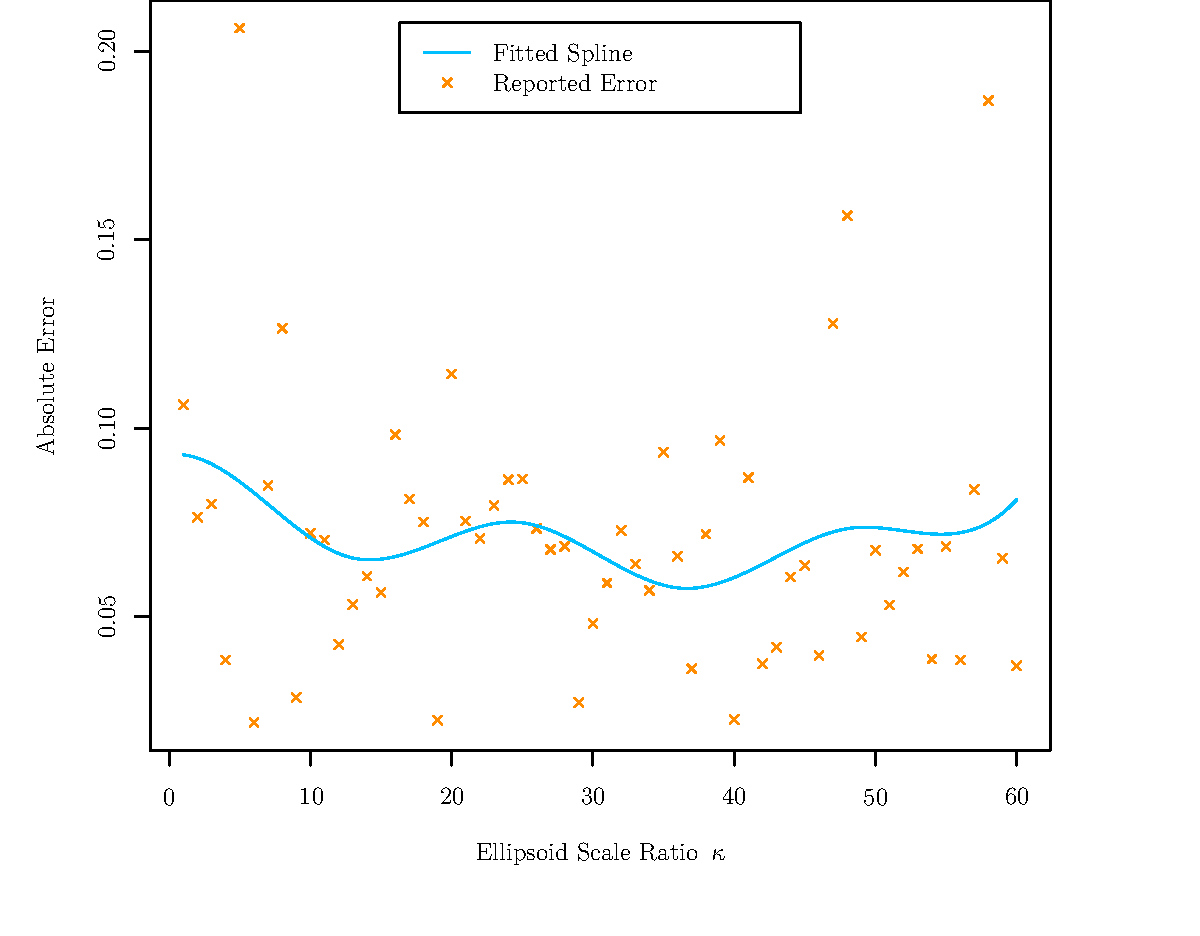
\includegraphics[width=140mm]{fig/fig_CSN.pdf}
  \else
  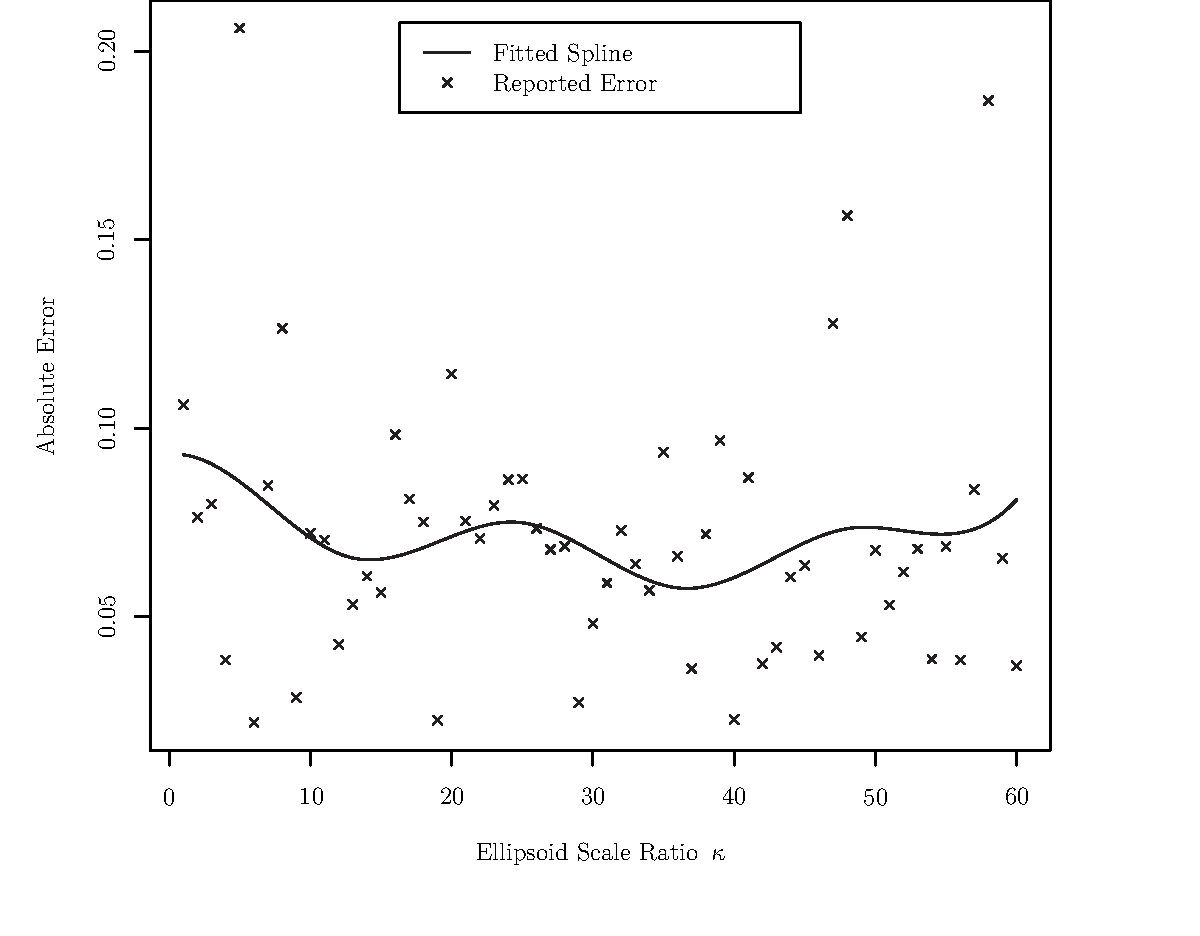
\includegraphics[width=140mm]{fig/fig_CSN_bw.pdf}
  \fi
  \makeatother
\end{figure}
\paragraph{隐私主成分分析输出维度$k$} % (fold)
\label{par:隐私主成分分析输出维度_k_}
输出维度$k$对算法精确性的影响是微妙的, 一方面, 增大$k$可以更好地概括原始数据集的分布信息, 但另一方面, 由算法\ref{alg:保证epsilon,delta差分隐私的子空间迭代算法}, $k$增大每一步增加的噪音也会相应增大, 从图\ref{fig:CRM数据集最坏绝对误差与隐私主成分分析输出维数_k}来看, $k$的增加对误差的影响方向并不确定. 
% paragraph 隐私主成分分析输出维度_k_ (end)
\begin{figure}[hbtp]\centering
  \caption{CRM数据集最坏绝对误差与隐私主成分分析输出维数$k$, 隐私设定为$(\epsilon, \delta)$-差分隐私, 其中$C=10^4, R = 102, L = 10, \kappa = 7$, 每次实验重复10次取平均值 }\label{fig:CRM数据集最坏绝对误差与隐私主成分分析输出维数_k}
  % \vskip\baselineskip % This is a dirty hack so just remove it if the figure is OK.
  \makeatletter
  \ifpkuthssextra@opt@colorlinks
  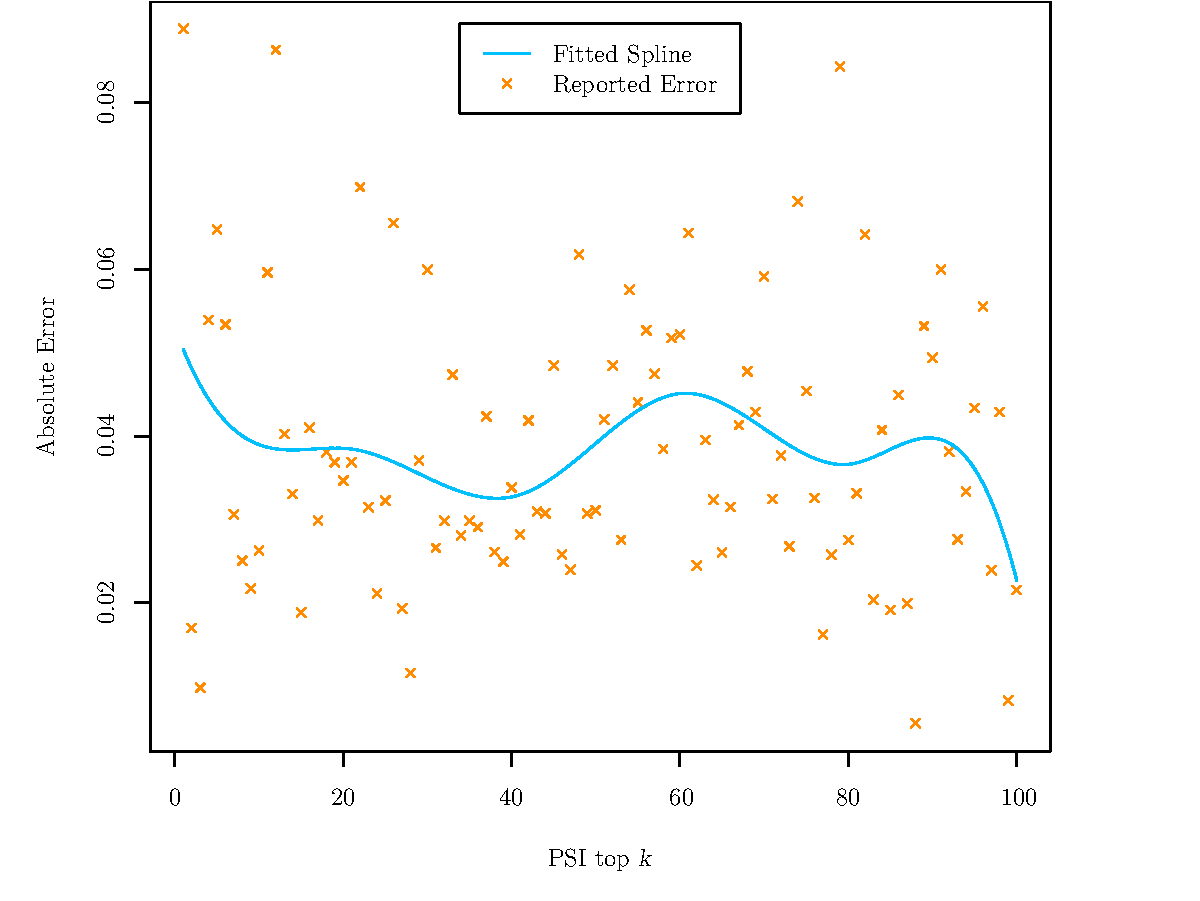
\includegraphics[width=140mm]{fig/fig_CRM.pdf}
  \else
  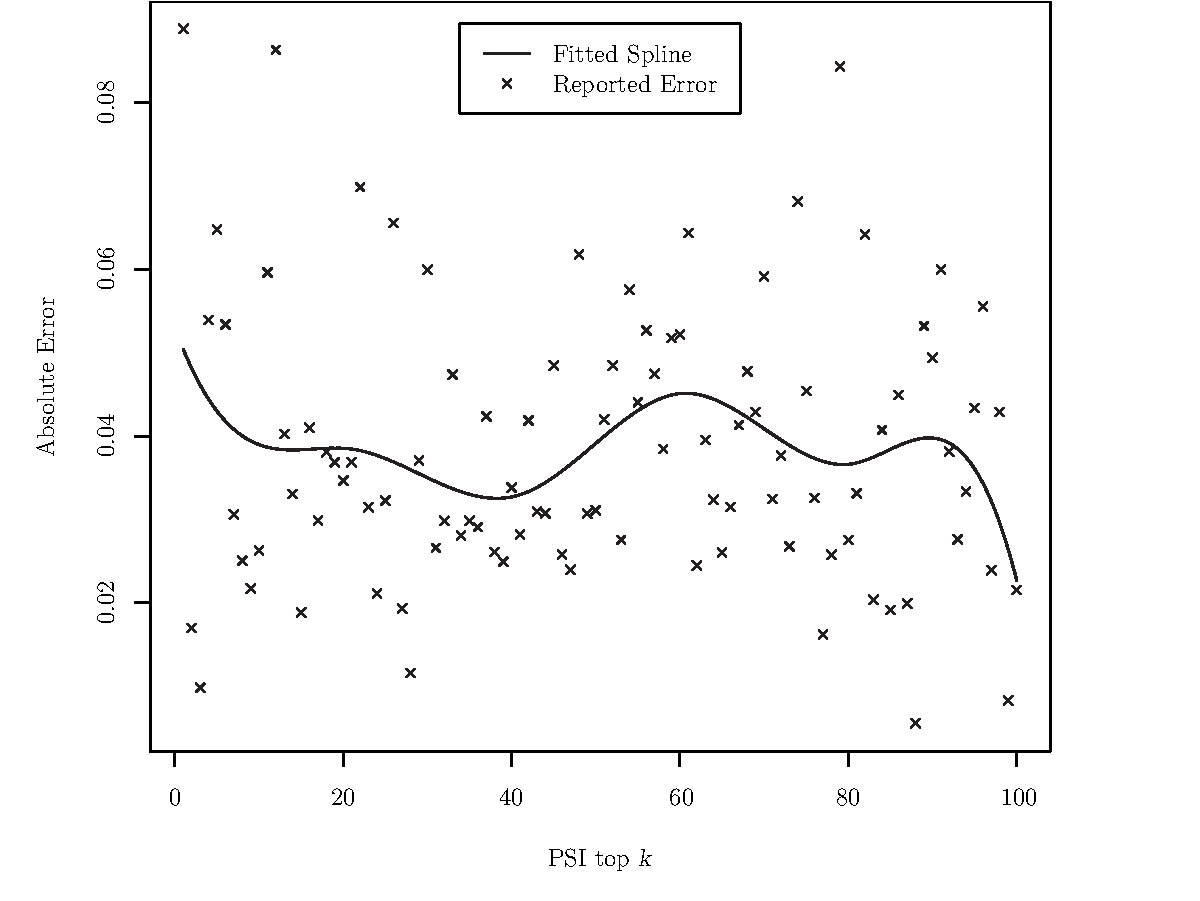
\includegraphics[width=140mm]{fig/fig_CRM_bw.pdf}
  \fi
  \makeatother
\end{figure}
% section 误差与部分参数关系 (end)
% chapter 实验 (end)
	% 结论。
	\specialchap{结论}
三角机制作为一个输出合成数据库的隐私机制无疑有着广泛的应用前景. 该合成数据库一方面保证了原始数据库的隐私, 另一方面对一大类统计查询 ------ 光滑查询提供了精确度保证. 更重要的是, 三角机制的时间代价关于原始数据的观测数的多项式, 而对目前已有的适用该问题的隐私机制, 其时间代价是超指数的. 对于高度光滑的查询, 三角机制保证了$O(n^{-1})$的精确度, 远远优于抽样误差$O\left(n^{-1/2}\right)$. 三角机制的实际运行时间还可以通过查询基与格点抽样来得到显著改善, 并通过隐私主成分分析来弥补部分损失的精确度. 在选定数据库上的实验结果支持三角机制的理论结果.

三角机制针对光滑查询可以给出精确的回答, 但现实中许多查询是非光滑的, 甚至是不连续的: 比如最常见的计数查询, 再如\parencite{blum2013learning}研究的矩形查询. 我们希望设计一种通用的隐私机制: 该机制可以回答除了光滑查询外, 还可以回答部分重要的离散查询的通用隐私机制, 该机制需要输出合成数据库, 还要尽可能高效. 如前所述, 对于简单的两参数查询, 输出合成数据库的隐私机制是指数时间的\parencite{ullman2011pcps}, 因此, 这个问题是非平凡的. 

最后, 三角机制要求数据库的域为$[-1, 1]^d$, 因而三角机制只能处理连续型的变量, 而对于离散型的多值分类变量, 是否可以用三角机制进行类似处理并保证一定的精度? 三角机制输出的合成数据库是连续的, 合成数据库应该如何进行离散化处理来保证离散型的变量体现在合成数据库中仍旧保持离散, 同时保证精度? 这些问题都是值得研究的方向. 

	% 正文中的附录部分。
	% \appendix
  % \titleformat{\chapter}[hang]
  % {\vspace{40pt}\heiti\bfseries\zihao{1}\centering}
  % {}
  % {1em}{}
	% 排版参考文献列表。
  \printbibliography[
    % 使“参考文献”出现在目录中;\textsc{如果同时要使参考文献列表参与章节编号},
    % 可将“bibintoc”改为“bibnumbered”。
    % heading = bibintoc,
    heading = bibintocWithStyle,
    nottype = misc
    % 单独设定排序方案。此设定会局部覆盖之前的全局设置。
    % 注:只有同时使用 2.x 或之后版本的 biblatex 和相应兼容版本的 biber,
    % 才能对每个 \printbibliography 命令采用不同的排序方案,
    % 否则只能在导入 biblatex 宏包时就(全局)指定排序方案。
    % 在这样的情况下,请去掉所有的 sorting 选项,否则可能出错。
    % sorting = ecnty
  ]
  \printbibliography[
    title = {数据集},
    heading = bibintocWithStyle,
    type = misc
  ]
	% 各附录。
	% % vim:ts=4:sw=4
% Copyright (c) 2014 Casper Ti. Vector
% Public domain.

\chapter{附件}




	% 以下为正文之后的部分。
	\backmatter

	% 原创性声明和使用授权说明。
	% vim:ts=4:sw=4
%
% Copyright (c) 2008-2009 solvethis
% Copyright (c) 2010-2013 Casper Ti. Vector
% All rights reserved.
%
% Redistribution and use in source and binary forms, with or without
% modification, are permitted provided that the following conditions are
% met:
%
% * Redistributions of source code must retain the above copyright notice,
%   this list of conditions and the following disclaimer.
% * Redistributions in binary form must reproduce the above copyright
%   notice, this list of conditions and the following disclaimer in the
%   documentation and/or other materials provided with the distribution.
% * Neither the name of Peking University nor the names of its contributors
%   may be used to endorse or promote products derived from this software
%   without specific prior written permission.
% 
% THIS SOFTWARE IS PROVIDED BY THE COPYRIGHT HOLDERS AND CONTRIBUTORS "AS
% IS" AND ANY EXPRESS OR IMPLIED WARRANTIES, INCLUDING, BUT NOT LIMITED TO,
% THE IMPLIED WARRANTIES OF MERCHANTABILITY AND FITNESS FOR A PARTICULAR
% PURPOSE ARE DISCLAIMED. IN NO EVENT SHALL THE COPYRIGHT HOLDER OR
% CONTRIBUTORS BE LIABLE FOR ANY DIRECT, INDIRECT, INCIDENTAL, SPECIAL,
% EXEMPLARY, OR CONSEQUENTIAL DAMAGES (INCLUDING, BUT NOT LIMITED TO,
% PROCUREMENT OF SUBSTITUTE GOODS OR SERVICES; LOSS OF USE, DATA, OR
% PROFITS; OR BUSINESS INTERRUPTION) HOWEVER CAUSED AND ON ANY THEORY OF
% LIABILITY, WHETHER IN CONTRACT, STRICT LIABILITY, OR TORT (INCLUDING
% NEGLIGENCE OR OTHERWISE) ARISING IN ANY WAY OUT OF THE USE OF THIS
% SOFTWARE, EVEN IF ADVISED OF THE POSSIBILITY OF SUCH DAMAGE.

% 原创性声明和使用授权说明页不需要装订到论文中,故不显示页码。
\cleardoublepage\thispagestyle{empty}
\newgeometry{height = 240mm, width = 150mm, ignoreheadfoot, vcentering}
{
	\vspace*{\fill}\linespread{1.5}\selectfont
	\centerline{\heiti\bfseries\Large 北京大学学位论文原创性声明和使用授权说明}

	\vskip 4em
	\centerline{\heiti\bfseries\Large 原创性声明}
	\vskip 1em

	本人郑重声明:
	所呈交的学位论文,是本人在导师的指导下,独立进行研究工作所取得的成果。
	除文中已经注明引用的内容外,
	本论文不含任何其他个人或集体已经发表或撰写过的作品或成果。
	对本文的研究做出重要贡献的个人和集体,均已在文中以明确方式标明。
	本声明的法律结果由本人承担。
	\vskip 1em
	\rightline
	{%
		论文作者签名:\hspace{5em}%
		日期:\hspace{2em}年\hspace{2em}月\hspace{2em}日%
	}

	\vskip 4em
	\centerline{\heiti\bfseries\Large 学位论文使用授权说明}
	\centerline{\zihao{-4}(必须装订在提交学校图书馆的印刷本)}
	\vskip 1em

	本人完全了解北京大学关于收集、保存、使用学位论文的规定,即:
	\begin{itemize}
		\item 按照学校要求提交学位论文的印刷本和电子版本;
		\item 学校有权保存学位论文的印刷本和电子版,
			并提供目录检索与阅览服务,在校园网上提供服务;
		\item 学校可以采用影印、缩印、数字化或其它复制手段保存论文;
		\item 因某种特殊原因需要延迟发布学位论文电子版,
			授权学校在 $\square$\nobreakspace{}一年 / %
			$\square$\nobreakspace{}两年 / %
			$\square$\nobreakspace{}三年以后在校园网上全文发布。
	\end{itemize}
	\par(保密论文在解密后遵守此规定)
	\vskip 1em
	\rightline
	{%
		论文作者签名:\hspace{5em}导师签名:\hspace{5em}%
		日期:\hspace{2em}年\hspace{2em}月\hspace{2em}日%
	}

	% 若需排版二维码,请将二维码图片重命名为“barcode”,
	% 转为合适的图片格式,并放在 img/ 目录中,然后去掉下面 2 行的注释。
	\vskip 4em \noindent
  
\includegraphics[height = 3em]{img/barcode}

	\vspace*{\fill}\par
}
\restoregeometry


\end{document}